\documentclass[12pt, a4paper, twoside]{report}
%%% Nyomtatásnál Figyelni a kétoldalasságra és a kötésre!!!
\usepackage{verbatim}
\usepackage[T1]{fontenc}
\usepackage[utf8]{inputenc}
%\usepackage[UTF8]{ctex}     %% kínai karakterekhez
\usepackage{anysize}
\usepackage[left=4cm,top=3cm, bottom=3cm, right=3cm]{geometry}
%\usepackage{cite}
%\usepackage[square,numbers]{natbib}
%\bibliographystyle{abbrvnat}



%\usepackage{xcolor}
\usepackage[table,xcdraw]{xcolor}
\colorlet{RED}{red}
\usepackage{amsmath}
\usepackage{mathtools}
\newcommand{\norm}[1]{\left\lVert#1\right\rVert}
\usepackage{amssymb}
\usepackage{eurosym}
\usepackage{graphics}
\usepackage{graphicx} %===!!!=== Ezt én adtam hozzá
\usepackage{caption} %===!!!=== Ezt én adtam hozzá
\usepackage{subcaption} %===!!!=== Ezt én adtam hozzá
%\usepackage{subfig}
%\usepackage{subfigure}
\usepackage{tikz}
\usepackage{pgfplots}
\pgfplotsset{compat=1.9}
\usepackage{pgfpages}
\usepackage{soul}
\usepackage{algorithm}
\usepackage{algpseudocode}
\makeatletter
\def\BState{\State\hskip-\ALG@thistlm}
\makeatother

\usepackage{color}
\usepackage{gensymb}
\usepackage{setspace}
\usepackage{circuitikz}
\usepackage{indentfirst}
\usepackage{pgfplotstable}
\usepackage{siunitx}
%\usepackage{subfigure}
\usepackage{fancyhdr}
\usepackage{multirow}
\pagestyle{fancy}
\fancyhead{}
\fancyhead[RO]{\textsl{\rightmark}}
\fancyhead[LE]{\textsl{\leftmark}}
%\usetikzlibrary{external}
%\tikzexternalize % activate!
\usepackage{breqn}
\usepackage[absolute,overlay]{textpos}
\usepackage{transparent}
\usepackage{eso-pic}
\usetikzlibrary{calc}
\usepackage{lscape}
\usetikzlibrary{circuits.logic.US,circuits.logic.IEC}
\usepackage{multirow}
\usepackage{hhline}
\usepackage{textpos}

%% Saját package-ek
\usepackage{textcomp}
\usepackage{mfirstuc}
\usepackage{longtable}
\usepackage{textcomp}
\usepackage{tabu}
\usepackage[shortlabels]{enumitem}
\usepackage{arydshln}
\setlength{\dashlinedash}{0.2pt}
\setlength{\dashlinegap}{4.5pt}
\setlength{\arrayrulewidth}{0.2pt}
\usepackage{tabularx}
\usepackage{ltablex}\keepXColumns
\usepackage{adjustbox}
%\usepackage{hyperref}
\usepackage{enumitem}
\newlist{inparaenum}{enumerate}{2}% allow two levels of nesting in an enumerate-like environment
\setlist[inparaenum]{nosep}% compact spacing for all nesting levels
\setlist[inparaenum,1]{label=\bfseries\roman*.}% labels for top level
\setlist[inparaenum,2]{label=\roman{inparaenumi}\emph{\alph*})}% labels for second level

\usepackage[backend=bibtex, style=ieee, sorting=none, defernumbers=true, url=false, doi=false]{biblatex} %%% true/fals be és kikapcsolás!!
\addbibresource{dolgozat} %bib fájl
% use boldface for specific author in biblatex bibliography
% http://tex.stackexchange.com/questions/73136/make-specific-author-bold-using-biblatex
%
% usage:
% % use boldface for specific author in biblatex bibliography
% http://tex.stackexchange.com/questions/73136/make-specific-author-bold-using-biblatex
%
% usage:
% % use boldface for specific author in biblatex bibliography
% http://tex.stackexchange.com/questions/73136/make-specific-author-bold-using-biblatex
%
% usage:
% \input{boldauthorname}
% ...
% \begin{document}
% \boldname{Doe}{John}{J.}
% \printbibliography
% \end{document}
%
% deactivate:
% \boldname{}{}{}
%
\def\makenamesetup{%
  \def\bibnamedelima{~}%
  \def\bibnamedelimb{ }%
  \def\bibnamedelimc{ }%
  \def\bibnamedelimd{ }%
  \def\bibnamedelimi{ }%
  \def\bibinitperiod{.}%
  \def\bibinitdelim{~}%
  \def\bibinithyphendelim{.-}}
\newcommand*{\makename}[2]{\begingroup\makenamesetup\xdef#1{#2}\endgroup}

\newcommand*{\boldname}[3]{%
  \def\lastname{#1}%
  \def\firstname{#2}%
  \def\firstinit{#3}}
\boldname{}{}{} %% több keresztnév esetén nem space kell hanem ~ karakter !!!!

% Patch new definitions
%%%%%%%%%%%%%%%%%% saját módosított változat %%%%%%%%%%%%%%%%%%%%%%
\renewcommand{\mkbibnamegiven}[1]{%
  \makename{\currfname}{#1}%
  \makename{\findfname}{\firstname}%
  \makename{\findinit}{\firstinit}%
  \ifboolexpr{ test {\ifdefequal{\currfname}{\findfname}} or test {\ifdefequal{\currfname}{\findinit}} }%
    {\kern-0.4em}
    {\kern-0.4em}%
}

\renewcommand{\mkbibnamefamily}[1]{%
  \makename{\currlname}{#1}%
  \makename{\findlname}{\lastname}%
  \ifboolexpr{ test {\ifdefequal{\currlname}{\findlname}} }%
    {\ifboolexpr{ test {\ifdefequal{\currfname}{\findfname}} or test {\ifdefequal{\currfname}{\findinit}} }
        {\mkbibbold{\currfname~\currlname}}
        {\currfname~\currlname}
    }
    {\currfname~\currlname}%
} 

%%%%%%%%%%%%%%%%%%%%%% eredeti ez volt %%%%%%%%%%%%%%%%%%%%
%\renewcommand{\mkbibnamegiven}[1]{%
%  \makename{\currname}{#1}%
%  \makename{\findname}{\firstname}%
%  \makename{\findinit}{\firstinit}%
%  \ifboolexpr{ test {\ifdefequal{\currname}{\findname}}%
%    or test {\ifdefequal{\currname}{\findinit}} }%
%  {\mkbibbold{#1}}{#1}%
%}
%
%\renewcommand{\mkbibnamefamily}[1]{%
%  \makename{\currname}{#1}%
%  \makename{\findname}{\lastname}%
%  \ifboolexpr{ test {\ifdefequal{\currname}{\findname}} }%
%  {\mkbibbold{#1}}{#1}%
%}


% ...
% \begin{document}
% \boldname{Doe}{John}{J.}
% \printbibliography
% \end{document}
%
% deactivate:
% \boldname{}{}{}
%
\def\makenamesetup{%
  \def\bibnamedelima{~}%
  \def\bibnamedelimb{ }%
  \def\bibnamedelimc{ }%
  \def\bibnamedelimd{ }%
  \def\bibnamedelimi{ }%
  \def\bibinitperiod{.}%
  \def\bibinitdelim{~}%
  \def\bibinithyphendelim{.-}}
\newcommand*{\makename}[2]{\begingroup\makenamesetup\xdef#1{#2}\endgroup}

\newcommand*{\boldname}[3]{%
  \def\lastname{#1}%
  \def\firstname{#2}%
  \def\firstinit{#3}}
\boldname{}{}{} %% több keresztnév esetén nem space kell hanem ~ karakter !!!!

% Patch new definitions
%%%%%%%%%%%%%%%%%% saját módosított változat %%%%%%%%%%%%%%%%%%%%%%
\renewcommand{\mkbibnamegiven}[1]{%
  \makename{\currfname}{#1}%
  \makename{\findfname}{\firstname}%
  \makename{\findinit}{\firstinit}%
  \ifboolexpr{ test {\ifdefequal{\currfname}{\findfname}} or test {\ifdefequal{\currfname}{\findinit}} }%
    {\kern-0.4em}
    {\kern-0.4em}%
}

\renewcommand{\mkbibnamefamily}[1]{%
  \makename{\currlname}{#1}%
  \makename{\findlname}{\lastname}%
  \ifboolexpr{ test {\ifdefequal{\currlname}{\findlname}} }%
    {\ifboolexpr{ test {\ifdefequal{\currfname}{\findfname}} or test {\ifdefequal{\currfname}{\findinit}} }
        {\mkbibbold{\currfname~\currlname}}
        {\currfname~\currlname}
    }
    {\currfname~\currlname}%
} 

%%%%%%%%%%%%%%%%%%%%%% eredeti ez volt %%%%%%%%%%%%%%%%%%%%
%\renewcommand{\mkbibnamegiven}[1]{%
%  \makename{\currname}{#1}%
%  \makename{\findname}{\firstname}%
%  \makename{\findinit}{\firstinit}%
%  \ifboolexpr{ test {\ifdefequal{\currname}{\findname}}%
%    or test {\ifdefequal{\currname}{\findinit}} }%
%  {\mkbibbold{#1}}{#1}%
%}
%
%\renewcommand{\mkbibnamefamily}[1]{%
%  \makename{\currname}{#1}%
%  \makename{\findname}{\lastname}%
%  \ifboolexpr{ test {\ifdefequal{\currname}{\findname}} }%
%  {\mkbibbold{#1}}{#1}%
%}


% ...
% \begin{document}
% \boldname{Doe}{John}{J.}
% \printbibliography
% \end{document}
%
% deactivate:
% \boldname{}{}{}
%
\def\makenamesetup{%
  \def\bibnamedelima{~}%
  \def\bibnamedelimb{ }%
  \def\bibnamedelimc{ }%
  \def\bibnamedelimd{ }%
  \def\bibnamedelimi{ }%
  \def\bibinitperiod{.}%
  \def\bibinitdelim{~}%
  \def\bibinithyphendelim{.-}}
\newcommand*{\makename}[2]{\begingroup\makenamesetup\xdef#1{#2}\endgroup}

\newcommand*{\boldname}[3]{%
  \def\lastname{#1}%
  \def\firstname{#2}%
  \def\firstinit{#3}}
\boldname{}{}{} %% több keresztnév esetén nem space kell hanem ~ karakter !!!!

% Patch new definitions
%%%%%%%%%%%%%%%%%% saját módosított változat %%%%%%%%%%%%%%%%%%%%%%
\renewcommand{\mkbibnamegiven}[1]{%
  \makename{\currfname}{#1}%
  \makename{\findfname}{\firstname}%
  \makename{\findinit}{\firstinit}%
  \ifboolexpr{ test {\ifdefequal{\currfname}{\findfname}} or test {\ifdefequal{\currfname}{\findinit}} }%
    {\kern-0.4em}
    {\kern-0.4em}%
}

\renewcommand{\mkbibnamefamily}[1]{%
  \makename{\currlname}{#1}%
  \makename{\findlname}{\lastname}%
  \ifboolexpr{ test {\ifdefequal{\currlname}{\findlname}} }%
    {\ifboolexpr{ test {\ifdefequal{\currfname}{\findfname}} or test {\ifdefequal{\currfname}{\findinit}} }
        {\mkbibbold{\currfname~\currlname}}
        {\currfname~\currlname}
    }
    {\currfname~\currlname}%
} 

%%%%%%%%%%%%%%%%%%%%%% eredeti ez volt %%%%%%%%%%%%%%%%%%%%
%\renewcommand{\mkbibnamegiven}[1]{%
%  \makename{\currname}{#1}%
%  \makename{\findname}{\firstname}%
%  \makename{\findinit}{\firstinit}%
%  \ifboolexpr{ test {\ifdefequal{\currname}{\findname}}%
%    or test {\ifdefequal{\currname}{\findinit}} }%
%  {\mkbibbold{#1}}{#1}%
%}
%
%\renewcommand{\mkbibnamefamily}[1]{%
%  \makename{\currname}{#1}%
%  \makename{\findname}{\lastname}%
%  \ifboolexpr{ test {\ifdefequal{\currname}{\findname}} }%
%  {\mkbibbold{#1}}{#1}%
%}


\usepackage{sectsty}

%\usepackage{ulem}
%\newcommand{\soutthick}[1]{%
%    \renewcommand{\ULthickness}{2.4pt}%
%       \sout{#1}%
%    \renewcommand{\ULthickness}{.4pt}% Resetting to ulem default
% \usepackage{MnSymbol,wasysym}
%\DeclareSourcemap{
  %\maps[datatype=bibtex]{
    %\map{
      %\step[fieldsource=issue, match=\regexp{\A(\d+)\Z}, final]
      %\step[fieldset=number, fieldvalue={$1}]
      %\step[fieldset=issue, null]
    %}
  %}
%}

\newcommand{\myparagraph}[1]{\paragraph{#1}\mbox{}\\}


\def\myuni{Universiy of Pannonia}
\def\myfaculty{Department of Electrical Engineering and Information Systems}
\def\myschool{Doctoral School of Information Science}
\def\mytitle{Optimal Current Control for Domestic Power converters}
\def\myauthor{L\'aszl\'o Rich\'ard Neukirchner}
\def\mydate{2020}
\def\mysupervisor{dr. Attila Magyar}


%\rhead{L\'aszlo Richard Neukirchner (ZOK4EW) 2014/15/II.}
\renewcommand{\contentsname}{List of contents}
\renewcommand{\figurename}{Figure}
\renewcommand{\tablename}{Table}
\renewcommand{\chaptername}{Chapter}
\renewcommand{\bibname}{Bibliography}
\let\oldref\ref
\renewcommand{\ref}[1]{(\oldref{#1})}
%\newcommand{\norm}[1]{\left\lVert#1\right\rVert}

\newcommand{\sig}[1]{\begin{tikzpicture} \draw[ultra thick, densely dotted, color=white] (0,0)--(8,0) ;\draw[ultra thick, dotted] (10,0)--(14,0) (12,0) node[below]{#1};  \end{tikzpicture}}


\setcounter{secnumdepth}{2}
%% esetleges jelölések definiálása a későbbi változtatások gyors bevezetésére a dokumentumban
\newcommand{\Temp}[2]{T_{#1}^{#2}}        % hőmérsékletek 
\newcommand{\HeatTr}[2]{K_{#1}^{#2}}      % hőveszteség
\newcommand{\HeatCap}[2]{C_{#1}^{#2}}      % hőkapacitás
          %%


\begin{document}

 \pagenumbering{Roman}

        %% első üres oldal
 \null
 \thispagestyle{empty}%
 \addtocounter{page}{-1}%
 \newpage

%% Title Page
 \thispagestyle{empty}%
\begin{center}
    \myuni \\
    \myfaculty \\
    \myschool \\[0.6cm]
    
\includegraphics[width=4cm]{img/MIK_cimer.jpg}\\[1.2cm]
    \begin{spacing}{2} \fontsize{25}{15}\textbf{ \textsc{\mytitle} }\end{spacing} %\\[1cm]
    DOI:.................... \\[1.5cm]
    Doctoral (PhD) Thesis \\
    Author: \myauthor \\[1cm]
    Supervisor: \mysupervisor \\[1.5cm]
    Made at \myuni \myschool  \\[1.5cm]
    Veszpr\'em \\
    \mydate
\end{center}

\newpage 

%% Mandatory third page
 \thispagestyle{plain}
\begin{center}
    {\fontsize{14}{8}\textbf{\textsc{\mytitle}}} \\[1cm]
    Értekezés doktori (PhD) fokozat elnyerése érdekében\\[0.3cm]
    Írta:\\
    {\textbf \myauthor}\\[0.3cm]
    Készült a \myuni \myschool keretében \\[0.3cm]
\end{center}
Témavezető: \mysupervisor \\
Elfogadásra javaslom: igen / nem\\
\sig{aláírás}\\[0.7cm]
A jelölt a doktori szigorlaton ........... \%-ot ért el. \\[1cm]
Az értekezést bírálóként elfogadásra javaslom: \\[0.3cm]
Bíráló neve: ........................................ : igen / nem\\
\sig{aláírás}\\[0.7cm]
Bíráló neve: ........................................ : igen / nem\\
\sig{aláírás}\\[0.7cm]
A jelölt az értekezés nyilvános vitáján ........... \%-ot ért el.\\
Veszprém, ...................\\[0.5cm]
\sig{a Bíráló Bizottság elnöke}\\[1cm]
A doktori (PhD) oklevél minősítése: ..................................\\[1cm]
\sig{az  EDHT elnöke}\\



\newpage 

%% Acknowledgements
 \chapter*{Acknowledgement}
\thispagestyle{plain}
I wish everybody the best! 



%\chapter*{Compendiary} --> Not required
% \input{subtex/0000_compendiary.tex}
%% (max 2500 karakter)

%% Abstract
\chapter*{Abstract}
\thispagestyle{plain}
Tryout \cite{thrift2003space}!
     Voltage unbalance is a major yet often overlooked power quality problem in low voltage residential feeders due to the random location and rating of single-phase renewable sources and uneven distribution of household loads. This paper proposes a new indicator of voltage \textcolor{red}{deviation} that may serve as a basis of analysis and compensation methods in this dimension of power quality. The paper proposes three main results. First of all a novel voltage norm capable of indicating unbalance and \textcolor{red}{under-voltage in a single value. Afterwards,} a three phase unbalance reduction controller structure is given. As the third main result, the proposed controller structure is integrated with an optimization based control algorithm that uses asynchronous parallel pattern search as its engine. The suggested structure and the underlying three phase power grid model has been implemented in a dynamical simulation environment and tested against engineering expectations.
    The simulation based experiments served as a proof of concept for the proposed complex control structure. The experiments included performance and robustness analysis, both of them concluded that the proposed control and inverter structure is promising.
    The proposed three phase inverter structure together with the control algorithm connected with a renewable source (photovoltaic panel or wind turbine) is capable of an asymmetric power injection \textcolor{magenta}{or rerouting the energy flow} to the grid so that the voltage unbalance decrease. This is also important from the environmental point of view since the achieved power loss reduction can easily be translated to $\textnormal{CO}_2$ emission reduction and carbon footprint - these indicators has also been calculated.===\\ 
    This Thesis is consisted about optimal control of power converters. The firs part is consisting of a constrained optimal control of a current source rectifier (CSR) is presented, based on a mathematical model developed in Park's frame. To comply with the system constraints an explicit model-based predictive controller was established. To simplify the control design, a disjointed model was utilised due to the significant time constant differences between the AC and DC side dynamics. As a result, active damping was used on the AC side, and explicit Model Predictive Control (MPC) on the DC side. The results are compared by simulation with the performance of a state feedback control. This is followed by developing a cost function for mitigating voltage asymmetry on a domestic network, which requires only measuring the voltage whist only current interventions are required. Lastly an asymmetric inverter structure was developed to serve the const function minimizing compensational needs. Results were implemented and validated with Matlab simulations.

%\newpage
%
%\thispagestyle{plain}
%\chapter*{ (3. nyelven) \normalfont{抽象}}
%(max 8-10 sor)




%% Tableofcontents
\thispagestyle{plain}
\tableofcontents
\newpage

\pagenumbering{arabic}

%% Introduction
\chapter{Introduction}

%==== Free text =====================================================
Growth of distributed generation from renewable energy sources and the nature of the electrical power grid initiated a trend to alter from a passive network to an active one. So called smart grids have the ability to provide much more in depth observable measurement results of they customers, gird operators and energy traders alike. Through voltage and current measurements, the habits of each actor (household, station, or industrial- commercial facility) can be easily mapped and taken into account. Moreover, the potential failure could be indicated and preemptively acted upon, before irreversible malfunction, significant amount of wear, or generally, the efficiency of energy consuming actor's power electric consumer's diminishes. In most cases, only smart metering is present, whilst central control and measurement is not an option.\\
 In this new environment, the importance and difficulty of maintaining and operational stability and cost effective control of the distribution system are increasing together. With this in mind local solutions are the most convenient solutions, and as opposed to this expectation most of a household's possible renewable sources and loads are unevenly distributed, without mindful control over single phase power converters. Some of these could represent an unevenly high power consumption, or worse a locally significant energy source in times where it's most unnecessary, especially outside peak zones of consumption. The situation is further exacerbated by the stochastic on/off switching of the different types of loads which causes stochastic disturbing unbalance in the load currents which cases unbalanced load of the low voltage transformer, and causes amplitude and phase unbalance in the voltage phasor trough the serial impedance of the low voltage transportation line wires and connecting devices cables.\\
If we observe the opposite side, ideal generators supply symmetrical three-phase sinusoidal (mostly only) positive sequence voltages, which are balanced in terms of their amplitudes phase differences at a single frequency. With this in mind, without taking the said gap, voltage (as such consumption- and production-) unbalance occurs on the network. The terminology of unbalance can be divided into amplitude unbalance, phase difference unbalance, and unbalanced harmonic disturbance. The occurrence of at least one of these features is enough for a distribution network to become unbalanced. \\
Many countries have changed their regulating laws about power supply to allow for grid-tie inverter systems to provide spare power from renewable sources to local low voltage grids.The unbalance of the grid is further increased by using single phase grid tie inverter systems in the size of typical small household power plants (1 - 50\,kW) and the produced electrical power originating from renewable power source (wind and solar) also admits stochastic behavior. This unbalance yields to a suboptimal operation of low voltage three phase transformers and machines to generate undesirable additional yield loss and increase in the probability of malfunction of the low voltage energy transportation system's components, or the effective current unbalance could cause additional power loss of the transportation line resistances or in the end complete shutdown.\\
To mitigate or avoid such situations an approach is required, where the system where said phenomena occurs is an optimization problem. However to formulate an optimization problem, many things should be layd down to formulate it properly. Most importantly, a cost function should be established which can bi served as a local (or global minima) for solving the question. For instance, if voltage unbalance would be eliminated, than the correct indicator of unbalance should serve as basis, moreover the deviation from the optimum could be quadratic.\\
Such tasks can not be achieved without proper instrumentation. To be able to apply control, where he voltage levels are designated, and the end user has no direct control (only the plant or transformer level has such), deviations can be addressed, and current control can be used as actuation. This way a control structure can be imagined for a power electric converter, where every step should cont towards the optimum state, with respect of the energy (or control reserves), wear of the device (sub components, namely gates have finite switching capabilities), and  safety constraints ( designated level of current and voltage should not trespass a given hard constraint for the sake of malfunction avoidance, and soft constraint for the sake of reducing wear). Additionally it should not be forgotten, that with all the above, the device should operate in the domains of $kHz$ or above, and it shoud be run on a cheap device, like an embedded micro-controller chip or DSP. With all this in mind an the designed power electric structure can be designed to fulfill the high standers of today’s requirements. The problem is, conventional controllers can not achieve this all at once. The methodology based on optimal control, was originally designed for highly complex, and safety critical systems, with huge amount of inputs and outputs, power plants, and chemical- or refinery plants. This system though have an incomparably lower time constant, which renders conventional model based predictive controllers useless in the domain of power electronics. \\
To marry the two approaches together, a solution came up from the automotive industry. A car is also a highly safety critical multiple-input, multiple-output (MIMO) system with obvious constraints, in increasingly changing environment. The key is, to map said environment and in it every state, the system can, or allowed to achieve. Where contraints are present, finite states can be defined, eighter by hand (e.g. statemachies) or by advanced mapping algorythms, and then in every little kingdom, a relatively simple (linear if possible)  rule where one state of the system dynamics could be substituted, then to make sure stepping on to the next most applicable rule can be achieved very fast. This way, by choosing the resolution of the mapping correctly (too fine resolution gives too hich processing requirements, too low gives suboptimal dynamics), the predictive control approach can be applied in both worlds.\\
In this thesis..


\section{Literature overview}

%============ RENEWABLE SYSTEM
Single phase power injections to the grid are mainly generated by domestic photovoltaic-(PV) and wind power plants. Many current references about the renewable energy sources integration to the low voltage grid are short-, and long-time storage ready for connection of this electrical energy in the literature can be found. For off-grid, sometimes more complex solutions integrating diesel generators, PV and wind generators. Such as proposed, in \cite{shezan2016}. \cite{cucchiella2013environmental} where presented the economical aspects of a PV system. The economic results are strongly influenced by the annual average isolation value, which encourages the areas most exposed to the sun and the southern areas. The consumption of consumers is not critically important, but the design principle used has as significant effect on the maximization of the performance of PV plants. In \cite{kaldellis2009optimum} worth noticing, that autonomous photovoltaic systems are strongly responsible of their reactive energy requirements. To support photovoltaic systems with battery banks sustainable character one should be able to establish that their reactive energy requirement share fairly compensated by the corresponding energy yield.  Additionally, in \cite{ortega2013measurement} the author emphasizes that PV systems are increasingly being deployed in all over the world, and this is the source of a wide range of power quality problems. With a view to consistently measuring and assessing the power quality characteristics of PV systems, they had presented an in-depth overview and discussion of this topic.\\
%============ EV SYSTEM
 The study by \cite{huat2015integration} explored integration issues of electric vehicle battery packs. They suggest that high voltage battery packs with large format cells has advantages in assembly, thermal management, monitoring and control, services and maintenance. On the other hand, quality, reliability and limited specific energy of large format cells are obstacles need to overcome. Solving these problems will further affect the cost, performance, reliability and safety of the electric vehicles. Smart energy systems in specially in urban areas are discussed in \cite{lund2015smart} where a design methodology has been suggested.\\
%============ EFFECTS OF UNBALANCE
Many power systems, voltage parameters change over time. Variation of power quality disturbances leads to thermal transients in electrical machines. This problem can be especially important in the case of low-power machines, because they have shorter time constants than high-power ones. The rate of thermal responses of a machine also significantly depends on the type of power quality disturbances. Voltage unbalance can cause  machine  overheating  within  a  mere  few  minutes. Furthermore,  fluctuating  unbalance  could  cause  an  extraordinary rise  in  windings  temperature  and  additional  thermo-mechanical stress.  Consequently,  voltage  unbalance  is  found  to  be  more harmful to induction motors than the results from previous works \cite{gnacinski2019induction}. Additionally beside the heat factor, voltage unbalance can cause increased reactive power \cite{savaghebi2012secondary}, various copper loss \cite{siddique2004effects} torque pulsation in electric motors \cite{brekken2005control} have been studied. \cite{lee1998effects} were discussing the effects of unbalanced voltage on a three-phase induction motor, one has to consider not only negative-sequence voltage but also the positive-sequence voltage. With the same voltage unbalance factor, the status of voltage unbalance could be judged by the magnitude of positive sequence voltage. Also the effect of voltage unbalance has been studied on three-phase four-wire distribution networks for different control strategies for three-phase inverter-connected distributed generation units on voltage unbalance in distribution networks (\cite{meersman2011three}). Here the negative-sequence component and the zero sequence component were studied where unbalance conditions could lower stability margin and increasing the power losses. On the other hand, the adaptive coordination of distribution systems included distributed generation is also an emerging problem as it was discussed by \cite{ates2016}.  A small voltage unbalance might lead to a significant current unbalance because of low negative sequence impedance as highlighted in \cite{bina2011three}.\\
%============ DEPARTMENT WORK REGARDING UNBALANCE 
As such at the University of Pannonia a previous work of \cite{gorbe2012reduction} a complex control unit has been proposed that is capable of lowering extant harmonic distortion. In the work of \cite{Gorbe2014experimental} the effect of a small domestic (photovoltaic) power plant on the power quality, mainly the total harmonic distortion has been examined. The aim of this work is to examine and compensate three phase voltage asymmetry of the electrical network based on the extended simulation model proposed by \cite{gorbe2012reduction}. Further control methods were applied for the solution for balancing of the most sensitive with regard to electric energy quality part of power system in \cite{uimethod},  minimizing the active power losses, stabilization of three-phase voltages, enhancement of asynchronous machine performance stability and reduction of errors occurring in power consumption measuring circuits.\\
%============ UNBALANCE CALCULATION
In many articles the authors presents a different viewpoint of calculating unbalance on the network. \cite{martin2015unbalance} showed to assess the harmonic distortion and the unbalance introduced by the different loads connected to the same point of common coupling have been applied to an experimental distribution network.  By \cite{kini2007novel} the focus was to bring out the ambiguity that crops up when we refer to a particular value of voltage unbalance that exists in the system. By making use of the complex nature of voltage unbalance, the voltage combinations that lead to the calculation of complex voltage unbalance factor could be narrowed down to a great extent. A fast and accurate algorithm for calculating unbalance has been presented by \cite{wen2014approximate}. The magnitudes of zero, positive, and negative sequences are obtained through simple algebraic equations based on the geometric figure, which is also called as 4 and 8 geometric partitions. Also a three-phase optimal power flow calculation methodology has been presented by \cite{araujo2013three}, that is suitable for unbalanced power systems. The optimal algorithm uses the primal-dual interior point method as an optimization tool in association with the three-phase current injection method in rectangular coordinates.\\
%============ UNBALANCE COMPENSATION
There are different approaches of lowering the unbalance with different control techniques. Additionally, new computationally efficient control techniques have been presented by \cite{lee2009new} to estimate and compensate input voltage-unbalance disturbances for a voltage source converter. These tools are designed to be effective with high power systems with slower PWM switching frequencies of 5 kHz or lower and limited current-controller bandwidth. About the unbalance compensation control aspect, a three-phase IGBT-based static synchronous compensator were proposed for voltage and/or current unbalance compensation by \cite{xu2010voltage}. An instantaneous power theory was used for real-time calculation and control. Three control schemes current control, voltage control and integrated control were proposed to compensate unbalanced voltage, unbalanced current or both. Unbalance phenomena and power quality can be examined with modeling too. A particular modeling method was presented by \cite{li2005microgrid}, where a three-phase four-wire grid-interfacing power quality compensator were modeled. During grid voltage unbalance, the compensator, used a shunt and a series four phase inverter, and could enhance both the quality of power within the microgrid and the quality of currents flowing between the microgrid and utility system, where a microgrid is a group of interconnected loads and distributed energy resources within clearly defined electrical boundaries that acts as a single controllable entity with respect to the grid. A microgrid can connect and disconnect from the grid to enable it to operate in both grid-connected or island-mode. The shunt four-leg inverter were controlled to maintain a set of balanced distortion free voltages to regulate power sharing among the parallel-connected distributed generation systems. Simulation studies were carried out by \cite{Hu2016264} where one of the aims was to develop and test the feasibility of a decoupled three-phase on-load tap charger in the distribution system with the objective of improving the distribution network power quality. Further control methods were applied for the solution for balancing of the most sensitive with regard to electric energy quality part of power system by \cite{uimethod},  minimizing the active power losses, stabilization of three-phase voltages, enhancement of asynchronous machine performance stability and reduction of errors occurring in power consumption measuring circuits.\\
%============ UNBALANCE COMPENSATON WITH OF CURRENT SOURCE CONVERTERS
In the arsenal of voltage unbalance compensation, current source power electronic devices have a dedicated position. Based on the instantaneous active power theory under unbalanced  grid conditions \cite{wang2016dc} proposes an optimized negative-sequence current  references  for  eliminating  the double-frequency  oscillations  on  active  power  at  AC  side of a current source converter. The author argues in \cite{wang2014virtual} that a classification of the virtual impedances can greatly benefit an unbalance compensating control structure, with an active stabilization method. In \cite{guo2018advanced} direct control strategy with detailed current converter model is shown which is much simpler than the complicated instantaneous power theory approach. This solution needs less voltage and current sensors for the feedback control, which means that it is a cost-effective solution. An interesting, yet similar approach compared in the paper if a bi-directional current source topology is used like in \cite{vekhande2015control}. This enables to compensate a much larger degree of freedom handing unbalanced conditions with the precaution of unstable operation possibilities.\\
%============ USAGE OF CURRENT SOURCE RECTIFIERS
Current source rectifiers (CSR) are widely used in frond-end power electronic converter for the uncontrollable or controllable DC-bus in industrial and commercial applications. They have maintained their position through many applications, with uses such as medium-voltage high-power drives \cite{vajda2017limiting}, \cite{ghalem2010six} STATCOMs \cite{gupta2014two} and renewable systems \cite{chen2016single}, \cite{exposto2015predictive}. They have a plain and reliable circuit structure, which makes them attractive for simple control design. The CSRs are traditionally controlled by state feedback, or classic cascaded linear control loops such as PI controllers. These simple control applications are suitable for induction motor control \cite{chebre2011speed}, and other electromechanical actuators \cite{salloum2014robust}, and unusual topologies \cite{neukirchner2017voltage}. Also, worth mentioning of self-tuning variants of PI controllers \cite{tahri2012digital}.\\
%============ MODULATION OF CSR
 In the past, the modulation methods used were trapezoidal pulse width modulation techniques (TPWM), or application of pulse patterns calculated offline for selective harmonic elimination (SHE). More recently, current space vector modulation (SVM) has been used for the synthesis of the transistor control signals \cite{gao2017model}. Even so, AC-side harmonic elimination could still be an issue at lower switching frequencies where LCL filtering (inductive-capacitive-inductive) would be advised \cite{han2010control}.\\
%============ TOPOLOGIES OF CSR
In order to keep switching frequencies low and to minimize switching losses, new topologies and hybrid modulations are used, mixing TPWM and SHE depending on the grid frequency \cite{venkatraman2018multilevel}.\\
%============ BENEFITS OF CSR
    In terms of the amplitude of the grid and DC-link voltages, CSRs exhibit a step-down conversion. When used as DC voltage source, the rectifier can output a lower DC voltage without the need of a grid-side transformer, as is usually employed in voltage source rectifiers (VSR). Because of their current source behavior, CSRs can be easily paralleled and provide inherent short-circuit protection, representing an excellent potential in DC power supply applications \cite{feroura2017finite}, \cite{yan2015study}.\\		
%============ GENERAL POWER ELECTRIC CONTROL
    There are several control strategies in addition to classical PI control for applications in this domain. Self-adapting control methods are on the rise with more sophisticated algorithms in the field of fuzzy logic \cite{urmos2017application}. They are capable of handling increasingly more complicated models and systems with high dynamics and accuracy \cite{chatterjee2008augmented}, \cite{haidegger2012simulation}, and even without establishing and validating classical state-space models \cite{vrkalovic2018model}. The other filed is the sliding mode control, which can achieve good dynamic performance and handle non-linearity. Still, they might also introduce chattering, which can be very undesirable when applied to real-life systems like in \cite{regaya2014new} and \cite{szell2014mathematical}. Additionally in \cite{ahmed2014model} the validity of an MPC-based, digital pulse width modulation control strategy for single-phase voltage source rectifiers is discussed, further confirming the validity of this method in control systems.\\	
%============ PREDICTIVE POWER ELECTRIC CONTROL		
    In the linear domain implicit model predictive control (IMPC or just MPC) is a fair solution due its effectiveness in power electronics due to its configurable cost function and such scalable nature \cite{kelemen2010constrained}, \cite{ahmed2014model}. In this field also finite-state solutions are present which can be considered also predictive control, where the modulation scheme’s defined states serve as optimization potential \cite{rivera2013predictive}, \cite{godlewska2015predictive}. As a further step adaptive application was established to tackle parameter estimation problems for better performance \cite{muthukumar2016adaptive}\\	
%============ EXPLICIT PREDICTIVE CONTROL
    Recently, beside implicit, finite-state, and adaptive predictive control, explicit model predictive control has emerged in the field of power electronics \cite{kutasi2010constrained}. Establishing the MPC cost function can range widely depending on the expected dynamics, degree of noise cancellation, and model complexity. Additionally, the current limitation can also be implemented introducing constraints in the modulation algorithm.\\	

 %Not requied:
 %%% \section{Motiv\'aci\'o \'es c\'el}

\section{Motivation}

This stuff is so important and interesting! 
 %%\thispagestyle{plain}
%%\chapter*{Compendiary}
(max 2500 karakter)\\
Outline of the thesis.
%
%\newpage

%\thispagestyle{plain}
%%\chapter*{Abstarct}
% (max 8-10 sor)


%\newpage
%
%\thispagestyle{plain}
%\chapter*{ (3. nyelven) \normalfont{抽象}}
%(max 8-10 sor)





%% Basic notions
\chapter{Basic notions}\label{BASIC:sec:main}

In this chapter the basic topics of the thesis are discussed, as components for further understanding. First the phenomena of voltage unbalance on small distribution networks are shown and the ambiguities though the development of the concept, and at the end the norm currently being in use in the industry. It would be shown how many definitions are currently in use, thus the introduced ambiguity of definition, further validating the proposal in section \ref{VUB:sec:Geom}.\\
Next a necessary glimpse of power electric background is given to invite to the viewpoint of the modeling and problem breakdown of power converter. The section would introduce the background of current source switching devices with forced commutation, since control based on external situations or according to a cost function is eminent. After the single phase method shall be described, DC-DC conversion would be shown, since in section \ref{VUB:sec:Compensation} non-zero mean asymmetrical power injection was required. The section closes with the three phase rectifier example, for contributing the understating of the modeling in section \ref{EMPC:sec:Modeling}.\\
Lastly the basis of controller structures, shall be shown, applied in the thesis. These are the APPS (asynchronous parallel pattern search) method (used in section \ref{VUB:sec:Optimization}) and constrained model based predictive control (MPC) is to be described with the end with the explicit partition of the state space (explicit MPC applied in section \ref{EMPC:sec:DCside}) for a computationally efficient approach.

	\section{Definitions of voltage unbalance}\label{BASICUNB:sec:DefinitionsofUNB}

%\textbf{(Mostly) from Wikipedia:}\\
In a symmetric three-phase power supply system, three conductors each carry an alternating current of the same frequency and voltage amplitude relative to a common reference but with a phase difference of one third of a cycle between each. The common reference is usually connected to ground and often to a current-carrying conductor called the neutral. Due to the phase difference, the voltage on any conductor reaches its peak at one third of a cycle after one of the other conductors and one third of a cycle before the remaining conductor. This phase delay gives constant power transfer to a balanced linear load.\\
In general symmetric three-phase systems described, are simply referred to as three-phase systems because, although it is possible to design and implement asymmetric three-phase power systems (i.e., with unequal voltages or phase shifts), they are not used in practice because they lack the most important advantages of symmetric systems. In a three-phase system feeding a balanced and linear load, the sum of the instantaneous currents of the three conductors is zero. In other words, the current in each conductor is equal in magnitude to the sum of the currents in the other two, but with the opposite sign. The return path for the current in any phase conductor is the other two phase conductors.\\
Constant power transfer and cancelling phase currents would in theory be possible with any number (greater than one) of phases, maintaining the capacity-to-conductor material ratio that is twice that of single-phase power. However, two-phase power results in a less smooth (pulsating) torque in a generator or motor (making smooth power transfer a challenge), and more than three phases complicates infrastructure unnecessarily.\\
Three-phase systems may also have a fourth wire, particularly in low-voltage distribution. This is the neutral wire. The neutral allows three separate single-phase supplies to be provided at a constant voltage and is commonly used for supplying groups of domestic properties which are each single-phase loads. The connections are arranged so that, as far as possible in each group, equal power is drawn from each phase. Further up the distribution system, the currents are usually well balanced. Transformers may be wired in a way that they have a four-wire secondary but a three-wire primary while allowing unbalanced loads and the associated secondary-side neutral currents \cite{von2006electric}.

\subsection{Phenomena of voltage unbalance}\label{BASICUNB:sec:PhenomenafUNB}

In a domestic network, three-phase electric power systems have at least three conductors carrying alternating voltages that are offset in time by one-third of the period. A three-phase system may be arranged in delta  or star. A star system allows the use of two different voltages from all three phases, such as a 230/400 V system which provides 230 V between the neutral (center hub) and any one of the phases, and 400 V across any two phases displayed on Fig.\ref{BASICUNB:fig:UnbWave}. The definition is the following:
	
			\begin{equation}
        \begin{array}{rcl}
            \vec{V}_a&=&\hat{V}\,sin(\theta)\\
						\vec{V}_b&=&\hat{V}\,sin(\theta+\frac{4}{3}\pi)\\
						\vec{V}_c&=&\hat{V}\,sin(\theta+\frac{2}{3}\pi),\\
        \end{array}
        \label{BASICUNB:equ:Definition}
    \end{equation}
	
	where $\vec{V}_a,\,\vec{V}_b,\,\vec{V}_c$ are the phase voltage vectors, $\hat{V}$ is the voltage peak, and $\theta$ is the phase angle. Voltage unbalance a phenomena where the three phase voltages differ in amplitude normal 120 degree phase relationship shown in Fig.\ref{BASICUNB:fig:UnbPhasor}. In most cases both are happening at the same time. This includes unequal voltage magnitudes at the fundamental frequency, either under, or over voltage, at the fundamental phase angle deviation.
	
	\begin{figure}[h!]
     \centering
		\begin{subfigure}[b]{0.49\textwidth}
         \centering
         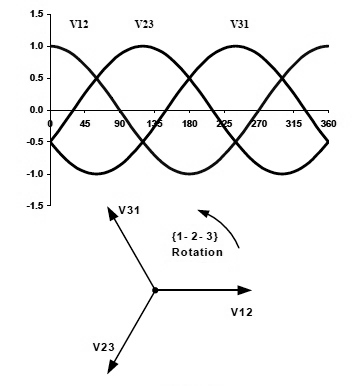
\includegraphics[width=\textwidth]{Unblance_EPS_Pics/Three-phase-voltage-system_gray.png}
         \caption{Three phase sine wave of network voltage.}
         \label{BASICUNB:fig:UnbWave}
     \end{subfigure}
		\hfill
     \begin{subfigure}[b]{0.49\textwidth}
         \centering
         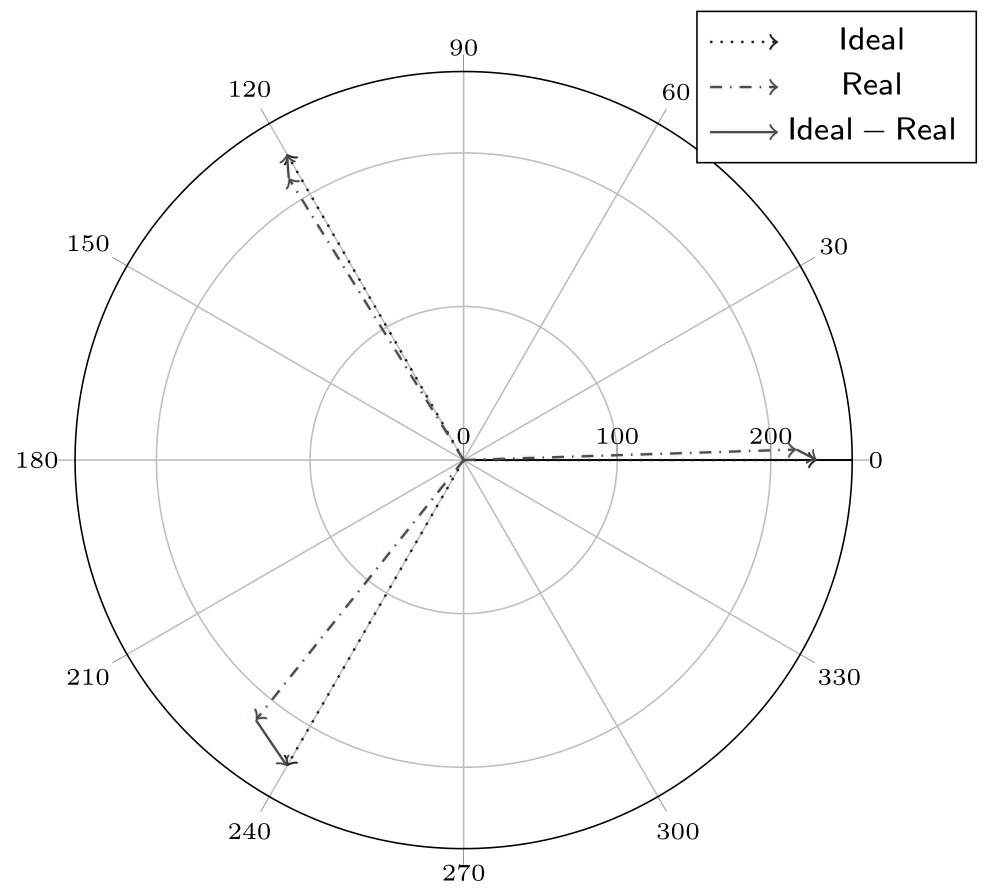
\includegraphics[width=\textwidth]{Unblance_EPS_Pics/PhasorGrayscale.jpg}
         \caption{The three phase voltage phasor whith $Ideal$ and $Real$ voltage vectors.}
         \label{BASICUNB:fig:UnbPhasor}
     \end{subfigure}
        %\caption{BASICUNB:fig:UnbPhasor}
        \label{BASICUNB:fig:UnbPhasor_all}
\end{figure}
	
	This is observed as a frequently cited power quality issue in low-voltage domestic distribution networks and in systems that supply large single phase loads distributed unevenly among the phases. Effects of voltage unbalance are complex, but can be categorized as structural or functional. The former refers to the asymmetry in the three-phase impedances of transmission lines, cables, transformers, etc. It occurs because it is neither economical nor necessary to maintain distribution system with perfectly symmetrical impedances. The latter refers to uneven distribution of power consumption over the three phases. Although the term voltage unbalance is unambiguous, the root phenomenon may be various as well as the standard norms used to measure unbalance. All of these different indicators measure voltage unbalance but each of them does it in a different way. In this section a detailed explanation is presented about the types of currently used method for indication.
	
	\subsection{Types of voltage deviations and norms}\label{BASICUNB:sec:DefinitionsofUNB}

        Voltage unbalance is not a straightforward term. To understand the concept, unbalance is when on a given frequency (mostly fundamental frequency) voltage vectors (phase or line depending on the definition) deviating from the ideal in terms of length or angle. The first fall in to the category of unbalance, namely any kind of phase deviations, and unbalanced amplitude deviations, and balanced amplitude deviations, like under-voltage. There are many different technological causes with more or less practical importance. The following conditions are examined and tested in the sequel:
        \begin{description}
        \item[Single phase under-voltage unbalance]  If there is a single phase uncompensated overload in the system, the voltage in the overloaded phase will be lower than the other two.
        \item[Two phase under-voltage unbalance]  Two of the three phases are overloaded without compensation, the two overloaded phases will have higher voltage drop than the third phase.
        Balanced three phase under-voltage]  The loads of all three phases are overloaded in an unbalanced manner.
        \item[Unbalanced single phase angle]  If the three phase voltage amplitudes are balanced but the relative angles between them (ideally it should be equal to $\pm120$ degree). It is assumed, that $V_a$ would be the reference. If one of the other two phase angles is deflected, unequal displacement.
        \item[Unbalanced two phase angles displacement] Similar to the single phase angle unbalance, if the other two phase angles are both deflected, then unequal angle displacement in two phase angles occurs.
        \end{description}
        An indicator of the voltage unbalance is supposed to measure the extent of unbalance but it is not expected to classify between the above types.
	
	\subsection{Non standardized approximation formulas}\label{BASICUNB:sec:ApproxFormula}
	
	Up to now, the following definitions have not been adopted by any standard or rule to indicate the degree of voltage unbalance, but used by various manufacturers. Firstly based on \cite{eugene1986new} recommended by the CIGRE (International Council on Large Electric Systems, in French: Conseil International des Grands Réseaux Électriques), the voltage unbalance is determined with:
	
	\begin{equation}
        \begin{array}{rcl}
            VUFactor&=&\frac{\sqrt{{1-\sqrt{3-6\frac{V_{ab}^4+V_{bc}^4+V_{ca}^4}{\left(V_{ab}^2+V_{bc}^2+V_{ca}^2\right)^2}}}}}{1+\sqrt{3-6\frac{V_{ab}^4+V_{bc}^4+V_{ca}^4}{\left(V_{ab}^2+V_{bc}^2+V_{ca}^2\right)^2}}}\\
						%\textnormal{where},&&\\
						%\upsilon&=&\frac{V_{ab}^4+V_{bc}^4+V_{ca}^4}{\left(V_{ab}^2+V_{bc}^2+V_{ca}^2\right)^2},					
        \end{array}
        \label{BASICUNB:equ:CIRGE}
    \end{equation}
		
		where, $\{V_{ab},V_{bc},V_{ca}\}$ are the line-to-line voltages. Note, that the CIRGE variant has no distinct notation, as such it would be indicated as $VUFactor$ in this thesis. Moreover, the author of \cite{robert1992assessing} recommends two more variants, based on manufacturer recommended"standards":
		
		\begin{equation}
        \begin{array}{rcl}
            VU&=&\frac{82\cdot\sqrt{(V_{ab}-V_{avg_{line}})^2+(V_{bc}-V_{avg_{line}})^2+(V_{ca}-V_{avg_{line}})^2}}{V_{avg_{line}}}\times100\\					
        \end{array}
        \label{BASICUNB:equ:VU}
    \end{equation}
		
		\begin{equation}
        \begin{array}{rcl}
            VUR&=&\frac{max\left( |V_{ab}-V_{bc}|,|V_{bc}-V_{ca}|,|V_{ca}-V_{ab}| \right)}{V_{avg_{line}}}\times100,\\				
        \end{array}
        \label{BASICUNB:equ:VUR}
    \end{equation}
		
		where the mean of line voltages is noted by $V_{avg_{line}}=\frac{V_{ab}+V_{bc}+V_{ca}}{3}$.
		This formulas were created with the intention to avoid the use of the complex algebra in symmetrical components and give
a good approximation of the later described $VUF$ standard. With the indicator of \ref{BASICUNB:equ:VU}, and as well as \ref{BASICUNB:equ:VUR}. It is worth noticing, that only the voltage magnitude unbalance is reflected, completely ignoring Fortescue's method of symmetrical components \cite{fortescue1918method} (shall presented later in the thesis), which considers negative sequence components as harmful on electric equipment and yield. Later it will be shown that other methods try to push the same methodology, until the currently used norm ($VUF$) is used.

	
	\subsection{LVUR}\label{BASICUNB:sec:LVUR}
	
	One of the first voltage unbalance in percent is defined by the National Electrical Manufacturers Association (NEMA) \cite{bonnett1997understanding} is defined  as the ratio of the maximum voltage deviation from the average line voltage magnitude to the average line-voltage magnitude.
	
\begin{equation}
        \begin{array}{rcl}
            LVUR&=&\frac{\max\left( |V_{ab}-V_{avg_{line}}|,|V_{bc}-V_{avg_{line}}|,|V_{ca}-V_{avg_{line}}| \right)}{V_{avg_{line}}}\times100\\			
        \end{array}
        \label{BASICUNB:equ:LVUR}
    \end{equation}
		
		The LVUR assumes that the average voltage is always equal to the rated value, which is 480 volts for the US three-phase systems, and it works only with magnitudes. Phase angles are not considered in this definition.
	
	\subsection{PVUR}\label{BASICUNB:sec:PVUR}
	
	The next phase voltage unbalance in percent described in IEEE standard $141.$ \cite{IEEE_141_35071} (derived from \cite{IEEE_112_8635630}), is $PVUR_{IEEE-141}$. It is defined as the ratio of the maximum voltage deviation of phase voltages from the average phase-voltage magnitude to the average phase voltage magnitude. In various fields, LVUR and $PVUR_{IEEE-141}$ are commonly used to estimate the degree of voltage unbalance due to simplicity of calculation. The two unbalance factors mentioned above cannot completely reflect system voltage unbalance effects, such as the phase displacements of unbalanced voltages.
	
	\begin{equation}
        \begin{array}{rcl}
            PVUR_{IEEE-141}&=&\frac{\max\left( |V_{a}-V_{avg_{phase}}|,|V_{b}-V_{avg_{phase}}|,|V_{c}-V_{avg_{phase}}| \right)}{V_{avg_{phase}}}\times100,\\
        \end{array}
        \label{BASICUNB:equ:PVUR-141}
    \end{equation}

where the voltages $\{V_{a},V_{b},V_{c}\}$ denotes the phase-to-neutral voltages, and $V_{avg_{phase}}=\frac{V_{a}+V_{b}+V_{c}}{3}$.
The second variant is, $PVUR_{IEEE-936}$, mentioned in \cite{IEEE_936_29053} is defined as the ratio of the difference between the highest and the lowest phase-voltage magnitude to the average phase-voltage magnitude. Therefore, the numerical values of voltage balance quantified by $PVUR_{IEEE-936}$ are generally larger than those of $PVUR_{IEEE-141}$ and LVUR.

\begin{equation}
        \begin{array}{rcl}
            PVUR_{IEEE-936}&=&\frac{\max\left( |V_a|,|V_b|,|V_c| \right)-min\left( |V_a|,|V_b|,|V_c| \right)}{V_{avg_{phase}}}\times100,\\					
        \end{array}
        \label{BASICUNB:equ:PVUR-936}
    \end{equation}
		
The number of possible combinations of three phase or line voltages that satisfy the definitions of voltage unbalance mentioned above will become infinite as only the magnitudes of voltages are considered.	
		
	
	\subsection{VUF and CVUF}\label{BASICUNB:sec:VUFCVUF}
	
	The voltage unbalance factor ($VUF$) was defined by the International Electrotechnical Commission \cite{pillay2001definitions}, \cite{dugan1996electrical}. From the theorem of symmetrical components \cite{fortescue1918method}, voltage unbalance can be considered as a phenomenon that positive sequence voltage  ($V_p$) is disturbed by negative  ($V_n$) and zero-sequence ($V_0$) voltages:
	
	\begin{equation}
        \begin{array}{rcl}
            \begin{bmatrix}
						V_0\\
						V_p\\
						V_n\\
						\end{bmatrix}&=&
						\frac{1}{3}\begin{bmatrix}
						1&1&1\\
						1&\upsilon&\upsilon^2\\
						1&\upsilon^2&\upsilon\\
						\end{bmatrix}\cdot
						\begin{bmatrix}
						V_a\\
						V_b\\
						V_c\\
						\end{bmatrix},\\
        \end{array}
        \label{BASICUNB:equ:symmetry}
    \end{equation}
	
	Where $\upsilon=e^{2j\pi/3}$ is the Fortesque operator. From that the formula of $VUF$ can be expressed as:
	
	
	\begin{equation}
        \begin{array}{rcl}
            VUF&=&\left|\frac{V_n}{V_p}\right|\times100,\\					
        \end{array}
        \label{BASICUNB:equ:VUF}
    \end{equation}

    \begin{figure}[h]
         \centering
         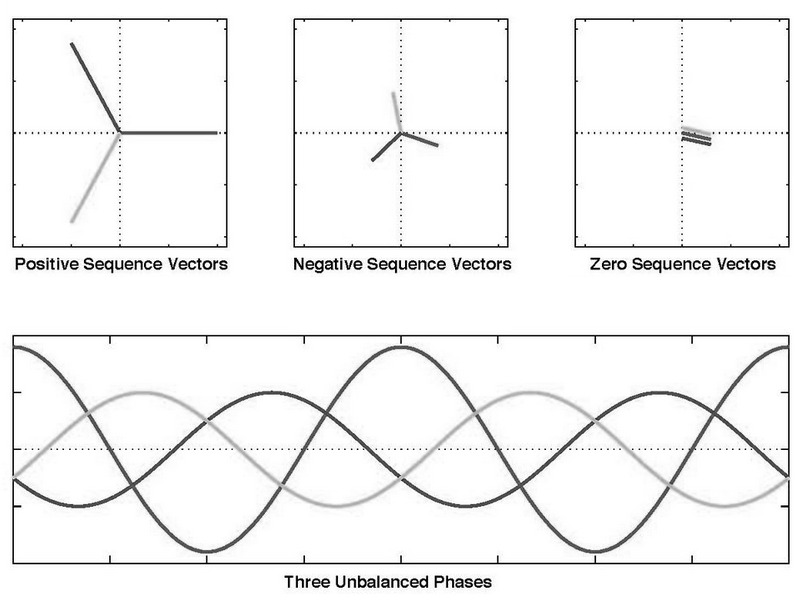
\includegraphics[width=.7\textwidth]{Unblance_EPS_Pics/Symmetrical_components_gray.jpg}
         \caption{Simplified graphical display of symmetrical components.}
         \label{BASICUNB:fig:symmetrical_simple}
     \end{figure}
	
This norm is currently in use world wide for voltage unbalance indication. The main focus in on the negative sequence component $V_n$, on which many studies attributes importance of the cause of negative effects the voltage unbalance causes.\\
	As such, three-phase electric loads without path through the neutral, negative-sequence voltage is the primary cause of voltage unbalance. Normally, positive-sequence component of three-phase voltages is very close to rated value. If expressed in per-unit quantities, the positive-sequence voltage will be very close to $1.0$ p.u., and the corresponding negative-sequence voltage will be very close to the $VUF$. Thus, the $VUF$ can indeed be considered as the negative-sequence component in per-unit.	This explains the advantage of using the VUF as an index for analyzing the effects of voltage unbalance considering the phase deviations.
	An extension of the VUF is the complex voltage unbalance factor ($CVUF$) that is defined by the ratio of the negative-
sequence voltage phasor to the positive-sequence voltage phasor studied in \cite{wang2000analytical}, and \cite{pierrat1987unbalance}. The CVUF is a complex quantity having the magnitude and the angle. Although the CVUF has not yet been widely used by practicing engineers, it has been proposed in some studies (e.g., \cite{wang2001analysis}, \cite{singh2007some}, \cite{chen2013examination}) due to its richness of information on unbalance. The formula of $CVUF$ is similar to $VUF$:

\begin{equation}
        \begin{array}{rcl}
            k_v&=&\frac{V_n}{V_p}=k_v\cdot e^{j\theta_v}=k_v\angle\theta_v,\\					
        \end{array}
        \label{BASICUNB:equ:CVUF}
    \end{equation}
		
		where $k_v$ is the magnitude and $\theta_v$ is the angle of $CVUF$.
		
			It can be observed, that the previously mentioned norms \ref{BASICUNB:equ:CIRGE}, \ref{BASICUNB:equ:VU}, \ref{BASICUNB:equ:VUR}, \ref{BASICUNB:equ:LVUR}, \ref{BASICUNB:equ:PVUR-141}, \ref{BASICUNB:equ:PVUR-936}, and \ref{BASICUNB:equ:VUF}  indicate different values for a single case with various correlations. The first two standard indicators, $PVUR_{IEEE-936}$ and $PVUR_{IEEE-141}$, ignore the $\pm120$ degree phase difference unbalance and only take the amplitudes into account. Additionaly, the zero-sequence components never present in the line-to-tine voltages regardless of the level of unbalance, only phase-to-neutral voltages. It has been proven, that these components are unelectable in some cases like bridge control of converters \cite{betz2006symmetry}, or synchronous machine diagnosis \cite{hang2015online}.\\
			The actual state of the art definition in use, $VUF$, is sensitive to the phase difference unbalance. Lastly $CVUF$ considers also phase and magnitude of the voltage unbalance, but the two units are hard to merge together as the optimization cost of a cost function. Moreover, these definitions ignore zero sequence components and harmonic distortion that are always present in three-phase four-wire systems \cite{bina2011three}.
		
% =========== SECTION MIGRATED TO INTRODUCTION -->

			%\section{Effects of voltage unbalance}
			%
			%Many power systems, voltage parameters change over time. Variation of power quality disturbances leads to thermal transients in electrical machines. This problem can be especially important in the case of low-power machines, because they have shorter time constants than high-power ones. The rate of thermal responses of a machine also significantly depends on the type of power quality disturbances. Voltage unbalance can cause  machine  overheating  within  a  mere  few  minutes. Furthermore,  fluctuating  unbalance  could  cause  an  extraordinary rise  in  windings  temperature  and  additional  thermo-mechanical stress.  Consequently,  voltage  unbalance  is  found  to  be  more harmful to induction motors than the results from previous works \cite{gnacinski2019induction}. Additionally beside the heat factor, voltage unbalance can cause increased reactive power \cite{savaghebi2012secondary}, various copper loss \cite{siddique2004effects} torque pulsation in electric motors \cite{brekken2005control} have been studied.

%	NO SUMMARY REQUIRED
	


\section{Basic notions for current source rectifier and EMPC}

	\subsection{Usage of current source rectifiers}

	\subsection{Basis of quadratic optimization and model predictive control}
	
	Predictive control methods based on a model are optimal regulators, with a defined cost function on a defined and encompassed  	prediction horizon with restrictions [N9], [N25], [N4], [N16], [N55]. The control signal is calculated over a defined horizon, but from the sequence of applicable control signals only the first one is used in the next sample. This procedure is repeated according to the principle of the moving horizon, using new iterations, as such provides the reaction in each sample. This method was developed for systems with physical restrictions, in the first stage for the control of chemical processes in the oil industry, then it was applied to various rapid processes from automotive or power electronics industry [N1] , [N13]. By default the optimization problem can be solved, for each sample, or explicitly using the multi-parameter programming techniques (mp-LP, mp-QP) presented in [N-ANNEX 1], over a well-defined parameter space.
	MPC example
	
	\subsubsection{Constained optimal control}
	
	Let the us assume that the system is linear and time-invariant (LTI):
	
	    \begin{equation}
        \begin{array}{rcl}
            x(t+1)&=&Ax(t)+Bu(t)\\
						y(t)&=&Cx(t)
        \end{array}
        \label{BASIC:equ:basic_LTI}
    \end{equation}
		
	with the restrictions:
	
	\begin{equation}
        \begin{array}{rcl}
            Ex(t)+Lu(t)\leq M\\
        \end{array}
        \label{BASIC:equ:restrict_LTI}
    \end{equation}
		
		where $t\geq0$ defines the time instance and $\textbf{x}\in \mathbb{R}^n$, $\textbf{u}\in \mathbb{R}^m$, $\textbf{y}\in \mathbb{R}^p$ are the states, inputs and uotputs of the system respectively. We define the following cost function to optimize:
		
		\begin{equation}
        \begin{array}{rcl}
				%&&\norm{asd}
         J(U_n,x(0))&=&\norm{{Px_N}}_p+\sum^{N-1}_{k=0}\norm{Qx_k}_p+\norm{Ru_k}_p\\
        \end{array}
        \label{BASIC:equ:cost_function}
    \end{equation}
		
		The optimization problem \ref{BASIC:equ:cost_function} applies with restrictions as follows:
		
		\begin{equation}
        \begin{array}{rcl}
				J^*(x(0))&=&min_{U_N}J(U_n,x(0))\\
					&&Ex_k+Luk\leq M,k=0,\dots,N-1\\
					&&x\in X_f\\
					&&x_{k+1}=Ax_k+Bu_k,k\geq0\\
					&&x_0=x(0)\\
        \end{array}
        \label{BASIC:equ:optim_problem}
    \end{equation}
		%
		where $N$ is the defined horizon, $x\in X_f$ is the set if terminal states, $U_N=[u_0,u_1,\dots,u_{N-1}]\in\mathbb{R}^s,s=m*N$. In case of $p=2$ (Euclidean norm) $Q=Q'\geq0$, $R=R'\geq0$, $P\geq0$ and in case of $p=1$, $Q$,$R$, and $P$ shall be on maximum rank.
		From \ref{BASIC:equ:cost_function} and \ref{BASIC:equ:optim_problem} a classical linear quadratic regulator (LQR) structure can be formulated with finite or infinite horison [N3], [N20], [N21].
		Let us consider the following:
		
		\begin{equation}
        \begin{array}{c}
         p=2, \left\{(x,u)\in\mathbb{R}^n+m:Ex+Lu\leq M\right\}=\mathbb{R},X_f=\mathbb{R}^n\\
        \end{array}
        \label{BASIC:equ:quadratic_case}
    \end{equation}
		
		In this case the problem can be reduced to an unconstrained optimization with finite horizon with the control law: 
		
		\begin{equation}
        \begin{array}{rcl}
         u^*(k)&=&K_kx(k), k=0,\dots,N-1\\
        \end{array}
        \label{BASIC:equ:control_law}
    \end{equation}
		
		Where the control coefficient of the $k^th$ instance is $K_k$ can be given in the following form:
		
		\begin{equation}
        \begin{array}{rcl}
         K_k&=&-(B'P_{k+1}B+R)^-1B'P_{k+1}A\\
        \end{array}
        \label{BASIC:equ:control_coefficient}
    \end{equation}
		
		The positive semi-definite matrix $P_k$ is the solution of the Riccati equation:
		
		\begin{equation}
        \begin{array}{rcl}
        P_N&=&P\\
				P_k&=&A'(P_{k+1}-P{k+1}B(B'P_{k+1}B+R)^-1B'P_{k+1})A+Q\\
        \end{array}
        \label{BASIC:equ:Riccati}
    \end{equation}
		
		whith the initial condition:
		
		\begin{equation}
        \begin{array}{rcl}
				J^*(x(0))&=&x(0)'P_0x(0)\\
        \end{array}
        \label{BASIC:equ:Riccati_initial}
    \end{equation}
		
		If we choose $N\longrightarrow\infty$ and assume that $(A,B)$ are controllable and $(A,B)$ are observable, the optimization problem becomes an infinite horizon LQR whose solution can be written as:
		
		\begin{equation}
        \begin{array}{rcl}
         u^*(k)&=&K_kx(k), k=0,\dots,\infty\\
        \end{array}
        \label{BASIC:equ:control_law_infinite}
    \end{equation}
		
		As such:
		
		\begin{equation}
        \begin{array}{rcl}
         K_k&=&-(B'P_\infty B+R)^-1B'P_\infty A\\
        \end{array}
        \label{BASIC:equ:control_coefficient_infinite}
    \end{equation}
		
		with P as the unique solution of the Riccati equiation:
		
		\begin{equation}
        \begin{array}{rcl}
				P_\infty&=&A'(P_\infty-P\infty B(B'P_\infty B+R)^-1B'P_\infty)A+Q\\
        \end{array}
        \label{BASIC:equ:Riccati_infinite}
    \end{equation}
		
		These are the basis of model predictive control (MPC). For introduction let us consider the principle of moving horizon (Receding Horizon). Optimization over a finite horizon has the following disadvantages:
		
		\begin{itemize}
			\item Unforeseen problems may occur after the fixed optimization horizon, which may cancel the sequence of order for the 		calculated finished horizon.
		\item After reaching the time defined by the horizon, the law of command is no longer optimal.
		\item Finite horizon optimization is usually used because of the limited computing power is available, and not for theoretical reasons 
		\end{itemize}
		
		To prevent this problem, the notion of optimization is introduced on a moving horizon. In each sample $k$ , an optimization problem is solved over a defined horizon $k,\dots,k+N$ to calculate the appropriate command sequence, and only the first command is applied. This results in a moving optimization horizon, which eliminates the issues listed before. The Formulation of the optimal control problem with moving horizon [N14] in the system \ref{BASIC:equ:basic_LTI} with input and output constraints follows:
		
		\begin{equation}
        \begin{array}{c}
				y_{min}\leq y(t)\leq y_{max},u_{min}\leq u(t)\leq u_{max},\\
        \end{array}
        \label{BASIC:equ:receiding_horison_constraints}
    \end{equation}
		
		
with the cost function to minimize:
		
		\begin{equation}
        \begin{array}{rcl}
				J(U,x(t)&=&x'_{t+N_y|t}Px_{t+N_y|t}+\sum^{N_y-1}_{k=0}x'_{t+k|t}Qx_{t+k|t}+u'_{t+k}Ru_{t+k},\\
				&&y_{min}\leq y_{t+k|t}\leq y_{max},k=1,\dots,N_c-1,\\
				&&u_{min}\leq u_{t+k}\leq u_{max},k=0,1,\dots,N_c-1,\\
				&&x_{t|t}=x(t),\\
				&&x_{t+k+1|t}=Ax_{t+k|t}+Bu_{t+k},\\
				&&y_{t+k|t}=Cx_{t+k|t}, k\geq0,\\
				&&u_{t+k}=-Kx_{t+k|t}, N_u\leq k\leq N_y,\\
        \end{array}
        \label{BASIC:equ:receiding_horison_problem}
    \end{equation}
		
		where $Q=Q'\geq0$, $R=R'\geq0$, $P\geq0$, $(C,A)$ is observable, [missing text] and $N_u\leq N_y$, $N_c\leq N_y-1$. One trivial possibility to choose $K=0$ and $P$ to satisfy the Lyapunov equation:
		
		\begin{equation}
        \begin{array}{rcl}
				P&=&A'PA+Q\\
        \end{array}
        \label{BASIC:equ:receiding_horison_Lyapunov}
    \end{equation}
		
		This means that after $N_u$ samples the control stops and the system is evolving to an open loop form. It is obvious that the choice only makes sense if the open loop system is stable. The second option would as described in \ref{BASIC:equ:control_coefficient_infinite}, and \ref{BASIC:equ:Riccati_infinite}, but this involves to use an unconstrained control for $N_u$ LQR samples. As a result, the MPC law calculates the optimal command sequence:
		
		\begin{equation}
        \begin{array}{rcl}
				U^*(t)&=&\left\{u^*_t,\dots,u^*_{t+N_u-1}\right\},\\
        \end{array}
        \label{BASIC:equ:receiding_optimal_sequence}
    \end{equation}
		
		and only the first control input is applied:
		
		\begin{equation}
        \begin{array}{rcl}
				u(t)=u^*_t.\\
        \end{array}
        \label{BASIC:equ:receiding_optimal_first}
    \end{equation}
		
		The optimal control inputs estimated for future samples are not taken into account and the algorithm is
repeated on the basis of new measurements or a new estimation of the states.

\subsubsection{Stablilty of MPC}		
		
			%\item 
		%\end{itemize}

	\subsection{Formulating explicit model predictive control structures}
	
	asd





\section*{Notations used in the chapter}

\begin{scriptsize}
\begin{tabularx}{\textwidth}{r|X}


	$\hat{V}$															& Voltage peak\\
	$\vec{V}_a, \vec{V}_b, \vec{V}_c,$										& Voltage vectors in the three phase phasor\\
  $VUFactor,VU,VUR$                	& Non standardized voltage unbalance factor based on manufacturer standards\\
	$V_{ab},V_{bc},V_{ca}$  					& Line-to-line voltages\\
	$V_{avg_{line}}$  								& Average of line voltages\\
	$LVUR$														& Voltage unbalance notation based on NEMA standard\\
	$PVUR_{IEEE-141},PVUR_{IEEE-936}$	& Voltage unbalance notation based on IEEE-141, and IEEE-936 standard\\
	$V_{a},V_{b},V_{c}$  							& Phase-to-neutral voltages\\
	$V_{avg_{phase}}$  								& Average of phase voltages\\
	$V_{0},V_{p},V_{n}$  							& Zero, negative and positive sequence voltages based on symmetrical components theorem\\
  $\upsilon$  											& Fortesque operator\\
	$VUF$  														& Voltage Unbalance Factor\\
	$CVUF$  													& Complex Voltage Unbalance Factor\\
	$k_v$  														& Magnitude of CVUF\\
	$\theta_v$  											& Angle of CVUF\\
	$i_i$															& Constant input inductor current\\
	$i_o$															& Alternating output current\\
	$V_i$															& Constant input voltage\\
	$V_o$															& Alternating output voltage\\
	$L_+,L_-$													& Current filter inductors\\
	$S_{1+},S_{2+}$										& Higher switches\\
	$S_{1+},S_{2+}$										& Lower switches\\
	$D_{1+},D_{2+}$										& Higher diodes\\
	$D_{1+},D_{2+}$										& Lower diodes\\
	$V_{an},V_{bn}$  									& Designated point's potential to ground \\
	$\omega$													& Angular velocity of output sinusoidal voltage or current\\
	$V_{D1},V_{D2}$ 									& Two end's voltage on the DC-DC converter\\
	$v_1,v_2$                         & Transformer voltages\\
	$C_{snub}$ 												& Capacitance to reduce switching loss and to damp out over-voltage\\
	$n$ 															& Transformer turn ratio.\\
	$L_a$															& Leakage inductance\\
	$v_D$															& Output voltage before the choke inductor $L_D$\\
	$V_d$															& Output voltage\\
	$I_D$															& Output current\\
	$L_D$															& Inductor for filtering the output current of the CSR (Choke)\\
	$C_D$															& Capacitance for filtering the output voltage of the VSR\\
	$L_S$															& Input filter inductance of the three phase alternating current in VSR\\
	$C_S$															& Input filter capacitance of the three phase alternating current in CSR\\
	$v_{c_p}$													& AC-side capacitor voltage, where $p\in\{1,2,3\}$\\
	$\widehat{u}$											& Peak value of AC-side capacitor voltage\\
	$v_{i,j}$													& Three phase phase-to-neutral voltage $i,j\in\{R,S,T\}$\\
	$v_{N,RS}$												& Three phase line-to-line voltage of $R$ and $S$\\
	$\varphi_N$												& Angle of phase voltage\\
	$\vec{i}$													& Rectifier input current\\
	$\vec{i}_ref$											& Reference rectifier input current\\
	$x$																& State of a linear time invariant model\\
	$f(x)$														& Function of the state\\
	$\rho$																& Infinite sequence iterator\\
	$\Delta$													& Step lenght control parameter\\
	$\mathcal{P},\mathcal{D},\mathcal{S},\mathcal{Q},\mathcal{U},\mathcal{I},\mathcal{E}$ & Set of processes, directions, succesful iterations, timestep index, internal successes, and external successes respectively\\
	$p$																& Process number\\
	$i$																& Active process indicator\\
	$d_i$															& Direction of active process\\
	$x_i^{best}$											& Best reached state, where $x_i^{best}$ is a minima\\
	$\Delta_i^{best}$											& Best reached step size\\
	$q$																& Discrete time step\\
	$\omega_i(q)$ 										& Generating process index for the update time at step $q$ on process $i$\\
	$\tau_i(q)$												& Time index for initialization of the function evaluation, that produced the update at time $q$ on process $i$\\
	$\nu_i(q)$ 												& Time index for the completion of the function evaluation that produced the update at time step $q$ on process $i$\\



	$\textbf{A}$																& State matrix of a linear time invariant model\\
	$\textbf{B}$																& Input matrix of a linear time invariant model\\
	$\textbf{C}$																& Output matrix of a linear time invariant model\\
	$\textbf{x}$											& State vector of a linear time invariant model\\
	$\textbf{z}$											& Input vector of a linear time invariant model\\
$s$                             & Dimension of the decision vector\\
$m$                             & Dimension of the input vector\\
$n$                             & Dimension of the state vector\\
$J_0$                           & Cost function to optimize at the initial state\\
$\textbf{x}(0)$                 & Initial state\\

	$\textbf{P}$                    & Terminal penalising weight matrix\\
$\textbf{Q}$                    & State penalising weight matrix\\
$\textbf{R}$                    & Input penalising weight matrix\\

	$N$											& Defined horizon of MPC\\
	$N_c,N_u,N_y$											& Defined control, input, and output horizon respectively\\
	$k$																& Time step on the horizon $N$ \\

$\mathcal{X}^x$             & Set of all possible future states stepping through the horizon\\
$\mathcal{S}^x$             & Set of all possible future state matrices stepping through the horizon\\
$\mathcal{S}^u$             & Set of all possible future input matrices stepping through the horizon\\
$\textbf{H}$, $\textbf{F}$, $\textbf{Y}$ & Supplementary matrices\\
$\textbf{U}^*_0$            & Optimal vector of future inputs starting from the initial state\\
$J^*_0$            & Optimal cost value at the initial state\\
$j$                         & Intermediate step index on the horizon\\
$\mathcal{U}^u$             & Set of inputs not violating constraints\\
$\textbf{A}_x$              & Constraint state matrix\\
$\textbf{b}_x$              & Constraint state coefficient\\
$\textbf{A}_u$              & Constraint input matrix\\
$\textbf{b}_u$              & Constraint input coefficient\\
$\textbf{A}_f$              & Constraint state matrix at the end of the horizon\\
$\textbf{b}_f$              & Constraint state coefficient at the end of the horizon\\
$\mathcal{P}$               & Set of all (input and state) constraints at time instance\\
$\textbf{G}$                & Unified constraint input matrix \\
$\textbf{E}$                & Unified constraint state matrix \\
$\textbf{W}$                & Unified constraint coefficient matrix \\
$\tilde{\textbf{z}}$        & Set of all future states and inputs over the horizon\\
$\textbf{z}$                & Optimal controller evolution vector over the horizon\\
$\textbf{K}$                & Controller gain\\
$g$                         & Autonomous function where there are no inputs\\
$V$                         & Lyapunov function\\

\end{tabularx}
\end{scriptsize}




%% Voltage Unbalance
\chapter[Voltage unbalance compensation]{Voltage unbalance compensation with optimization based control algorithm and asymmetrical inverter structure}\label{VUB:sec:Main}

In this section a new approach shall be discussed around the phenomena of voltage unbalance in a small domestic network. First the networks structure shall be described, the power electrical system is connected to, as a household supplying, renewable untilising device. Then a control cost-function candidate, the proposed geometrical approach shall be presented, as an indicator of voltage unbalance. Finally, the aforementioned device's topology and control shall be presented based on the geometrical voltage unbalance norm, with the performance results on an unbalanced network.
		
\section{Network structure}\label{VUB:sec:Network}

         The examined network is supposed to be the low voltage local transformer area with regular households, depicted in Figure \ref{fig:network}. The network structure of Figure \ref{fig:network} has been implemented in Simulink\texttrademark\, environment for simulation based experiments. Most of the households represent a single phase load with resistive inductive and capacitive properties while some of them are symmetric three phase ones. There might also be some households with domestic power plant, they are not only loads but also represents distributed generators. Furthermore, it is assumed that the households located on a domestic size grid tie inverter are also provided with battery storage capacities. Commercially available inverters are capable of optimizing the working point and charging current of the system, while the ability of power quality improvement is far not typical - it is in experimental phase in some cases, e.g. \cite{gorbe2012reduction}.%

        \begin{figure}[!ht]
            \centering
            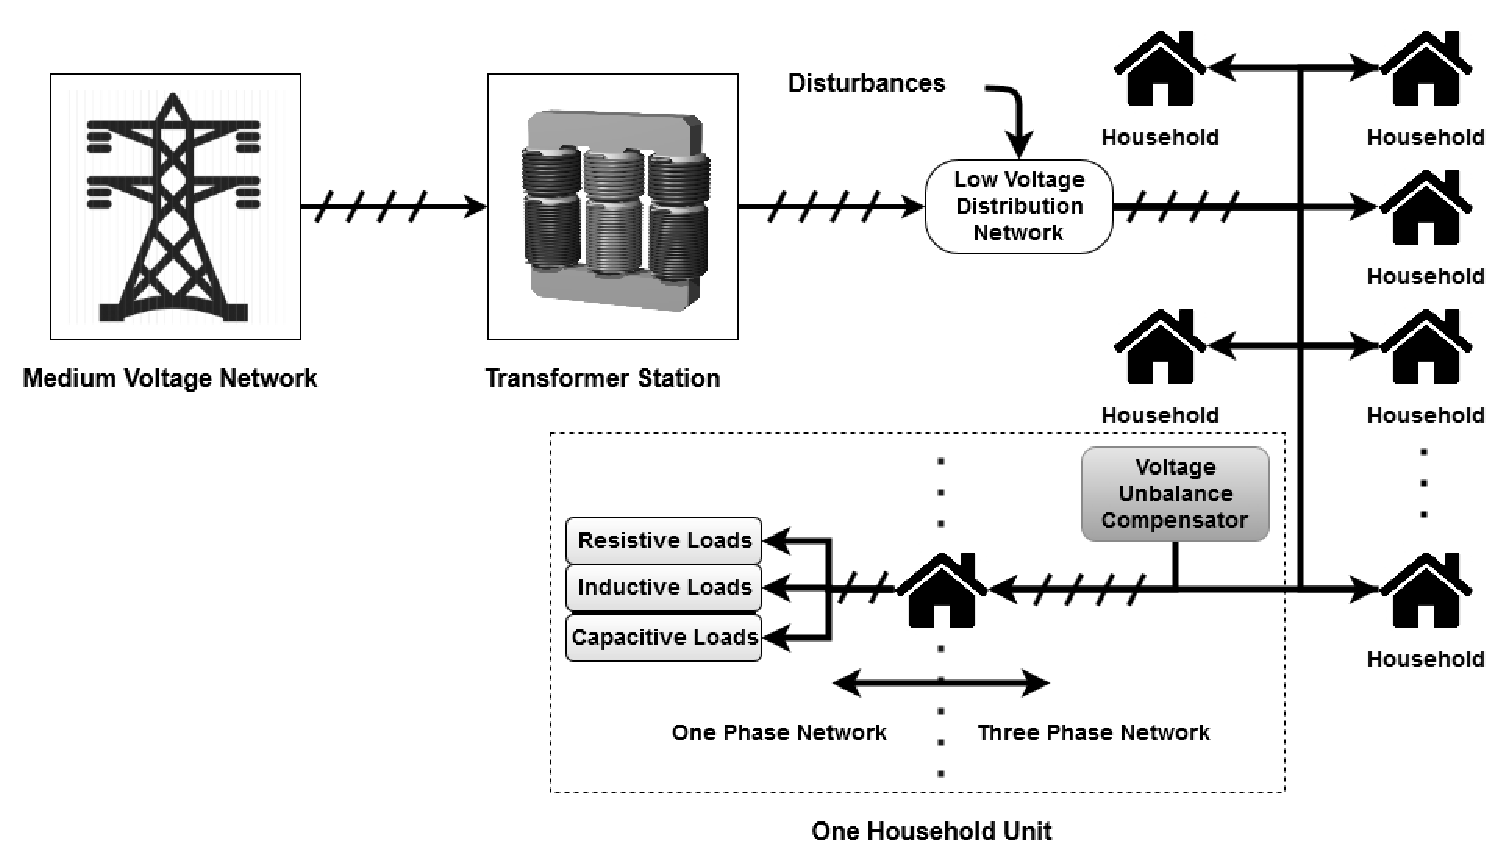
\includegraphics[width=\textwidth]{Unblance_EPS_Pics/network_gray.eps}
            \caption{The simplified structure of a three phase four wire low voltage network. The transformer station acts as transition from the medium voltage power grid to
            the low voltage network. The several regular households are representing the main loads of the network. The transformer and the loads are connected with power line sections infected by inductive and resistive disturbances and capacitive couplings. Domestic powerplants can connect to any connection point within the low voltage network, via an appropriate inverter - either to the three phase sections using a three phase inverter or to a single phase using a single phase inverter.}
            \label{fig:network}
            \end{figure}
        
\section{Proposed geometrical indicator}\label{VUB:sec:Geom}

    As discussed in section \ref{BASICUNB:sec:DefinitionsofUNB}, the indicators of voltage unbalance result very different measures for the same circumstance. Additionally most of them neglecting the phase differences of voltage vectors compared to the ideal, and even the currently used $VUF$ calculated by \ref{BASICUNB:equ:VUF} is not taking zero sequence components from the Foresque method \cite{fortescue1918method}. There were attepts to close the gap with the CVUF norm shown in \ref{BASICUNB:equ:CVUF}, where the complex component is also considered, but this makes this a clumsy candidate for control design, since two components (real and complex part) shall weighted and applied. This begs the question, how could voltage unbalance be measured loss-less, but resulting one (conveniently quadratic-like) value, easyli applicable for minimization algorithm \\
		Hence can be stated that every difference between the ideal and the measured voltage in both amplitude phase and sub-harmonics causing a form of voltage deviation. The problem can also be investigated from a geometrical point of view as it is depicted in Figure \ref{fig:threephase}. The three-phase voltage system's phasor diagram contains three  phase-to-neutral voltage vectors which can be regarded as the points of a triangle (similarly, the three line-to-line vectors can play the role of the edges of the triangle). The two triangles (i.e. the ideal and the actual ones) always intersect except from very extreme and physically meaningless cases. The area where the two triangles do not cover each other (i.e. the difference of their union and intersection) can be used as a norm of voltage quality. In fact it is computationally more demanding compared to the previous methods, but takes every deviation into consideration \cite{Neukirchner2015},\cite{neukirchner2015examination}. The calculation of error is given by (\ref{equ:geom}).

            \begin{equation}
                \begin{array}{rcl}
                       G&=&\textnormal{Area of }(\bigtriangleup_{Ideal}\cup\bigtriangleup_{Real}-\bigtriangleup_{Ideal}\cap\bigtriangleup_{Real}),
                \end{array}
                \label{equ:geom}
            \end{equation}

            $\bigtriangleup_{Ideal}$ indicates the triangle spanned by the ideal voltage vectors and $\bigtriangleup_{Real}$ the triangle of real voltage vectors. Difference of the ideal and the real triangle's union and intersection defines the norm $G$. Basically, the algorithm calculates the symmetrical difference of the triangles, stretched from three phase ideal and real voltage vectors.

            \begin{figure}[!ht]
           \centering
           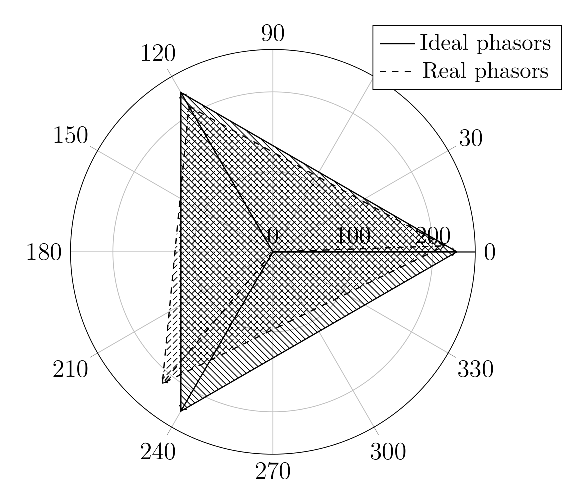
\includegraphics[scale=0.95]{Unblance_EPS_Pics/UnbalRedComp_JCP-figure1.eps}
           \caption{The triangles spanned by the ideal and the actual voltage phasors. The extent of voltage deviation on the network can be measured by the sum of areas where the two triangles are not overlapping.}
           \label{fig:threephase}
            \end{figure}

\section{The method's additional content compared to VUF}\label{VUB:sec:AdditionalContent}

When using a new method for calculation and cost function it is reasonable to test it's usability against the prevalent or regulated method the voltage unbalance factor ($VUF$) defined by the International Electrotechnical Commission, as discussed in section \ref{BASICUNB:sec:VUFCVUF}. In this case the geometrical norm's utility (\ref{equ:geom}) against the $VUF$ (\ref{equ:regular}) value shall be examined. \\
The geometrical norm was validated experimentally, by investigating the correlation between the regulated (\ref{equ:regular})  and geometrical (\ref{equ:geom}) norms subjected to random, uniformly distributed unbalance on the voltage vector amplitude and phase values with $20$ V amplitude and $1/300\cdot\pi$ rad phase variance (Fig. \ref{fig:correlation}, and Fig. \ref{fig:side_correlation}).

            \begin{figure}[!ht]
           \centering
           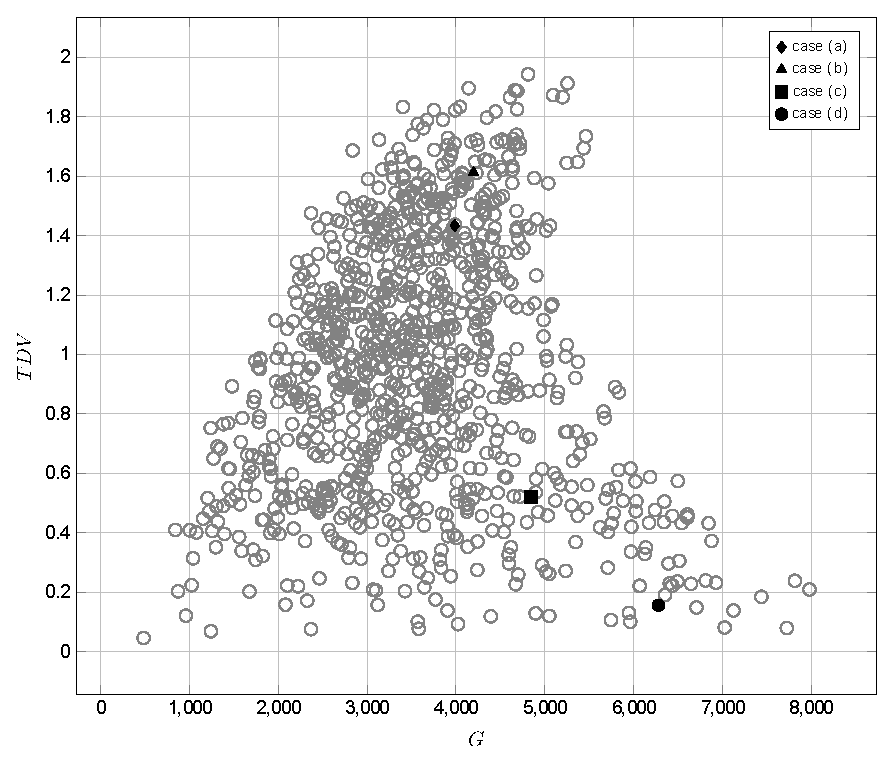
\includegraphics[width=\textwidth,scale=0.95]{Unblance_EPS_Pics/EPS_images/scatter.eps}
           \caption{Correlation between the geometrical voltage unbalance indicator $G$ and the regulated voltage unbalance indicator $TDV$ using 1000 samples. In every iteration each three phase voltage vector's amplitude and phase values changed randomly, according to uniform distributions with $\pm20$ V and $\pm\frac{1}{3}\pi\cdot10^{-2}$ rad variance. It can be seen, that the geometric norm contains more information than the classical one. The  four asymmetry cases of Figure \ref{fig:cases} are denoted by black symbols on the picture. It is apparent, that in case (c), and (d) the G norm holds additional information than the TDV.}
           \label{fig:correlation}
            \end{figure}

            \begin{figure}[!ht]
           \centering
           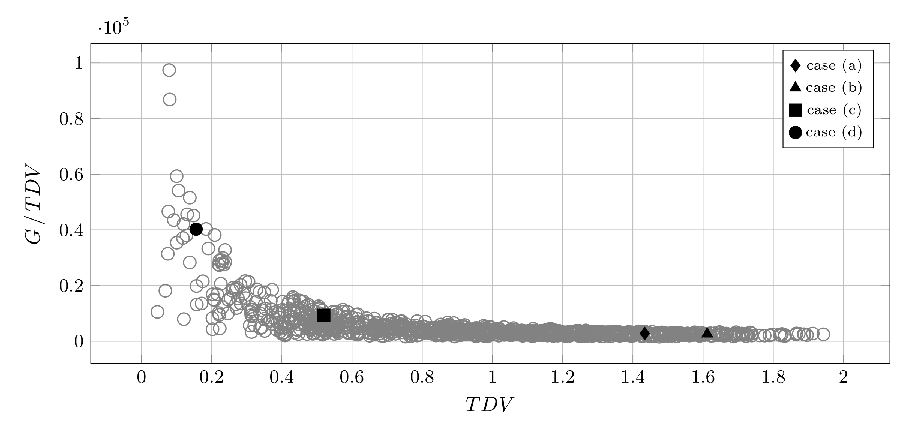
\includegraphics[width=\textwidth,scale=0.95]{Unblance_EPS_Pics/EPS_images/side_scatter.eps}
           \caption{\textbf{Itt a .eps converzio nem lett valami jo, javitani kell!} Correlation between the regulated unbalance indicator and the fraction of geometrical and regulated indicator. It can be seen that there is a functional connection between the two values.}
           \label{fig:side_correlation}
            \end{figure}


            Although there is correlation between the two norm values in the general case, but for some situations the regular method indicates low, while geometrical norm still indicates high value.\\
            On Figure \ref{fig:cases_A} dominant phase deviation can be observed, while Figure \ref{fig:cases_B} shows amplitude deviation but with opposite direction. When there is such deviation on the grid both indicators present almost identical results. On \ref{fig:cases_C} there is still observable unbalance (two phase deviate stronger than the third in terms of amplitude), but the correlation is significantly lower. In the last case in the lowest correlation area, amplitude deviation is present, but the deviation direction is identical on all phases (balanced over-voltage or under-voltage)(Figure \ref{fig:cases_D}). The regular method indicates very low values. In this case other methods are utilised in parallel in terms of network diagnostics to detect the under-voltage phenomena.\cite{arn1997under-voltage}.


            \begin{figure}
                \centering
                \begin{subfigure}[b]{0.48\textwidth}
                    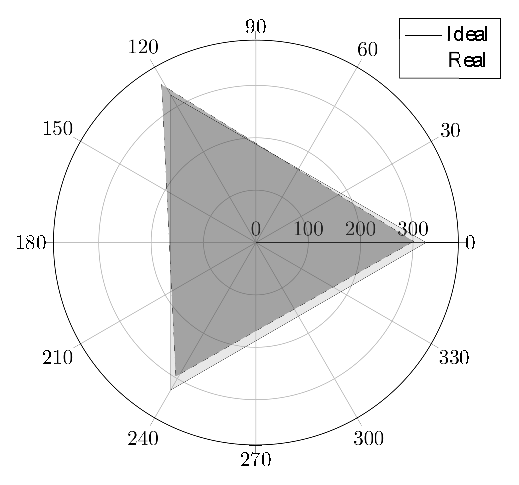
\includegraphics[width=\textwidth]{Unblance_EPS_Pics/EPS_images/rombus.eps}
                    \caption{\centering High correlation with phase deviation. The norm values are $G=3986$ and $TDV=1.434$.}
                    \label{fig:cases_A}
                \end{subfigure}
                ~ %add desired spacing between images, e. g. ~, \quad, \qquad, \hfill etc.
                  %(or a blank line to force the subfigure onto a new line)
                \begin{subfigure}[b]{0.48\textwidth}
                    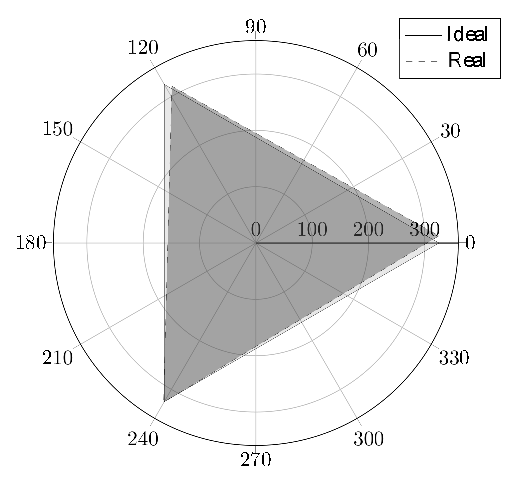
\includegraphics[width=\textwidth]{Unblance_EPS_Pics/EPS_images/triangle.eps}
                    \caption{\centering High correlation with opposed amplitude deviation. The norm values are $G=4198$ and $TDV=1.612$.}
                    \label{fig:cases_B}
                \end{subfigure}
                 %add desired spacing between images, e. g. ~, \quad, \qquad, \hfill etc.
                %(or a blank line to force the subfigure onto a new line)
                \begin{subfigure}[b]{0.48\textwidth}
                    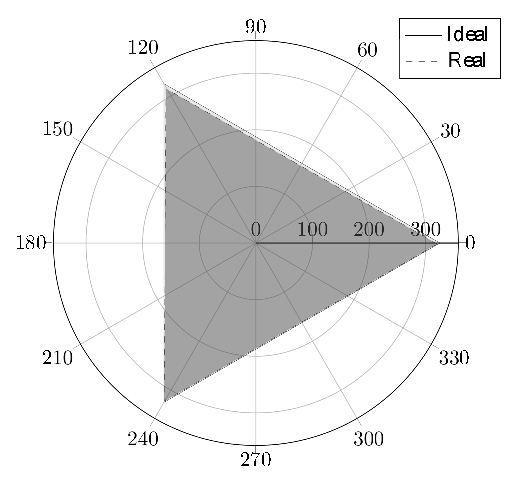
\includegraphics[width=\textwidth]{Unblance_EPS_Pics/EPS_images/square.eps}
                    \caption{Low correlation with opposed amplitude deviation. The norm values are $G=9322$ and $TDV=0.5198$.}
                    \label{fig:cases_C}
                \end{subfigure}
                ~
                \begin{subfigure}[b]{0.48\textwidth}
                    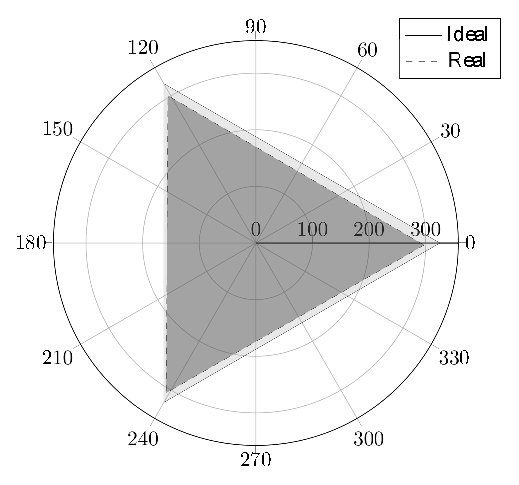
\includegraphics[width=\textwidth]{Unblance_EPS_Pics/EPS_images/circle.eps}
                    \caption{\centering Low correlation with uniform voltage drop. The norm values are $G=6280$ and $TDV=0.156$.}
                    \label{fig:cases_D}
                \end{subfigure}


                \caption{Four distinct cases of voltage triangles examining correlation between the regular $TDV$ and geometrical $G$ method.}\label{fig:cases}
            \end{figure}

To clarify this, the regular norm's calculation method needs to be investigated. The symmetrical component mutual impedance matrix on a three phase connection point is given by (\ref{equ:mutual}),

            \begin{equation}
                \begin{array}{rcl}
                       Z_s&=&\frac{1}{3}\begin{bmatrix} 1&1&1\\1&\alpha&\alpha^2\\1&\alpha^2&\alpha \end{bmatrix}\cdot
                                        \begin{bmatrix} Z_{aa}&Z_{ab}&Z_{ac}\\Z_{ba}&Z_{bb}&Z_{bc}\\Z_{ca}&Z_{cb}&Z_{cc} \end{bmatrix}\cdot
                                        \begin{bmatrix} 1&1&1\\1&\alpha^2&\alpha\\1&\alpha&\alpha^2\end{bmatrix}=\\
                          &=&  \begin{bmatrix} Z_{00}&Z_{01}&Z_{02}\\Z_{10}&Z_{11}&Z_{12}\\Z_{20}&Z_{21}&Z_{22} \end{bmatrix},

                \end{array}
                \label{equ:mutual}
            \end{equation}

where $Z_s$ is the symmetrical component mutual impedance matrix, and $\alpha=e^{j\frac{2}{3}\pi}$. If there are both negative and zero sequence symmetrical components present on the network, the dominant part of the voltage drop's negative and zero sequence can be calculated as follows (\ref{equ:drop}).

            \begin{equation}
                \begin{array}{rcl}
                       \Delta U_2&\approx&Z_{21}I_1+Z_{22}I_2\\
                       \Delta U_0&\approx&Z_{01}I_1+Z_{00}I_0,
                \end{array}
                \label{equ:drop}
            \end{equation}

$\Delta U_0,\,\Delta U_1,\,\Delta U_2$ are the voltage drop's zero positive and negative sequence components, $I_0,\,I_1,\,I_2$ are the current's drop's zero positive and negative sequence components, and $Z_{00},Z_{01},\,Z_{21},\,Z_{22}$ are mutual impedances,  respectively. (If there is only positive and negative sequence present, then the right hand side's second term is zero.) As such, the indication of negative and zero sequence present the network calculates (\ref{equ:factor}):

            \begin{equation}
                \begin{array}{rcl}
                       m_{21}&=&\mid\frac{Z_{21}}{Z_{11}}\mid\times100\\
                       m_{01}&=&\mid\frac{Z_{01}}{Z_{11}}\mid\times100,
                \end{array}
                \label{equ:factor}
            \end{equation}

where $m_{21}$ is the negative sequence factor which is identical to the TDV (\ref{equ:regular}), and $m_{01}$ is the zero sequence factor.\\
At the previously described balanced over- or under-voltage case the positive sequence value is dominant, so the regular indicator will take considerably lower value. In other words, aside from indicating voltage unbalance, the geometrical method incorporates the balanced deviations as well. In a control design perspective, a general case, where notably highly unbalance values may appear, using $TDV$ as cost function could introduce hidden errors in control due error cancellation. Additionally the geometrical solution checks electrical asymmetry, i.e. the norm of a $\pm120$ degree rotated version of the ideal three-phase phasor is zero in the geometrical sense. Moreover, the geometrical norm is more sensitive for small scale unbalance, as opposed to the TDV. To summarize, the geometrical indicator a more suitable solution for a more general case indicator, and a good candidate for cost function in optimal control design.

\section{Unbalance compensation}\label{VUB:sec:Compensation}

Based on the proposed measures on voltage unbalance indication, it is possible to formulate some power quality related aims, or demands for the domestic size generator units implemented in a complex power electrical system, capable of supplying a household, with both renewable and network supplied energy, and lowering voltage unbalance as well.

\subsection{Problem statement}\label{VUB:sec:Statement}

    The voltage and current unbalance presents in the three phase low voltage transformer area causes additional power loss inside the medium voltage/low voltage transformer and in the transportation line wires too. It also has undesired effects in certain three phase loads, mainly rotating machines where it causes torque reduction and pulsating torque effect. Large scale unbalance can activate automatic protection functions of electricity dispatch system causes power outage. This is unpleasant for the customers and adds maintenance cost to the service provider. These negative effects lower the electric power quality and rises the cost of electrical energy and rises the carbon footprint of our everyday life. The paper's aim to propose a model and control for a three phase instrumentation, which can compensate these undesirable effects, lower or eliminate the voltage and current unbalance to lower the power losses and the CO${}_2$ emission and increase power quality not only at the connection point but in the whole low voltage transformer area. \emph{It is important to note, that this power quality improvement can be achieved without any significant added cost.} The future aim is to integrate this function into an existing three phase photovoltaic inverter device connected to the low voltage grid, and a  complex energetic system is able to inject the renewable energy to the transportation network, can store the electrical energy from stochastic renewable sources in electrical vehicle batteries or feed the grid from the charged batteries in energy deficit and high demand simultaneous situations. Our new added value is the integrated control algorithm which can highly lower or eliminate the observed unbalance of the network.

    \subsection{Control problem}\label{VUB:sec:Control}

    The above problem statement partially specifies the solution space together with the solution method. The system of interest is the power grid with all the stochastic and nonlinear phenomena present in it mentioned in section \ref{VUB:sec:Network}. The input to the system are current signals (one current in the single phase case and three in the three phase setup), which are naturally constrained by the available energy of the household, stored in a battery pack or momentarily generated by the wind or solar generator unit. The response of the system can be either the current or the voltage measured at the connection point of the inverter unit, however, the general legal regulations only allow voltage measurement for consumers. The difficulty of the control problem comes from the fact, that there are no mathematically tractable models of the network can be generated because of its unpredictable and nonlinear features. This means, that in these therms only black-box methods can be applied for this system.
For the control aim it is a natural choice to minimize the actual voltage unbalance of the low voltage local transformer area measured (or calculated) at the connection point of the inverter. Several optimization based methods are available for such kind of optimal control problems, e.g. \cite{gorbe2012reduction} where the only bottleneck is the computational efficiency since the implemented controller has to run on the commercial inverter's hardware (digital signal processor unit).

    \subsubsection{Asymmetrical inverter structure}\label{VUB:sec:Inverter}

    For the sake of completeness an asymmetrical inverter was developed in simulation environment, which is capable of carrying out the specified control task. The renewable energy injection is realized increasingly, and applied directly to the three phase low voltage grid  with a domestic size photovoltaic power plant as source of power. This can reduce the voltage and current unbalance caused by the stochastic power production of wind and solar sources. More and more manufacturers produce three phase grid synchronized inverters from 5\,kW size. These equipments implement accurate symmetrical current feed with a standard three phase full bridge structure, consists of six Isolated Gate Bipolar Transistors (IGBT). The demand is to employ a current source single phase structure with aforementioned controllable switches in section \ref{BASICCSR:sec:CSI}. This is a standard structure suitable for symmetric harmonic current injection. It has limited capacities to inject not totally symmetric 3 phase current time functions, but Kirchhoff's current law permits only constant zero-sum current time functions injected with this structure. There are examples with this type of asymmetric current injections in the literature \cite{lee2009new}.\\
    This type of current injections has limited compensation capacity and this is not enough in most asymmetric production and load cases. In our case we need more general, not specific asymmetric current waveforms, because the proposed control aim assumes the ability of injecting non zero-sum currents. This needs special inverter design structure. We need zero line connection for the differential current. One of the possible solution is to use 3 different full bridge single phase current inverters to supply each phase of low voltage transportation lines \cite{Patnaik2013topologies}. This way it is most sufficient to use bi-directional power flow, with galvanic decoupling, but with a current controlled fashion (shown in section \ref{BASICCSR:sec:CSI}).\\
    This isolation can be reached  with using isolation transformers in the supply side. But we prefer to use it a complex energetic system with specific inside true DC bus system fed from Photovoltaic panel or batteries. We have to isolate at least 2 full bridges with two way DC-DC converters (described in section \label{BASICCSR:sec:DCDC}). This can complicate the physical realization but easy to simulate with two controlled power source. Other possible easy to realize solution to isolate the full bridge outputs  connected to three phase lines with isolating transformers. It is recommended due to electric shock protection reasons. Our distant aim to compensate other operational type line failures, such zero current appearing. This isolation method doesn't allow to produce DC current components, thats why we are looking for other design. Possible elegant solution to supplement the standard three phase inverter design with a fourth half bridge for Zero line, building a specific four leg inverter design \cite{Ninad2014control}.\\
    Only drawback of this solution is the complex difficult control method of the half bridges, to keep the current sum in zero values in each moment, and to provide the correct current paths inside the inverter. This structure has the lowest production cost, but in the phase of proofing the asymmetry compensation we chose the DC-DC isolated  full bridge design for simulation purpose because of the simple control during simulation.\\
    As a further generalization step, the injection of no harmonic current shapes will be necessary in order to decrease the extant Total Harmonic Distortion (THD) of the network. These expectations yield an inverter with new structure suitable for arbitrary current injections without limitations. The design lends similar elements like in \cite{gorbe2012reduction} by means of battery charge, renewable power point tracking, intermediate voltage, and IGBT bridge control, but in this case the problem requires a three phase solution for the voltage unbalance reduction. The applied structure based on a full bridge IGBT structure used in single phase current injection. Three different IGBT full bridge were connected at the output point, thus our structure has three phase and neutral connection too, to carry out any current form. The disadvantage of this structure is that it needs 12 IGBTs in the output stage as opposed to the 6 IGBTs needed for a classical full bridge structure and needs three galvanically isolated direct current (DC) voltage source for feeding.\\
    The other standard elements, that the inverter design consists:

        \begin{itemize}
            \item Standard maximum power point tracking (MPPT) input stage, to inject the maximum available power from the renewable source to the intermediate voltage capacitor with a simple controlled boost converter
            \item A half bridge current controller to charge or deploy the battery pack connected to the complex energetic system for energy storage and energy unbalance compensation
            \item Intermediate voltage controller
            \item Universal three phase output stage with 3 single phase full bridge IGBT current injector and 2 high current DC-DC converter
        \end{itemize}
    This is suitable to inject any necessary current shape to the low voltage three phase grid connection even DC currents too. Later a power loss and production cost analysis will be necessary if the built structure will be suitable for asymmetric compensation of low voltage transformer area.

        %\begin{figure*}[ht]
%            \centering
%            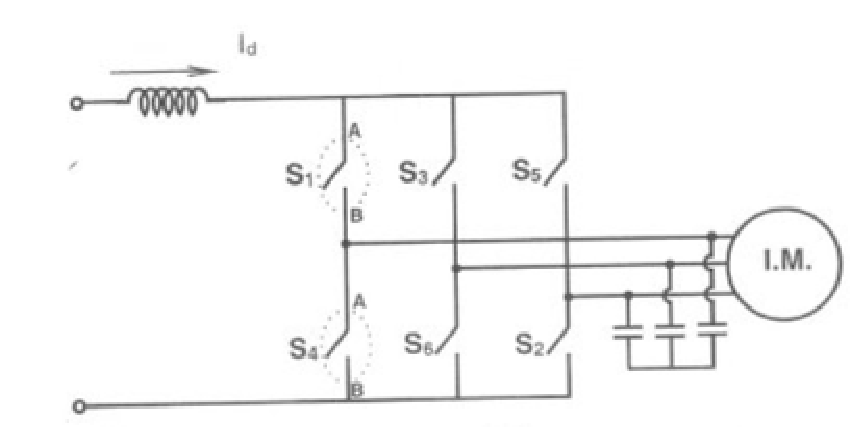
\includegraphics[width=0.95\textwidth]{standard_inverter.eps}
%            \caption{\textcolor{blue}{Standard symmetrical current inverter design, implies 6 IGBT current injector with serial inductance. }}
%        \label{fig: symminv}
%        \end{figure*}

        %\begin{figure*}[ht]
%            \centering
%            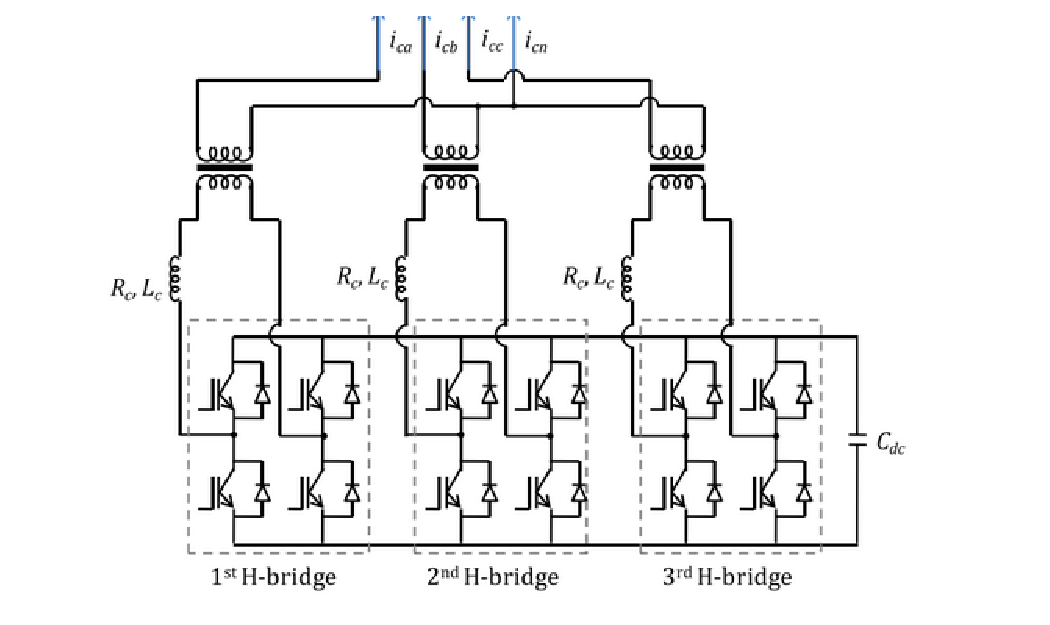
\includegraphics[width=0.95\textwidth]{isolated_inverter.eps}
%            \caption{\textcolor{blue}{Asymmetrical inverter design with three separated H-bridges.}}
%        \label{fig: asymminvwithDCgalvanic transformer}
%        \end{figure*}
%
%\begin{figure}[h]
%          \begin{center}
%                \begin{circuitikz}[scale=.5, european] %% => Itt ne állíts a skálát, inkább a figure-nél!%%
%                %\draw[help lines] (0,0) grid (16,40);
%
%                \draw%[color=magenta]
%                    %% híd
%                    (0,0) to[C=$C_{intermediate}$] (0,38)
%                    (0,0) to[short] (10,0)
%                    (6,0) node[nigbt, anchor=E](nigbt33){}
%                    (nigbt33.E) node[circ]{}
%
%                    (10,8) node[nigbt, anchor=E,xscale=-1](nigbt32){}
%
%                    (6,8) node[nigbt, anchor=E](nigbt31){}
%                    (nigbt33.C) to[short] (nigbt31.E)
%
%                    (10,0) node[nigbt, anchor=E, xscale=-1](nigbt34){}
%                    (nigbt34.C) to[short] (nigbt32.E)
%
%                    (nigbt32.C) to[short] (10,12)
%                    (nigbt31.C) to[short,-*] (6,12)
%                    (4,12) to[short] (10,12)
%                    (4,12) to[short,-*] (4,38)
%
%
%                    %%trafó
%                    (7,6) node[transformer,rotate=90,transform shape,american](T3){}
%                    (T3.B1) to[short,-*] (6,7.05)
%                    (T3.B2) to[short,-*] (10,7.05)
%                    (T3.A1) to[short] (7,4)
%                    (7,4) to[short,-o] (13,4) node[anchor=west] {$N$}
%                    (T3.A2) to[short,-o] (13,4.95) node[anchor=west] {$T$}
%                    ;
%
%                    \draw%[color=blue]
%                    %% híd
%                    (3,13) to[short,*-] (10,13)
%                    (6,13) node[nigbt, anchor=E](nigbt23){}
%                    (nigbt23.E) node[circ]{}
%
%                    (10,21) node[nigbt, anchor=E,xscale=-1](nigbt22){}
%
%                    (6,21) node[nigbt, anchor=E](nigbt21){}
%                    (nigbt23.C) to[short] (nigbt21.E)
%
%                    (10,13) node[nigbt, anchor=E, xscale=-1](nigbt24){}
%                    (nigbt24.C) to[short] (nigbt22.E)
%
%                    (nigbt22.C) to[short] (10,25)
%                    (nigbt21.C) to[short,-*] (6,25)
%                    (4,25) to[short,*-] (10,25)
%
%
%
%
%                    %%trafó
%                    (7,19) node[transformer,rotate=90,transform shape,american](T2){}
%                    (T2.B1) to[short,-*] (6,20.05)
%                    (T2.B2) to[short,-*] (10,20.05)
%                    (T2.A1) to[short] (7,17)
%                    (7,17) to[short,-*] (12,17)
%                    (T2.A2) to[short,-o] (13,17.95) node[anchor=west] {$S$}
%                    ;
%
%                    \draw%[color=cyan]
%                    %% híd
%                    (3,26) to[short] (10,26)
%                    (3,26) to[short,-*] (3,0)
%
%                    (6,26) node[nigbt, anchor=E](nigbt13){}
%                    (nigbt13.E) node[circ]{}
%
%                    (10,34) node[nigbt, anchor=E,xscale=-1](nigbt12){}
%
%                    (6,34) node[nigbt, anchor=E](nigbt11){}
%                    (nigbt13.C) to[short] (nigbt11.E)
%
%                    (10,26) node[nigbt, anchor=E, xscale=-1](nigbt14){}
%                    (nigbt14.C) to[short] (nigbt12.E)
%
%                    (nigbt12.C) to[short] (10,38)
%                    (nigbt11.C) to[short,-*] (6,38)
%                    (0,38) to[short] (10,38)
%
%
%                    %%trafó
%                    (7,32) node[transformer,rotate=90,transform shape,american](T1){}
%                    (T1.B1) to[short,-*] (6,33.05)
%                    (T1.B2) to[short,-*] (10,33.05)
%                    (T1.A1) to[short] (7,30)
%                    (7,30) to[short] (12,30)
%                    (12,30) to[short,-*] (12,4)
%                    (T1.A2) to[short,-o] (13,30.95) node[anchor=west] {$R$}
%                    ;
%                %%
%                \end{circuitikz}
%                \caption{Simplified asymmetrical inverter design employing three galvanically isolated H-bridges with transformers for DC-DC isolation substitution.}
%                \label{fig: asymminvwithgalvanic transformer}
%          \end{center}
%        \end{figure}

        \begin{figure*}[ht]
        \centering
        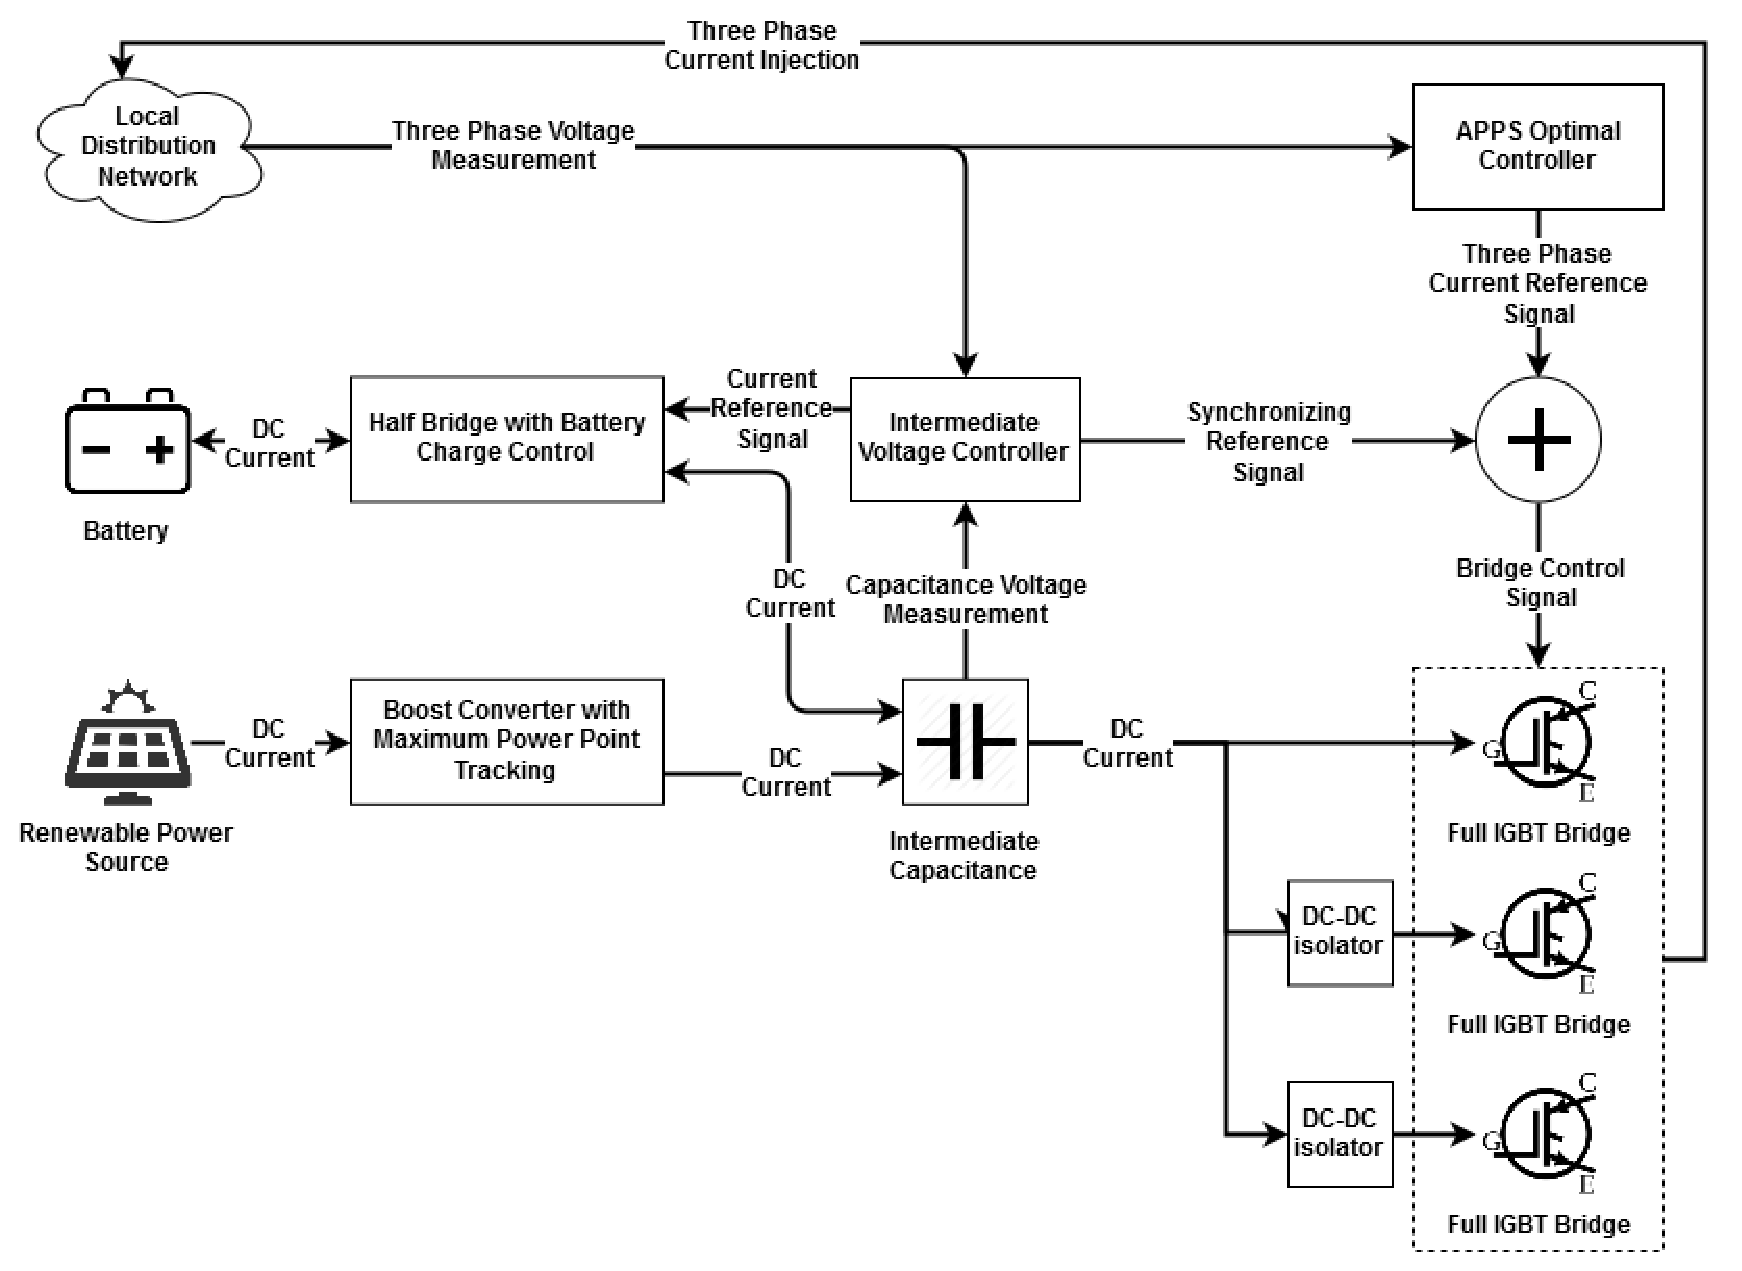
\includegraphics[width=0.95\textwidth]{Unblance_EPS_Pics/inverter.eps}
        \caption{The asymmetrical inverter design, which applies three single phase full bridge IGBT current injector to create the injected asymmetrical current shapes for voltage unbalance compensation. }
        \label{fig:inv}
        \end{figure*}

        Of course there is a possibility that there is no renewable power available for a longer period of time and the battery completely looses its charge. In this case the system should work merely with the power of the connection point but with zero energy balance. This states to operate two controller with semi-opposite control goals. The optimization based controller requires current injection while the intermediate voltage controller (Figure \ref{fig:inv}) keeps the inverters energy balance. Although for this operation some of the control's performance should be sacrificed, unbalance compensation could be achieved even without external renewable power, and energy storage at a minimum power requirement.

        \subsubsection{Measurements from a real unbalanced network}\label{VUB:sec:Measurement}

            The measurements took place at the Faculty's building, where a common 400\,V connection point was investigated as the behaviour of the network. The three phase 230\,V line-to-ground voltages has been transformed to 6\,V to be effectively measurable time domain with high performance NI-USB DAQ on 10\,ksample/s. Because of the limited computational capacity only a 10 second measurement was made in every hour.  The measurements then has been merged and smoothed to eliminate the inter-measurement transients.\\
            Afterwards, the measurement data has been used as the input of a micro-grid segment of the Matlab/Simulink model, to test the controller and inverters structure's performance in quasi-realistic circumstances. The controllers performance on the simulated microgrid's network loss reduction can be observed on Figure \ref{fig:compare_power} and Figure \ref{fig:u_inter}. The measurement output is connected to a modeled three phase load and network system, consisting of symmetrical loads and network segments between them. Further artificial load unbalance is not necessary since the network's unbalance is already present. This structure enables to show that any point the inverter is connected could serve as quality restoration such unbalance compensation at this case. Our future plan is to set up multiple devices on different connection points.

    \subsection{Optimization based control algorithm}\label{VUB:sec:Optimization}

        \begin{figure*}[ht]
        \centering
        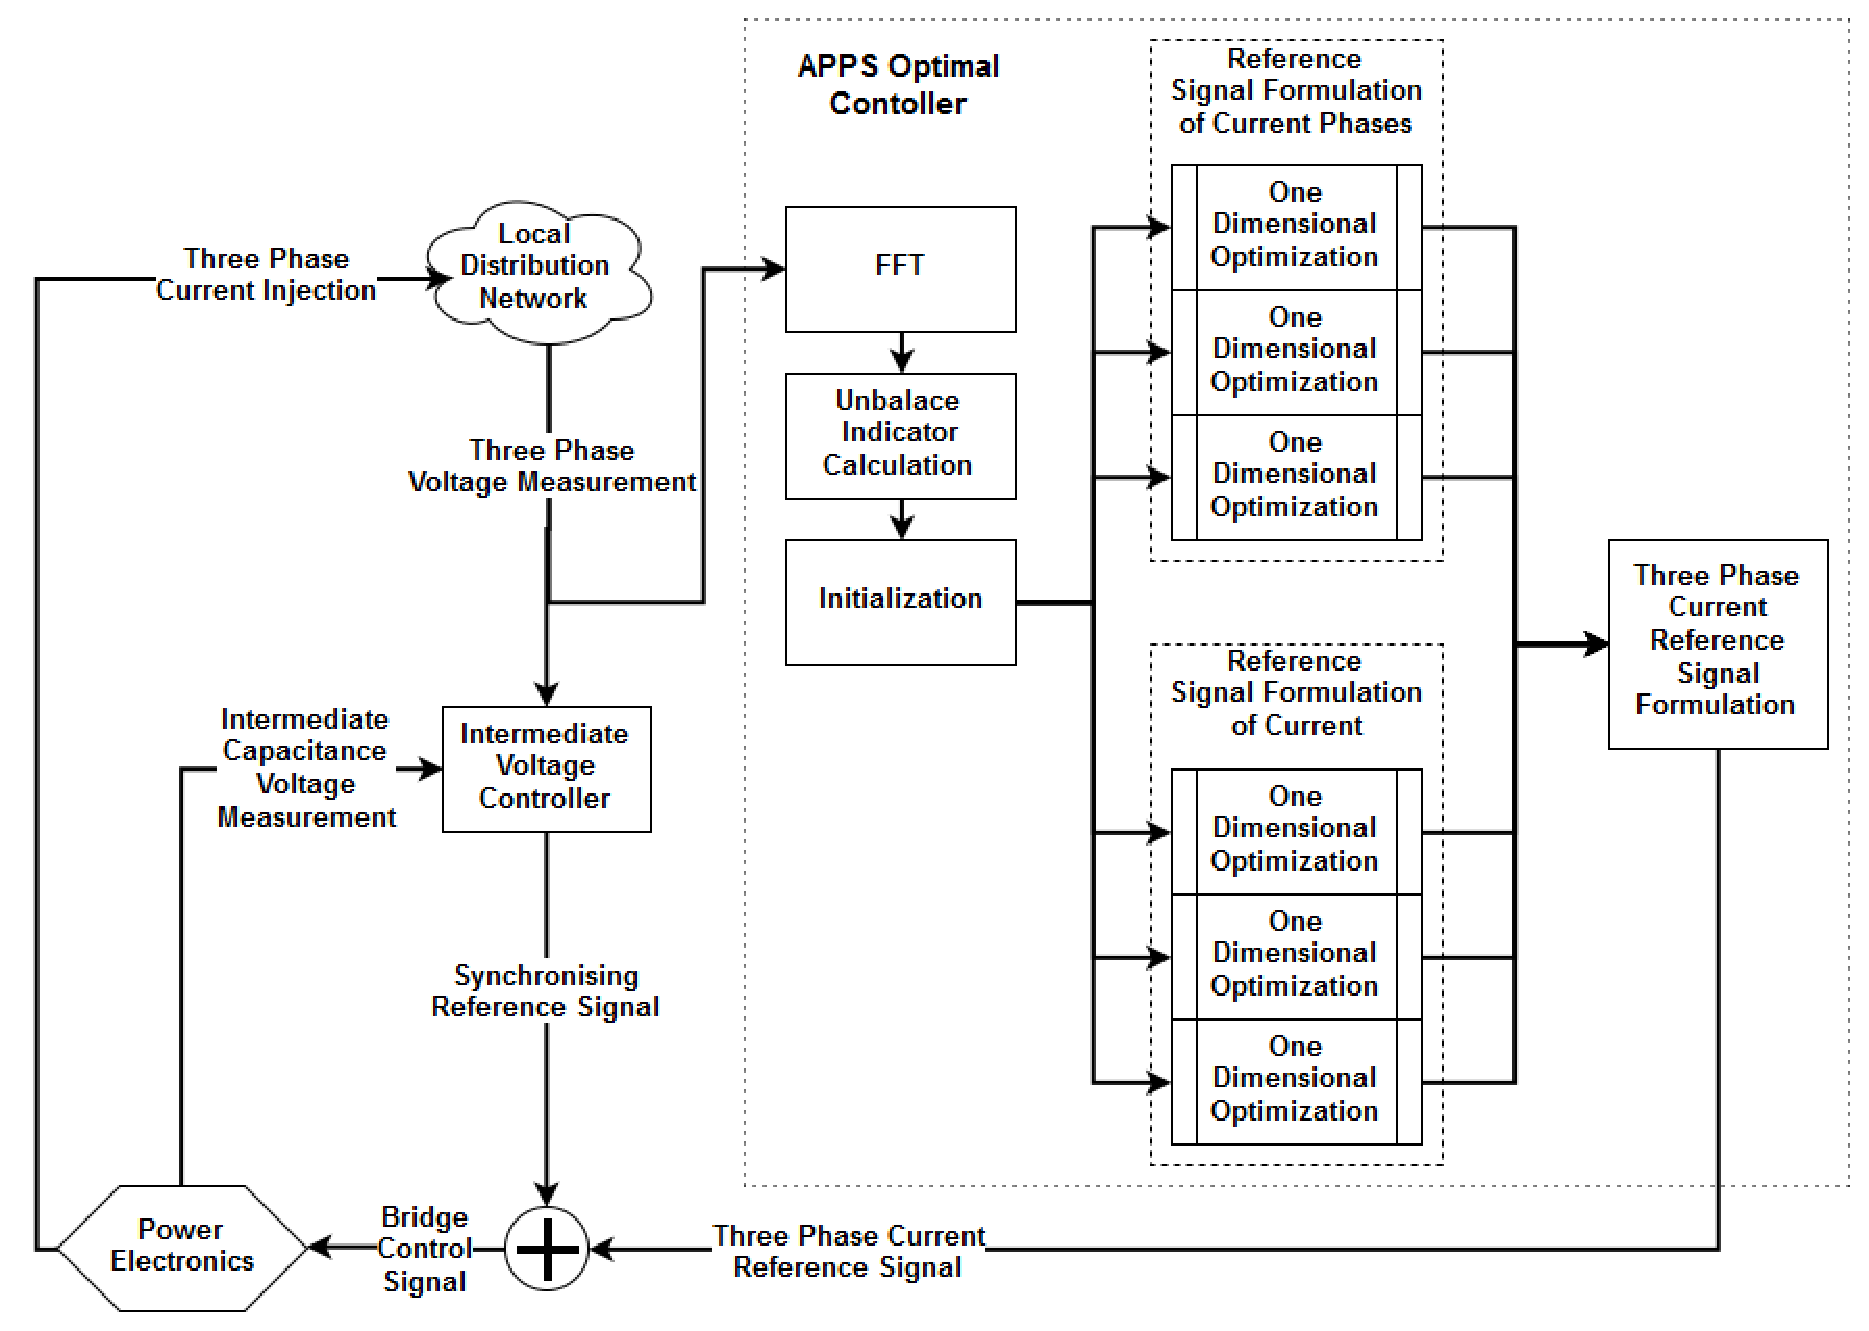
\includegraphics[width=0.95\textwidth]{Unblance_EPS_Pics/APPS_1_2_.eps}
        \caption{The optimization algorithm implemented for current control. A one dimensional linear optimization step is being solved in each dimension of the six dimensional parameter space, iteratively.}
        \label{fig:APPS}
        \end{figure*}

        The problem is that, the exact mathematical relation is nonlinear because the nonlinear, and highly time variant loads of the network, we should use a control strategy to cope this nonlinear and time variant energy system. For this purpose we chose an asynchronous parallel pattern search method (APPS) which could be able to control our scenario \cite{hough2001asynchronous}. The methodology and formulation of the APPS method is described in section \ref{BASICUNB:sec:APPS}. We applied a variant of the gradient method that is a first-order optimization (minimization) algorithm for a multivariate function $f(x)$. The point $x(q)$ corresponding to the local minimum can be calculated from the negative gradient $\nabla f(x)$, that gives the value and direction of the corresponding step in the parameter space. The next step is made in the direction of gradient with the proper sign. This sequence of steps, ideally, converges to local multivariate extreme value $x(q)$ of the function (\ref{eqn:contstruct1}).

        \begin{equation}
        \begin{array}{rcl}
        \label{eqn:contstruct1}
         x^{(q)}&=&x^{(q-1)}-t_q\nabla f(x^{(q-1)}),\\
         %q&\in&\mathbb{N},\\
         \end{array}
        \end{equation}

        where $q\in\mathbb{N}$, and $t_q$ resembles the step time of the algorithm. The controlled electrical system is described by multivariate non-linear differential equations, the optimization of which is infeasible to derive using the differentiation of an error function. Therefore, the optimization methods based on direct differentiation are not applicable. In such cases, when high computational power is needed for performing long time-consuming simulations, the APPS method can utilized. The search pattern $p$ is based on the sampling of the error function (selected norm) on a "grid", and it corresponds to variables or subsets of variables in each point in the independent variable or parameter space easily. At the same time, the norm values at these points can be calculated independently if $\Delta_q>0$, using (\ref{eqn:contstruct2}).
				
        \begin{equation}
        \label{eqn:contstruct2}
        \begin{array}{rcl}
         x^{(q+1)}&=&x^{(q)}+\Delta_qd_i \\
         \mathrm{if}&&f(x^{(k)}+\Delta_qd_i) \leq f(x^{(q)}),\\
         %q&\in&\mathbb{N}\\
         \end{array}
        \end{equation}

        The parameter is $x(q)\in\mathbb{R}^n$, and the search pattern $p\in\mathcal{D}={d_1,...d_n}$ is taken from a predefined finite set. In this case, the error function values should be calculated for each pattern $p$ in the set $D$. If the error function is not decreasing in any of the directions, then the step size should be reduced (e.g. by half). As the competing directions are different, if there is not enough computing power available for direction vector $p$, synchronization should not be maintained. In this case we are talking about the asynchronous case . In the case of our controller, an individual $p$ vector is defined for each output variable, and the optimization was performed in each direction asynchronously and shifted in time. Most likely, the error function has a single local minimum as a symmetric amplitude and phase values. Approaching the minimal value of norm, the controller uses adaptive increments that are proportional to the norm itself. Because of the complex interactions between the components of the controller, only one parameter is changed at a time, even if the values of the amplitude and phase components in specific time slot changes. The algorithm moves along the six axes of six separate time slots close to the local minimum of the error function.\\
        Unlike other similar approaches, e.g. \cite{segui2007approach}, the explained optimal controller does not rely on a measured current signal (which varies according where the measurement took place on the grid and renders the global optimization unreliable) but rather measuring and analyzing the voltage unbalance via the proposed indicator and optimizes the voltage shape, the latter of which depends on the nonlinear distortion of the whole low-voltage transformer area and determines additional power losses. The controller's performance was compared to a non compensated network, and a network consisting synchronized symmetric power intake from a regular inverter.\\
        In each iteration only one physical value is changing on the six dimensional parameter field, which consists of the three amplitude and three phase values. If the change effects with cost function reduction (the reference norm's normalized value), the controller holds the new value of amplitude or phase for the controlled current sources (Figure \ref{fig:APPS}). The advantage of this controller structure that is not necessary to know the controlled value's behavior well, like we could not determine the number and type of the other loads on the network \cite{Neukirchner2015}. There are however two disadvantages. First is the low speed of control, due to the several necessary iterations (depending on the circumstances) to find the optimal directions in the parameter space, and the serial nature of interventions and norm calculations. The second comes from the method itself since the controller may stuck in local minima.

\section{Discussion}\label{VUB:sec:Discussion}

write stuff here..

    \subsection{Dynamical simulation based experiments}\label{VUB:sec:Results}
		
		\textbf{Simulation's PC parametes, ML/Simuling version}\\
\\
    In order to be able to investigate the proposed optimization based unbalance reduction control structure with the three phase inverter on a low voltage local grid, all the elements of this complex electrical system (including the photovoltaic source, the inverter, the battery and the nonlinear local grid with different types of loads) has been modeled in Matlab/Simulink environment. The primary aim of the simulation based experiments were to serve as a proof of concept for the proposed complex control structure.

    \subsection{Performance analysis}\label{VUB:sec:Performance}

    The aim of performance analysis is twofold. First of all, the proposed voltage unbalance indicator has to be investigated in the control structure as the cost function of the optimization based controller, and on the other hand, the control structure itself has to be exposed against engineering expectations.


            The results of the first experiment can be seen in Figure \ref{fig:compare_asym_PV} where the geometrical norm \ref{equ:geom} has been used as the voltage unbalance indicator and the cost function for the optimizer.  The dashed line represents the examined low voltage local network's unbalance norm ($G$) without the proposed controller implemented in the inverter unit of the domestic powerplant while the solid line represents the compensated network's norm value. The performance of the controller with this norm is apparent, it was able to decrease the network voltage unbalance by approximately 85 \%. In this experimental setup the controller has enough input energy due to the batteries and the available solar power.

            \begin{figure*}[ht]
            \centering
            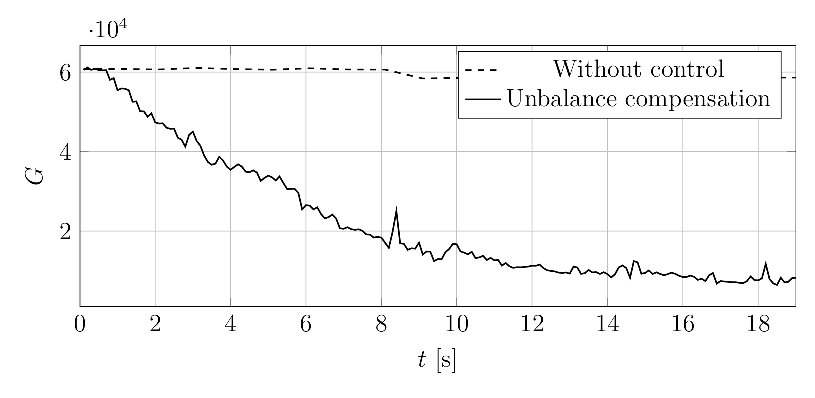
\includegraphics[width=0.95\textwidth]{Unblance_EPS_Pics/UnbalRedComp_JCP-figure3.eps}
            \caption{Unbalance reduction control system performance with half charged battery and photovoltaic power source available. The underlying unbalance norm is the geometrical one ($G$) in this experiment. After starting the controller at $t=0.1s$ the unbalance measure $G$ of the network significantly decrease.}
            \label{fig:compare_asym_PV}
            \end{figure*}

            \begin{figure*}[ht]
            \centering
            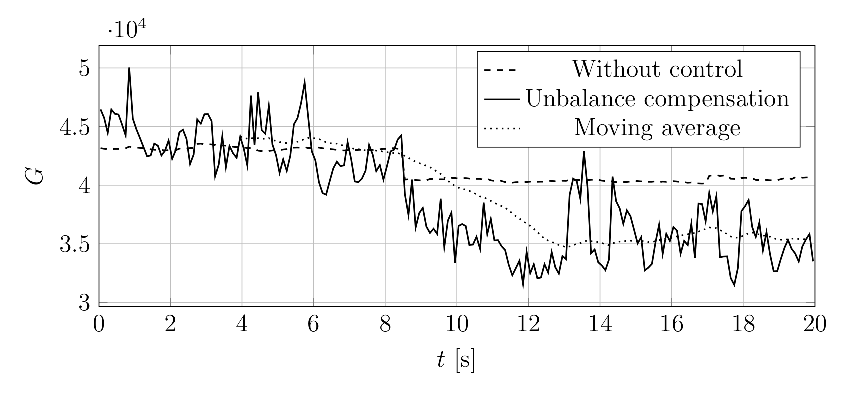
\includegraphics[width=0.95\textwidth]{Unblance_EPS_Pics/UnbalRedComp_JCP-figure4.eps}
            \caption{Unbalance reduction control system performance without battery and renewable source (zero energy balance operation). The performance reduction is clearly observable compared to the case when external power source is available (Figure \ref{fig:compare_asym_PV}), but as result the voltage unbalance indicator $G$ reduced by the average value of 14.78\%.}
            \label{fig:compare_asym}
            \end{figure*}

            A slightly more challenging situation is investigated in Figure \ref{fig:compare_asym} where the controller had had to operate without photovoltaic source and batteries. This is called zero balance operation mode when the energy obtained from the network is reinjected in such a way that the unbalance indicators decrease. It can be seen that the performance of the controller is modest than that of Figure \ref{fig:compare_asym_PV}, but it is still acceptable.

      \subsubsection{Robustness analysis}\label{VUB:sec:Robustness}

            The robustness of the proposed control structure is an important qualitative property with respect to the time dependent loads present on the network. The robustness of the proposed controller had to be tested via simulation when different types of loads (inductive, capacitive, resistive) had been varied in step changes representing representing the on/off switching the different types of household appliances (motors, switching mode power supplies, electric heaters, etc.). In the experiment depicted in Figure \ref{fig:robustness}, a load change has been introduced to the network in every 15 seconds causing the voltage unbalance to jump to a different value (measured in the geometrical norm (\ref{equ:geom})). As it can be seen in the figure the controller successfully compensates the unbalance after each transient.

              \begin{figure*}[ht]
            \centering
            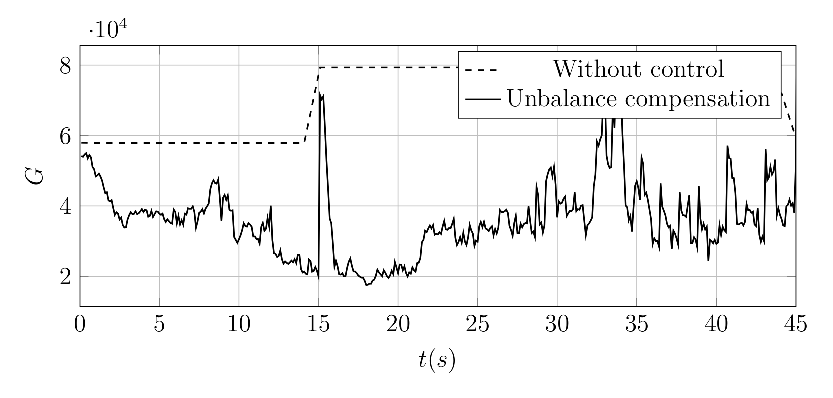
\includegraphics[width=0.95\textwidth]{Unblance_EPS_Pics/UnbalRedComp_JCP-figure5.eps}
            \caption{Robustness analysis with respect to step type changes in the network load (and voltage unbalance). The unbalance reduction controller successfully compensates the changes in the network voltage unbalance norm ($G$) value.}
            \label{fig:robustness}
            \end{figure*}

    \subsection{Environmental effect}\label{VUB:sec:Environment}

    The favorable effects of the proposed unbalance reduction control algorithm , i.e. increase power quality not only at the connection point but in the whole low voltage transformer area, which causes a reduction of the effective power loss and the reduction in the CO${}_2$ emission.

        \subsubsection{Power loss reduction on the network}\label{VUB:sec:Powerloss}

             Network loss reduction due to the unbalance reduction compensation control is investigated on Figure \ref{fig:compare_power} where the simulation experiment was carried out in the circumstance when the renewable source was not shut down (e.g. insufficient amount of sunlight) and additionally the battery was drained completely  \cite{Neukirchner2015}, \cite{neukirchner2015examination}.

            \begin{figure*}[ht]
            \centering
            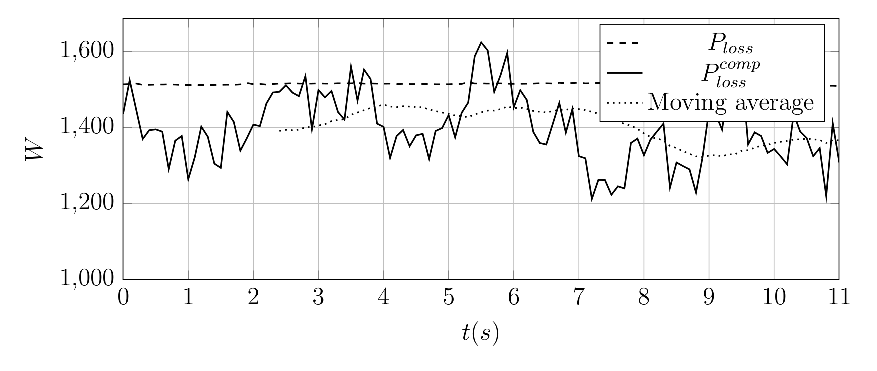
\includegraphics[width=0.95\textwidth]{Unblance_EPS_Pics/UnbalRedComp_JCP-figure6.eps}
            \caption{Compensation control's loss reduction during zero energy balance operation on the modeled network, where $P_{loss}$ indicates the effective power losses and $P^{comp}_{loss}$ effective power losses during control of the network. As result the network losses reduced by mean $6.5\%$.}
            \label{fig:compare_power}
            \end{figure*}

            The results show that despite of the negative cross effects of the intermediate voltage controller and the unbalance reduction controller it was possible to find the trade-off between the control goals of the different controllers (maintain zero energy balance for the inverter and decrease the unbalance on the network). The estimated loss reduction in the experimental setup is 6.5\%.

            \begin{figure*}[ht]
            \centering
            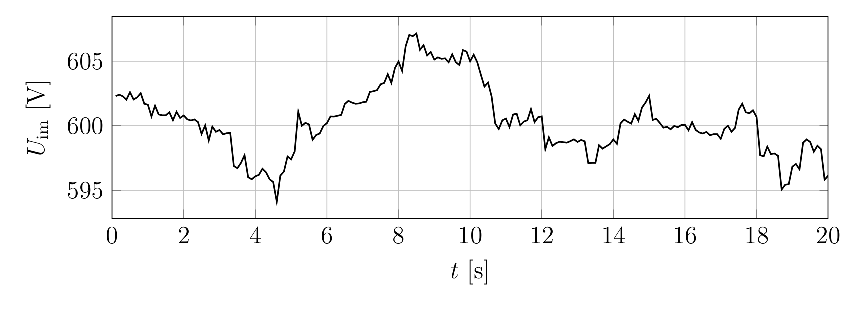
\includegraphics[width=0.95\textwidth]{Unblance_EPS_Pics/UnbalRedComp_JCP-figure7.eps}
%                  %\pgfplotsset{every tick label/.append style={font=\tiny},legend style={at={(1,1)},anchor=north east}}
%                 \pgfplotsset{every tick label/.append style={font=\normalsize}}
%                 \begin{tikzpicture}
%                 \begin{axis}[
%                     width=\textwidth,
%                     height=5cm,
%                     xlabel = {$t$~[s]},
%                     ylabel = {$U_{\textnormal{im}}$~[V]},
%                     grid=major,
%                     xmin=0,
%                     xmax=20,
%                     %ymin=0,
%                     ]
%                     \addplot[thick] table {netw_plot/U_inter.dat};
%                     %\legend{\scriptsize$U_{intermediate}$}
%                     \end{axis}
%                  \end{tikzpicture}
                 \caption{Intermediate puffer capacitance's voltage within boundaries ($600\pm10$\,V), during zero energy balance operation mode of the voltage unbalance compensation controller. $U_{\textnormal{im}}$ indicates intermediate the capacitance's voltage.}
                 \label{fig:u_inter}
                \end{figure*}

%        \subsubsection{Malfunction rejection}
%
%            asd

        \subsubsection[CO2 footprint]{CO$_2$ footprint}\label{VUB:sec:CO2}

            The fact that this controller enables the reactive power reduction has a favourable consequence, i.e. the power loss or equivalently CO$_2$ emission and the carbon footprint can also be decreased. The estimated environmental effects of voltage asymmetry compensation can be calculated. Let us assume 3000\,kWh for the yearly electric energy consumption an average household and $9.173\%$ for the loss of the distribution network \cite{MVM2013}. With the controller the losses on the simulated network are reduced by 6.5\%. The calculation follows (\ref{eqn:co_emission})

            \begin{equation}
                \label{eqn:co_emission}
                \begin{array}{rcl}
                 P_{loss}&=&3000\,\textnormal{kWh}\cdot9.173\%\\
                P^{comp}_{loss}&=&3000\,\textnormal{kWh}\cdot(9.173\cdot0.93)\%\\
                 \Delta P_{loss}&=&P_{loss}-P^{comp}_{loss}\\
                 \end{array}
                \end{equation}

            where $P_{loss}$ is the assumed network loss per household and $P^{comp}_{loss}$ is s the assumed network loss with unbalance compensation control and $\Delta P_{loss}$ is the saved energy. According to (\ref{eqn:co_emission}), unbalance compensation results in an energy savings of 19.26 kWh. Taking into account the proportion of power currently generated by fossil fuels (coal 17.3\%, gas 38.3\% at 2013 \cite{MVM2013}, \cite{gorbe2012reduction}) and the rate of $\textnormal{CO}_2$ emission during electric energy production (1,000\,g/kWh from coal and 430\,g/kWh from gas), it can be concluded that voltage unbalance compensation could reduce $\textnormal{CO}_2$ emissions by 6504.9\,g a year in 2013 in an average household. Note that this result reflect only the proof of concept, due the neglected power losses of the inverter and the artificial load of the network. 
						
						%654.8+107.6 
						% (coal 17.3\%, gas 38.3\% at 2013 \cite{MVM2013}, whilst 3.4\% and 1.3\% in 2015 \cite{gorbe2012reduction}) and the rate of $\textnormal{CO}_2$ emission during electric energy production (1,000\,g/kWh from coal and 430\,g/kWh from gas), it can be concluded that voltage unbalance compensation could reduce $\textnormal{CO}_2$ emissions by 6504.9\,g a year in 2013 and 762.4\,g in 2015, in an average household.

\section{Conclusion}\label{VUB:sec:Conclusion}

    Currently used measures of voltage unbalance (see section \ref{BASICUNB:sec:DefinitionsofUNB}) has been extended in this work with a new norm candidate, namely a geometrical norm, where the magnitude of voltage unbalance are evaluatad by the symmetrical difference of the voltge phasor triangles. It is more demanding from the computational point, of view but has an interesting feature namely it checks electrical asymmetry, i.e. the norm of a $\pm120$ degree  rotated version of the ideal three-phase phasor is zero in the geometrical sense.\\
    This way, the defined norm is applied as a cost function in the asymmetry reducing controller structure utilizing an asynchronous parallel pattern search (APPS) algorithm also presented in the thesis. Simulations, performed in Matlab/Simulink environment show that the geometrical based indicator can serve as a basis of further research. The suggested controller structure enables the residential users owning a grid synchronized domestic power (renewable) plant to reduce voltage unbalance measurable at the connection point. The fundamental element of the system is a modified three phase inverter that is capable of the asymmetric current injection of any current waveforms to the network, via decoupled bi-diectional DC-DC converters. The optimization based control algorithm injects the available energy (as current waveform) in such a way, that the voltage unbalance decreases. This is an optimization problem which is constrained by the available renewable energy supplied by the power plant.\\
    The control structure has been tested on a low voltage network model in a dynamical simulation environment consisting of the models of the electrical grid, a domestic power plant, an asymmetrical inverter circuit, and different types of loads. Different simulation experiments has been run for each norm and for both the power constrained and unconstrained case. The preliminary results show that this structure can serve as a residential level voltage quality improvement method for the three phase low voltage network also indirectly reduces the CO${}_2$ emission due facilitating more effective energy usage.

%\section{Voltage unbalance compensation with optimization based control algorithm and asymmetrical inverter structure}
%
%    Based on the proposed measures of voltage unbalance it is possible to formulate some power quality related aims, or demands for the domestic size generator units as follows.
%
%    \subsection{Problem statement}
%
%    The voltage and current unbalance presents in the three phase low voltage transformer area causes additional power loss inside the medium voltage/low voltage transformer and in the transportation line wires too. It also has undesired effects in certain three phase loads, mainly rotating machines where it causes torque reduction and pulsating torque effect. Large scale unbalance can activate automatic protection functions of electricity dispatch system causes power outage. This is unpleasant for the customers and adds maintenance cost to the service provider. These negative effects lower the electric power quality and rises the cost of electrical energy and rises the carbon footprint of our everyday life. Our aim to develop a three phase instrumentation, which can compensate these undesirable effects, lower or eliminate the voltage and current unbalance to lower the power losses and the CO${}_2$ emission and increase power quality not only at the connection point but in the whole low voltage transformer area. \emph{It is important to note, that this power quality improvement can be achieved without any significant added cost.} The aim is to integrate this function into an existing three phase photovoltaic inverter device connected to the low voltage grid, and the created complex energetic system is able to inject the renewable energy to the transportation network, can store the electrical energy from stochastic renewable sources in electrical vehicle batteries or feed the grid from the charged batteries in energy deficit and high demand simultaneous situations. Our new added value the integrated control algorithm which can highly lower or eliminate the observed unbalance of the network.
%
%    \subsection{Control problem}
%
%    The above problem statement partially specifies the solution space together with the solution method. The system of interest is the power grid with all the stochastic and nonlinear phenomena present in it. The input to the system is the current signals (one current in the single phase case and three in the three phase setup), which are naturally constrained by the available energy of the household - stored in a battery pack or momentarily generated by the wind or solar generator unit. The response of the system can be either the current or the voltage measured at the connection point of the inverter unit, however, the general legal regulations only allow voltage measurement for consumers. The difficulty of the control problem comes from the fact, that there are no mathematically tractable models of the network can be generated because of its unpredictable and nonlinear features. This means, that only black-box methods can be applied for this system.
%
%    For the control aim it is a natural choice to minimize the actual voltage unbalance of the low voltage local transformer area measured (or calculated) at the connection point of the inverter. Several optimization based methods are available for such kind of optimal control problems, e.g.  \cite{gorbe2012reduction} where the only bottleneck is the computational efficiency since the impemented controller has to run on the commercial inverter's hardware (digital singal processor unit).
%
%    \subsection{Asymmetrical inverter structure}
%
%    \textcolor{blue}{
%        The renewable energy injection is realized increasingly directly to the three phase low voltage grid in domestic size photovoltaic power plants too. This can reduce the voltage and current unbalance caused by the stochastic power production of wind and solar sources. More and more manufacturers produce three phase grid synchronized inverters from 5\,kW size. These equipments implement accurate symmetrical current feed with a standard three phase full bridge structure consists of six Isolated Gate Bipolar Transistors (IGBT). This is a cost effective standard structure suitable for symmetric harmonic current injection. It has limited capacities to inject not totally symmetric 3 phase current time functions, but Kirchhoff's current law permits only constant zero-sum current time functions injected with this structure. There are examples with this type of asymmetric current injections in the literature \cite{lee2010new}.}
%
%         %ide kellene a hivatkozás arra a cikkre, amit mutattál, ahol nem 120 fokosak a vektorok a fazor diagrammon, de az összegük 0
%    \textcolor{blue}{
%        This type of current injections has limited compensation capacity and this is not enough in  most asymmetric production and load cases. In our case we need more general, not specific asymmetric current waveforms, because the proposed control aim assumes the ability of injecting non zero-sum currents. This needs special inverter design structure. We need zero line connection for the differential current. One of the possible solution is to use 3 different full bridge single phase current inverters to supply each phase of low voltage transportation lines \cite{Patnaik2013topologies}. But in this case we need galvanic isolations of these single phase inverters in the output, or in the DC input size.}
%
%        %ide tegyük be hivatkozásnak: "Sushree Sangita Patnaik ., Anup Kumar Panda:Three-level H-bridge and three H-bridges-based three-phase four-wire shunt active power filter topologies for high voltage applications"
%    \textcolor{blue}{
%        This isolation can be reached  with using isolation transformers in the supply side. But we would like to use it a complex energetic system with specific inside true DC bus system feeded from Photovoltaic panel or batteries. We have to isolate  at least 2 full bridges with two way DC-DC converters. This can complicate the physical realization but easy to simulate with two controlled power source. Other possible easy to realize solution to isolate the full bridge outputs  connected to three phase lines with isolating transformers. It is recommended for operating and electric shock protection reasons too (Figure \ref{fig:asymminvwithgalvanic transformer}).Our distant aim to compensate other operational type line failures, such zero current appearing. This isolation method doesn't allow to produce CD current components, thats why we are looking for other design. Possible elegant solution to supplement the standard three phase inverter design with a fourth half bridge for Zero line, building a specific four leg inverter design \cite{Ninad2014control}.}
%
%        %ide tegyük be hivatkozásnak: "Nayeem Ahmed Ninad ., Luiz Lopes:Per-phase vector control strategy for a four-leg voltage source inverter operating with highly unbalanced loads in stand-alone hybrid systems"
%    \textcolor{blue}{
%        Only drawback of this solution is the complex difficult control method of the half bridges, to keep the current sum in zero values in each moment, and to provide the correct current paths inside the inverter. This structure has the lowest production cost, but in the phase of proofing the asymmetry compensation we chose the DC-DC isolated  full bridge design for simulation purpose because of the simple control during simulation.}
%    \textcolor{blue}{
%        As a further generalization step, the injection of no harmonic current shapes will be necessary in order to decrease the extant Total Harmonic Distortion (THD) of the network. These expectations yield an inverter with new structure suitable for arbitrary current injections without limitations. The design lends similar elements like in \cite{gorbe2012reduction} by means of battery charge, renewable power point tracking, intermediate voltage, and IGBT bridge control, but in this case the problem requires a three phase solution for the voltage unbalance reduction. The applied structure based on a full bridge IGBT structure used in single phase current injection. Three different IGBT full bridge were connected at the output point, thus our structure has three phase and neutral connection too, to carry out any current form. The disadvantage of this structure is that it needs 12 IGBTs in the output stage as opposed to the 6 IGBTs needed for a classical full bridge structure and needs three galvanically isolated direct current (DC) voltage source for feeding.}
%    \textcolor{blue}{The other standard elements, that the inverter design consists:}
%
%
%
%        \begin{itemize}
%            \item\textcolor{blue}{ Standard maximum power point tracking (MPPT) input stage, to inject the maximum available power from the renewable source to the intermediate voltage capacitor with a simple controlled boost converter}
%            \item\textcolor{blue}{ A half bridge current controller to charge or deploy the battery pack connected to the complex energetic system for energy storage and energy unbalance compensation}
%            \item\textcolor{blue}{ Intermediate voltage controller}
%            \item\textcolor{blue}{ Universal three phase output stage with 3 single phase full bridge IGBT current injector and 2 high current DC-DC converter}
%        \end{itemize}
%    \textcolor{blue}{
%        This is suitable to inject any necessary current shape to the low voltage three phase grid connection even DC currents too. Later a power loss and production cost analysis will be necessary if the built structure will be suitable for asymmetric compensation of low voltage transformer area.}
%
%        %\begin{figure*}[ht]
%%            \centering
%%            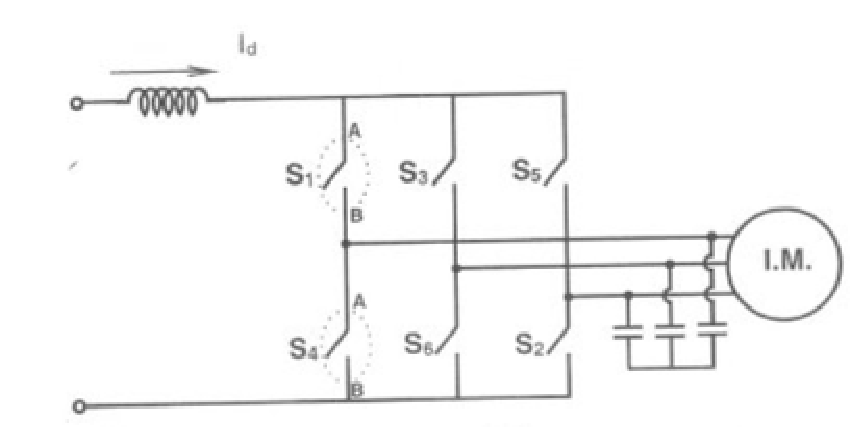
\includegraphics[width=0.95\textwidth]{standard_inverter.eps}
%%            \caption{\textcolor{blue}{Standard symmetrical current inverter design, implies 6 IGBT current injector with serial inductance. }}
%%        \label{fig: symminv}
%%        \end{figure*}
%
%        %\begin{figure*}[ht]
%%            \centering
%%            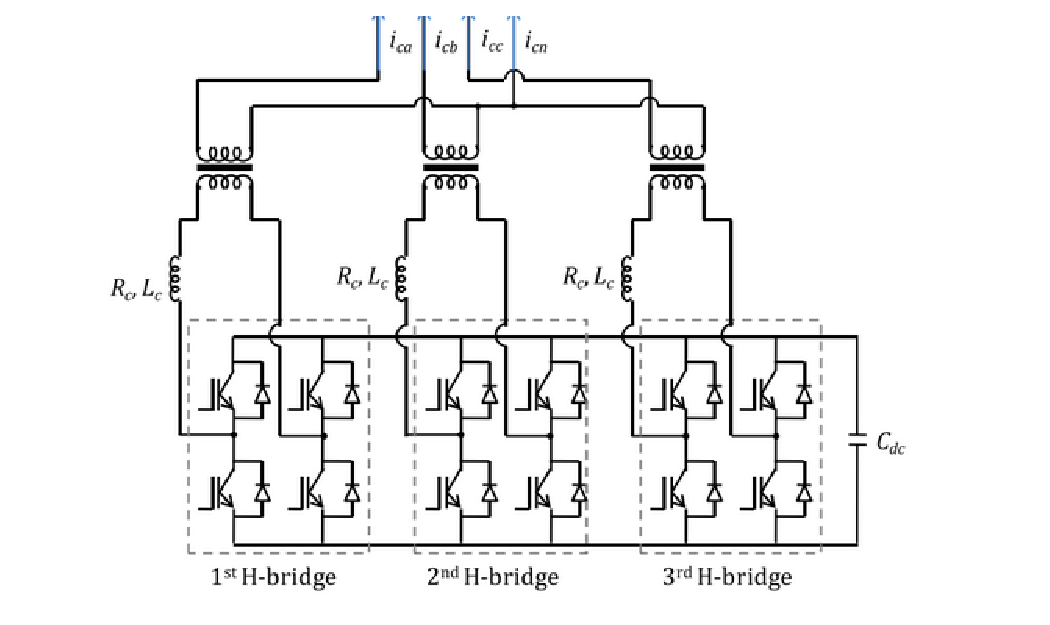
\includegraphics[width=0.95\textwidth]{isolated_inverter.eps}
%%            \caption{\textcolor{blue}{Asymmetrical inverter design with three separated H-bridges.}}
%%        \label{fig: asymminvwithDCgalvanic transformer}
%%        \end{figure*}
%
%\begin{figure}[h]
%          \begin{center}
%                \begin{circuitikz}[scale=.5, european] %% => Itt ne állíts a skálát, inkább a figure-nél!%%
%                %\draw[help lines] (0,0) grid (16,40);
%
%                \draw%[color=magenta]
%                    %% híd
%                    (0,0) to[C=$C_{intermediate}$] (0,38)
%                    (0,0) to[short] (10,0)
%                    (6,0) node[nigbt, anchor=E](nigbt33){}
%                    (nigbt33.E) node[circ]{}
%
%                    (10,8) node[nigbt, anchor=E,xscale=-1](nigbt32){}
%
%                    (6,8) node[nigbt, anchor=E](nigbt31){}
%                    (nigbt33.C) to[short] (nigbt31.E)
%
%                    (10,0) node[nigbt, anchor=E, xscale=-1](nigbt34){}
%                    (nigbt34.C) to[short] (nigbt32.E)
%
%                    (nigbt32.C) to[short] (10,12)
%                    (nigbt31.C) to[short,-*] (6,12)
%                    (4,12) to[short] (10,12)
%                    (4,12) to[short,-*] (4,38)
%
%
%                    %%trafó
%                    (7,6) node[transformer,rotate=90,transform shape,american](T3){}
%                    (T3.B1) to[short,-*] (6,7.05)
%                    (T3.B2) to[short,-*] (10,7.05)
%                    (T3.A1) to[short] (7,4)
%                    (7,4) to[short,-o] (13,4) node[anchor=west] {$N$}
%                    (T3.A2) to[short,-o] (13,4.95) node[anchor=west] {$T$}
%                    ;
%
%                    \draw%[color=blue]
%                    %% híd
%                    (3,13) to[short,*-] (10,13)
%                    (6,13) node[nigbt, anchor=E](nigbt23){}
%                    (nigbt23.E) node[circ]{}
%
%                    (10,21) node[nigbt, anchor=E,xscale=-1](nigbt22){}
%
%                    (6,21) node[nigbt, anchor=E](nigbt21){}
%                    (nigbt23.C) to[short] (nigbt21.E)
%
%                    (10,13) node[nigbt, anchor=E, xscale=-1](nigbt24){}
%                    (nigbt24.C) to[short] (nigbt22.E)
%
%                    (nigbt22.C) to[short] (10,25)
%                    (nigbt21.C) to[short,-*] (6,25)
%                    (4,25) to[short,*-] (10,25)
%
%
%
%
%                    %%trafó
%                    (7,19) node[transformer,rotate=90,transform shape,american](T2){}
%                    (T2.B1) to[short,-*] (6,20.05)
%                    (T2.B2) to[short,-*] (10,20.05)
%                    (T2.A1) to[short] (7,17)
%                    (7,17) to[short,-*] (12,17)
%                    (T2.A2) to[short,-o] (13,17.95) node[anchor=west] {$S$}
%                    ;
%
%                    \draw%[color=cyan]
%                    %% híd
%                    (3,26) to[short] (10,26)
%                    (3,26) to[short,-*] (3,0)
%
%                    (6,26) node[nigbt, anchor=E](nigbt13){}
%                    (nigbt13.E) node[circ]{}
%
%                    (10,34) node[nigbt, anchor=E,xscale=-1](nigbt12){}
%
%                    (6,34) node[nigbt, anchor=E](nigbt11){}
%                    (nigbt13.C) to[short] (nigbt11.E)
%
%                    (10,26) node[nigbt, anchor=E, xscale=-1](nigbt14){}
%                    (nigbt14.C) to[short] (nigbt12.E)
%
%                    (nigbt12.C) to[short] (10,38)
%                    (nigbt11.C) to[short,-*] (6,38)
%                    (0,38) to[short] (10,38)
%
%
%                    %%trafó
%                    (7,32) node[transformer,rotate=90,transform shape,american](T1){}
%                    (T1.B1) to[short,-*] (6,33.05)
%                    (T1.B2) to[short,-*] (10,33.05)
%                    (T1.A1) to[short] (7,30)
%                    (7,30) to[short] (12,30)
%                    (12,30) to[short,-*] (12,4)
%                    (T1.A2) to[short,-o] (13,30.95) node[anchor=west] {$R$}
%                    ;
%                %%
%                \end{circuitikz}
%                \caption{\textcolor{blue}{Simplified asymmetrical inverter design employing three galvanically isolated H-bridges with transformers for DC-DC isolation substitution.}}
%                \label{fig: asymminvwithgalvanic transformer}
%          \end{center}
%    \end{figure}
%
%        %\begin{figure*}[ht]
%%            \centering
%%            \includegraphics[width=0.95\textwidth]{isolated_only_inverter.eps}
%%            \caption{\textcolor{blue}{Simplified asymmetrical inverter design employing three galvanically isolated H-bridges with transformers for DC-DC isolation substitution.}}
%%        \label{fig: asymminvwithgalvanic transformer}
%%        \end{figure*}
%
%
%        \begin{figure*}[ht]
%        \centering
%        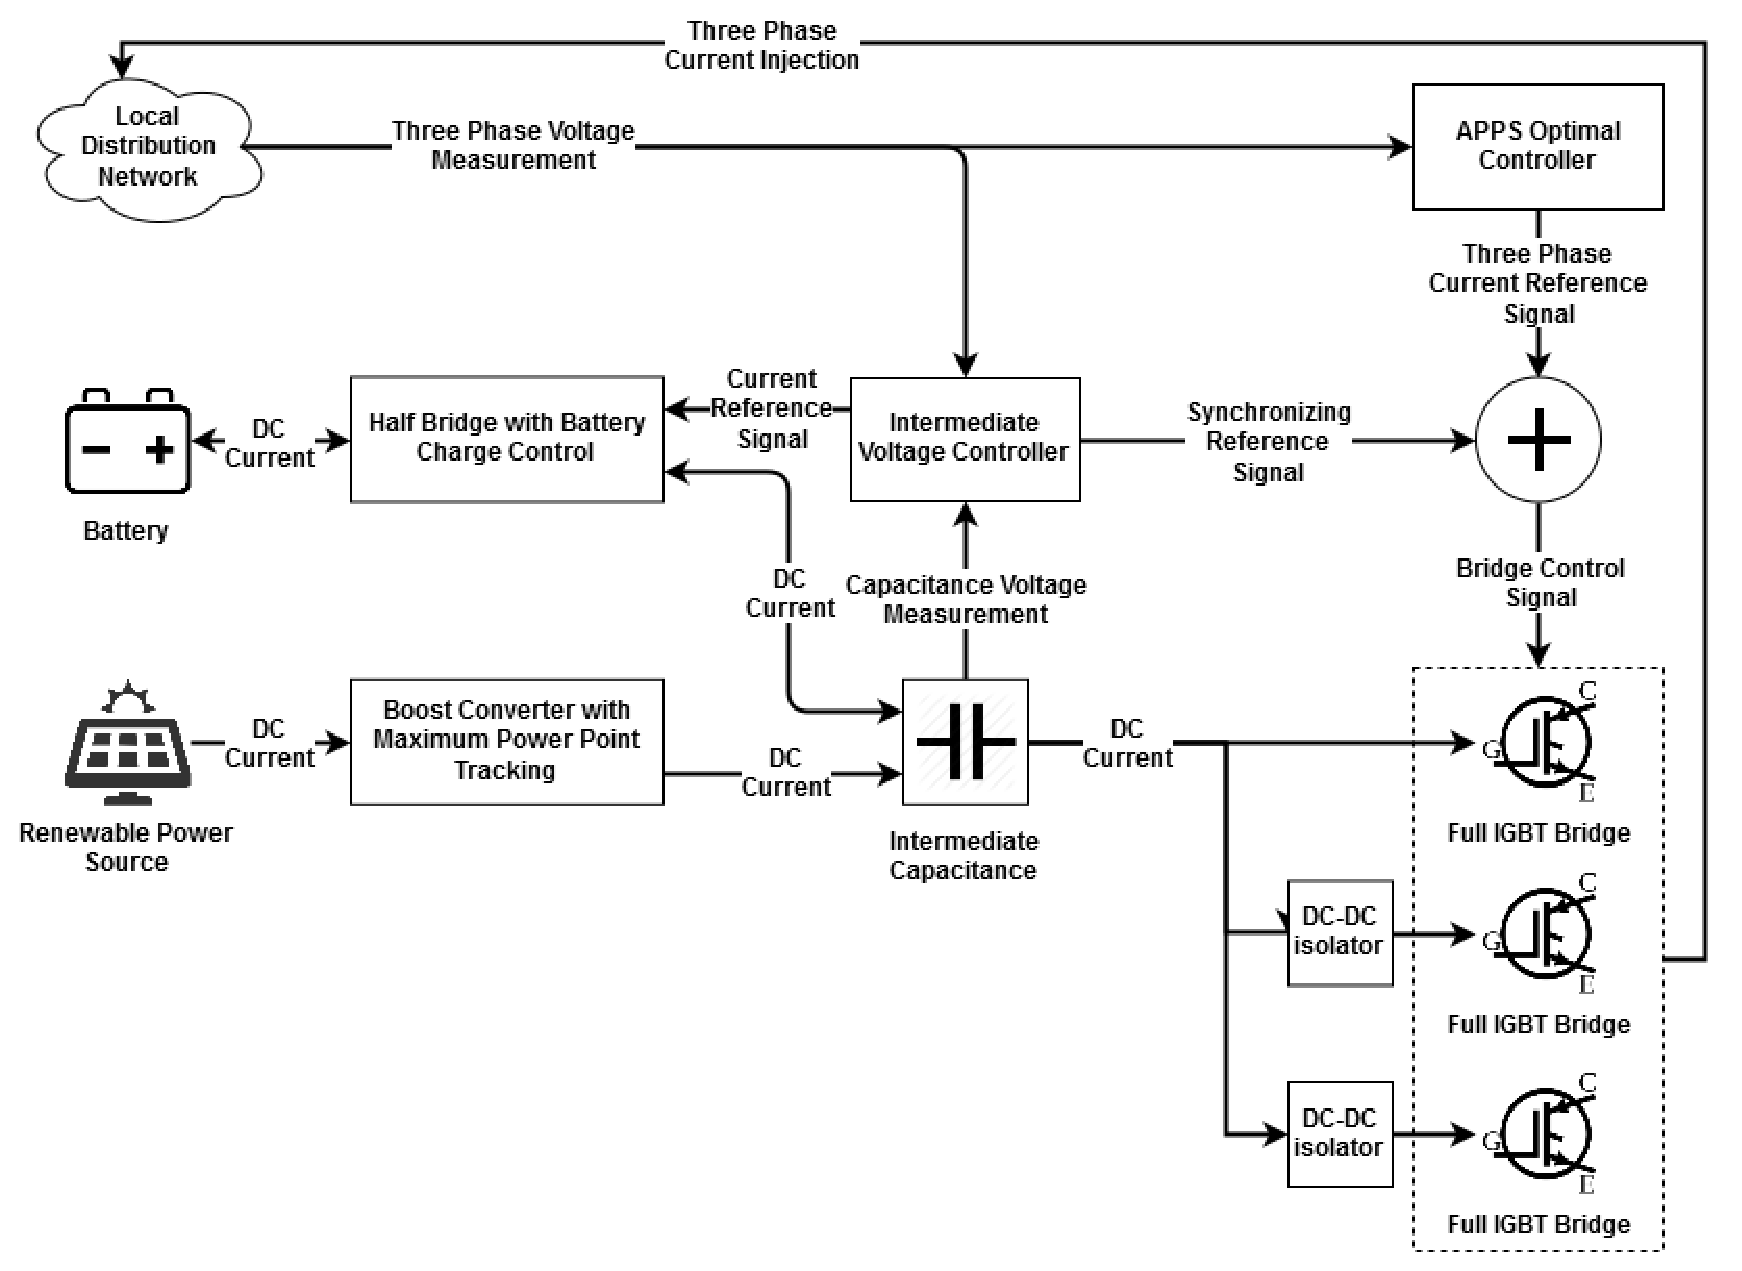
\includegraphics[width=0.95\textwidth]{Unblance_EPS_Pics/inverter.eps}
%        \caption{\textcolor{blue}{The asymmetrical inverter design, which applies three single phase full bridge IGBT current injector to create the injected asymmetrical current shapes for voltage unbalance compensation. }}
%        \label{fig:inv}
%        \end{figure*}
%
%    \textcolor{blue}{
%        Of course there is a possibility that there is no renewable power available for a longer period of time and the battery completely looses its charge. In this case the system should work merely with the power of the connection point but with  zero energy balance. This states to operate two controller with semi-opposite control goals. The optimization based controller requires current injection while the intermediate voltage controller (Figure \ref{fig:inv}) keeps the inverters energy balance. Although for this operation some of the control's performance should be sacrificed, unbalance compensation could be achieved even without external renewable power, and energy storage at a minimum power requirement.}
%        %\subsubsection{The necessity of switching the control off}
%%
%%                \textcolor{blue}{Inverter lea\'all\'it\'as\'anak sz\"uks\'egess\'ege.}
%
%%
%        The renewable energy injection is realized increasingly directly to the three phase low voltage grid in domestic size photovoltaic power plants too. This can reduce the voltage and current unbalance caused by the stochastic power production wind and solar sources. More and more manufacturers produce three phase grid synchronized inverters from 5\,kW size. These equipments implement symmetrical power feed with a standard three phase full bridge structure consists of six Isolated Gate Bipolar Transistors (IGBT). This is a cost effective standard structure suitable for symmetric harmonic current injection, but Kirchhoff's current law permits only constant zero-sum current time functions injected with this structure. The proposed control aim assumes the ability of injecting non constant zero-sum currents. As a further generalization step, the injection of no harmonic current shapes will be necessary in order to decrease the extant Total Harmonic Distortion (THD) of the network. These expectations yield an inverter with new structure suitable for arbitrary current injections without limitations. The design lends similar elements like in \cite{gorbe2012reduction} by means of battery charge, renewable power point tracking, intermediate voltage, and IGBT bridge control, but in this case the problem requires a three phase solution for the voltage unbalance reduction. The applied structure based on a full bridge IGBT structure used in single phase current injection. Three different IGBT full bridge were connected at the output point, thus our structure has three phase and neutral connection too, to carry out any current form. The disadvantage of this structure is that it needs 12 IGBTs in the output stage as opposed to the 6 IGBTs needed for a classical full bridge structure and needs three galvanically isolated direct current (DC) voltage source for feeding. \\
%        The other standard elements, that the inverter design consists:
%        \begin{itemize}
%            \item Standard maximum power point tracking (MPPT) input stage, to inject the maximum available power from the renewable source to the intermediate voltage capacitor with a simple controlled boost converter
%            \item A half bridge current controller to charge or deploy the battery pack connected to the complex energetic system for energy storage and energy unbalance compensation
%            \item Intermediate voltage controller
%            \item Universal three phase output stage with 3 single phase full bridge IGBT current injector and 2 high current DC-DC converter
%        \end{itemize}
%        This is suitable to inject any necessary current shape to the low voltage three phase grid connection even DC currents too. Later a power loss and production cost analysis will be necessary if the built structure will be suitable for asymmetric compensation of low voltage transformer area.
%
%        %\begin{figure*}[ht]
%%        \centering
%%        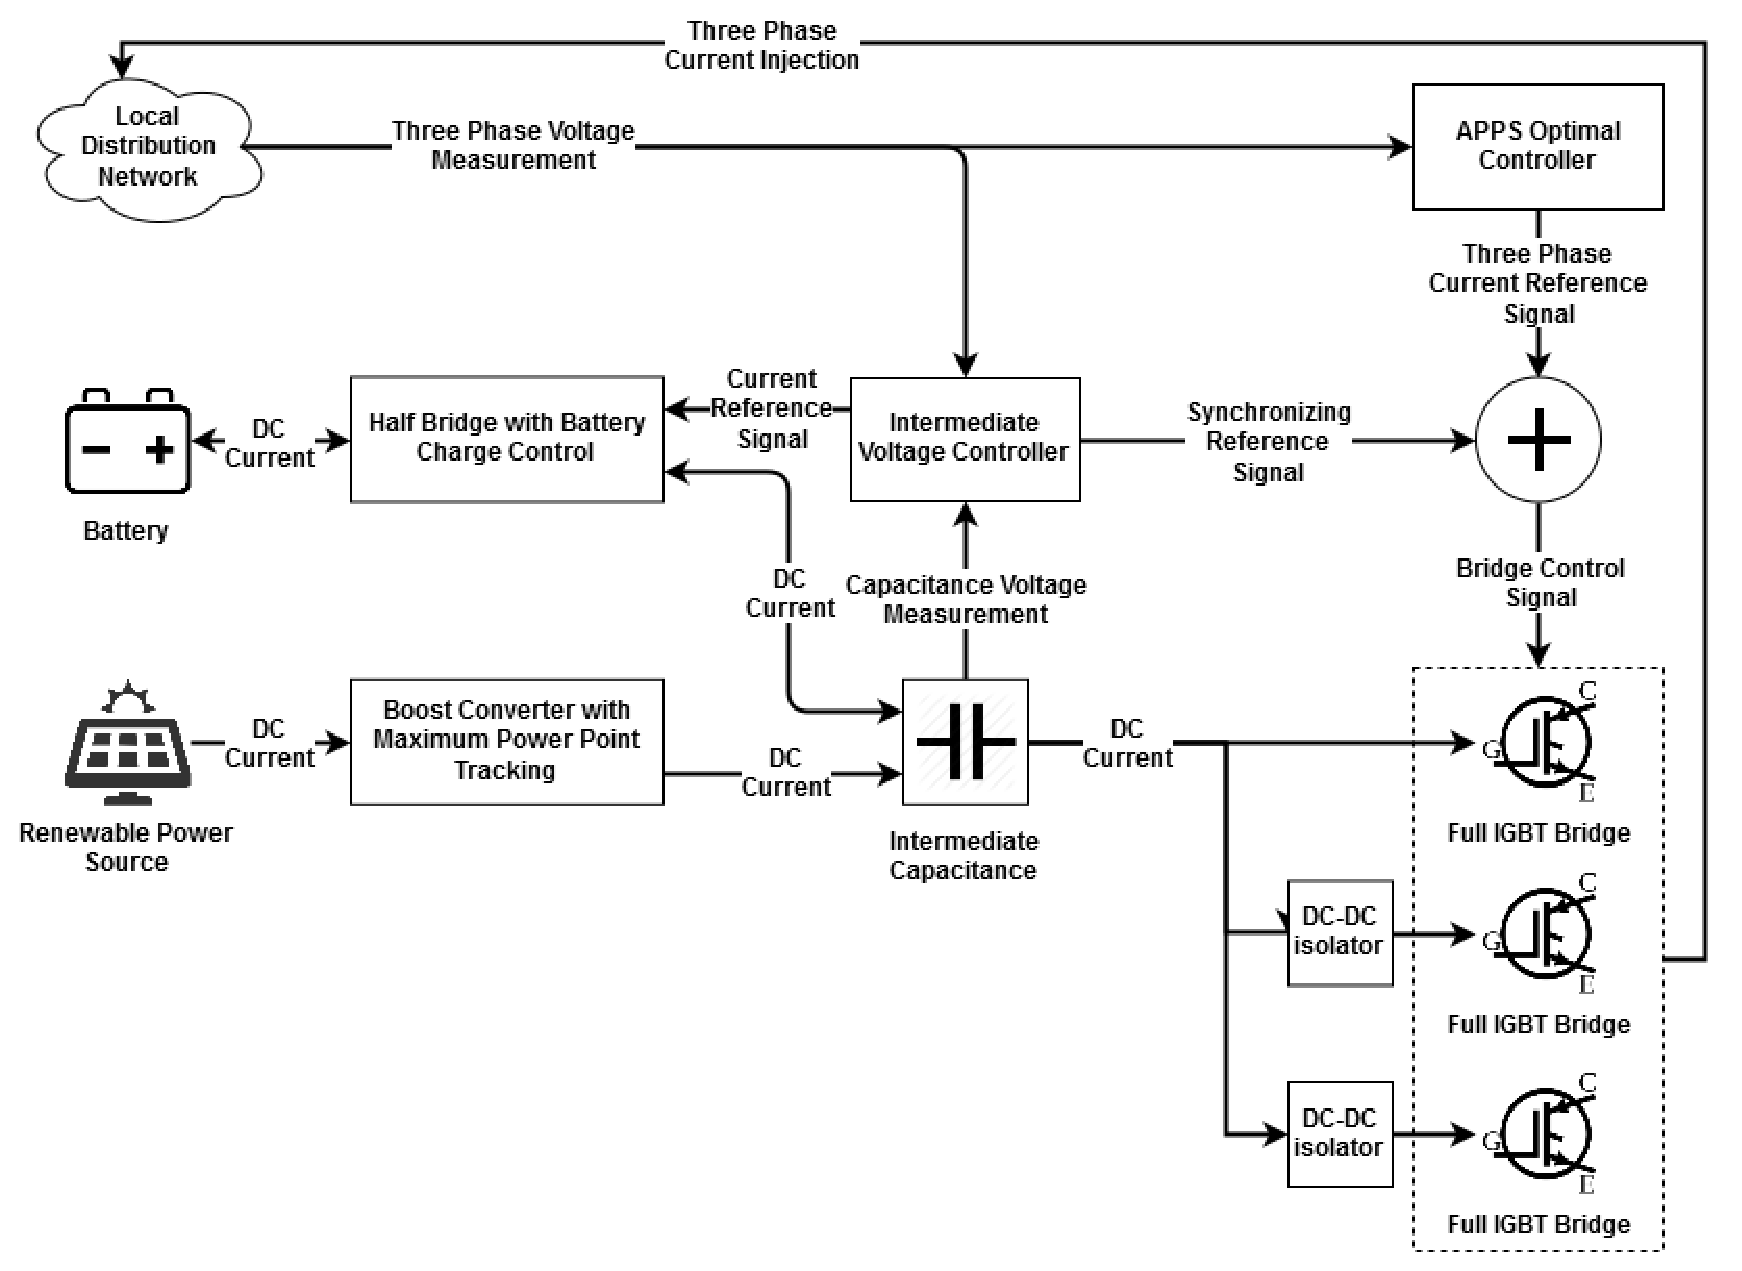
\includegraphics[width=0.95\textwidth]{Unblance_EPS_Pics/inverter.eps}
%%        \caption{The asymmetrical inverter design, which implies 3 single phase full bridge IGBT current injector to form the injected asymmetrical current shapes for voltage unbalance compensation. }
%%        \label{fig:inv}
%%        \end{figure*}
%%
%        Of course there is a possibility that there is no renewable power available for a longer period of time and the battery completely looses its charge. In this case the system should work merely with the power of the connection point but with  zero energy balance. This states to operate two controller with semi-opposite control goals. The optimization based controller requires current injection while the intermediate voltage controller (Figure \ref{fig:inv}) keeps the inverters energy balance. Although for this operation some of the control's performance should be sacrificed, unbalance compensation could be achieved even without external renewable power, and energy storage at a minimum power requirement.
%        %\subsubsection{The necessity of switching the control off}
%%
%%                \textcolor{blue}{Inverter lea\'all\'it\'as\'anak sz\"uks\'egess\'ege.}
%
%        \subsubsection{Measurements from a real unbalanced network}
%
%            The measurements took place at the Faculty's building, where a common 400\,V connection point was investigated as the behaviour of the network. The three phase 230\,V line-to-ground voltages has been transformed to 6\,V to be effectively measurable time domain with high performance NI-USB DAQ on 10\,ksample/s. Because of the limited computational capacity only a 10 second measurement was made in every hour.  The measurements then has been merged and smoothed to eliminate the inter-measurement transients.\\
%            Afterwards, the measurement data has been used as the output of a micro-grid segment of the Matlab/Simulink model, to test the controller and inverters structure's performance in quasi-realistic circumstances. The controllers performance on the simulated microgrid's network loss reduction can be observed on (Figure \ref{fig:compare_power}). The measurement output is connected to a modeled three phase load and network system, consisting of symmetrical loads and network segments between them. Further artificial load unbalance is not necessary since the network's unbalance is already present. This structure enables to show that any point the inverter is connected could serve as quality restoration such unbalance compensation at this case. Our future plan is to set up multiple devices on different connection points.
%
%
%
%    \subsection{Optimization based control algorithm}
%
%        \begin{figure*}[ht]
%        \centering
%        \includegraphics[width=0.95\textwidth]{Unblance_EPS_Pics/APPS_grey.eps}
%        \caption{\textcolor{blue}{The optimization algorithm implemented for current control. A one dimensional linear optimization step is being solved in each dimension of the six dimensional parameter space, iteratively.}}
%        \label{fig:APPS}
%        \end{figure*}
%
%        The problem is that, the exact mathematical relation is nonlinear because the nonlinear, and highly time variant loads of the network, we should use a control strategy to cope this nonlinear and time variant energy system. For this purpose we chose an asynchronous parallel pattern search method (APPS) which could be able to control our scenario.  We applied a variant of the gradient method that is a first-order optimization (minimization) algorithm for a multivariate function $f(x)$. The point $x(k)$ corresponding to the local minimum can be calculated from the negative gradient $\delta f(x)$, that gives the value and direction of the corresponding step in the parameter space. The next step is made in the direction of gradient with the proper sign. This sequence of steps, ideally, converges to local multivariate extreme value $x(k)$ of the function (\ref{eqn:contstruct1}).
%
%        \begin{equation}
%        \begin{array}{rcl}
%        \label{eqn:contstruct1}
%         x^{(k)}&=&x^{(k-1)}-t_k \nabla f(x^{(k-1)})\\
%         k&\in&\mathbb{N}\\
%         \end{array}
%        \end{equation}
%
%        The controlled electrical system is described by multivariate non-linear differential equations, the optimization of which is infeasible to derive using the differentiation of an error function. Therefore, the optimization methods based on direct differentiation are not applicable. In such cases, when high computational power is needed for performing long time-consuming simulations, the APPS method can utilized. The search pattern $p$ is based on the sampling of the error function (selected norm) on a "grid", and it corresponds to variables or subsets of variables in each point in the independent variable or parameter space easily. At the same time, the norm values at these points can be calculated independently if $\Delta k>0$, using (\ref{eqn:contstruct2}).
%        \begin{equation}
%        \label{eqn:contstruct2}
%        \begin{array}{rcl}
%         x^{(k+1)}&=&x^{(k)}+\Delta _kd_i \\
%         \mathrm{if}&&f(x^{(k)}+\Delta _kd_i) \leq f(x^{(k)})\\
%         k&\in&\mathbb{N}\\
%         \end{array}
%        \end{equation}
%
%        The parameter is  $x(k)\in R_n$, and the search pattern $p\in D={d_1,...d_n}$ is taken from a predefined finite set. In this case, the error function values should be calculated for each pattern $p$ in the set $D$. If the error function is not decreasing in any of the directions, then the step size should be reduced (e.g. by half). As the competing directions are different, if there is not enough computing power available for direction vector $p$, synchronization should not be maintained. In this case we are talking about the asynchronous case . In the case of our controller, an individual $p$ vector is defined for each output variable, and the optimization was performed in each direction asynchronously and shifted in time. Most likely, the error function has a single local minimum as a symmetric amplitude and phase values. Approaching the minimal value of norm, the controller uses adaptive increments that are proportional to the norm itself. Because of the complex interactions between the components of the controller, only one parameter is changed at a time, even if the values of the amplitude and phase components in specific time slot changes. The algorithm moves along the six axes of six separate time slots close to the local minimum of the error function.\\
%        Unlike other similar approaches, e.g. \cite{segui2007approach}, the explained optimal controller does not rely on a measured current signal but rather measuring and analysing the voltage unbalance via the proposed indicator and optimizes the voltage shape, the latter of which depends on the nonlinear distortion of the whole low-voltage transformer area and determines additional power losses. The controller's performance was compared to a non compensated network, and a network consisting synchronised symmetric power intake from a regular inverter.\\
%        In each iteration only one physical value is changing on the six dimensional parameter field, which consists of the three amplitude and three phase values. If the change effects with cost function reduction (the reference norm's normalised value), the controller holds the new value of amplitude or phase for the controlled current sources. The advantage of this controller structure that is not necessary to know the controlled value's behaviour well, like we could not determine the number and type of the other loads on the network \cite{Neukirchner2015}. There are however two disadvantages. First is the low speed of control, due to the several necessary iterations (depending on the circumstances) to find the optimal directions in the parameter space, and the serial nature of interventions and norm calculations. The second comes from the method itself since the controller may stuck in local minima.
%
%    %\subsubsection{Higher level control structure}
%%
%%            \begin{itemize}
%%            \item \textcolor{blue}{Norm\'al \'es z\'er\'o energimam\'erleg \"uzemm\'odok.}
%%            \item \textcolor{blue}{\"Uzemm\'od v\'altasok.}
%%            \end{itemize}
%
%\subsection{Discussion}
%    \subsubsection{Dynamical simulation based experiments}
%    In order to be able to investigate the proposed optimization based unbalance reduction control structure with the three phase inverter on a low voltage local grid, all the elements of this complex electrical system (including the photovoltaic source, the inverter, the battery and the nonlinear local grid with different types of loads) has been modeled in Matlab/Simulink environment. The primary aim of the simulation based experiments were to serve as a proof of concept for the proposed complex control structure.
%    \subsubsection{Performance analysis}
%    The aim of performance analysis is twofold. First of all, the proposed voltage unbalance indicator has to be investigated in the control structure as the cost function of the optimization based controller, and on the other hand, the control structure itself has to be exposed against engineering expectations.
%
%%     The first experiment is depicted in Figure \ref{fig:compare_asym_VEC}, where the vectorial based voltage unbalance indicator was used as the cost function of the optimization algorithm. The results are far not promising since the value of norm $N$ of the network starts to oscillate when the unbalance reduction controller is active. The cause of this behaviour is \textcolor{red}{WHAT?}
%%
%%             % V ==========================
%%            \begin{figure*}[h]
%%             \centering
%%                  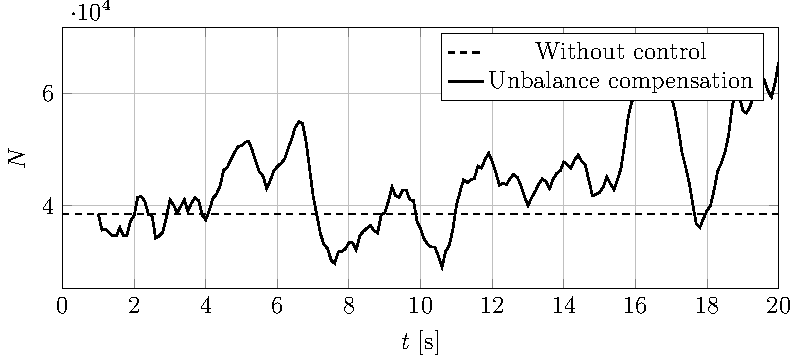
\includegraphics{UnbalRedComp_JCP-figure2.pdf}
%% %                 \pgfplotsset{every tick label/.append style={font=\normalsize}}
%% %                 \begin{tikzpicture}
%% %                 \begin{axis}[
%% %                     width=\textwidth,
%% %                     height=6cm,
%% %                     xlabel = {$t$~[s]},
%% %                     ylabel = {$N$},
%% %                     grid=major,
%% %                     xmin=0,
%% %                     xmax=20,
%% %                     %ymax=8000,
%% %                     %ymin=200,
%% %                     ]
%% %                     \addplot [dashed, thick] coordinates {(0,38520) (20,38520)};
%% %                     \addplot[thick] table {VEC_Measurements/VEC_orig.dat};
%% %                     \legend{Without control, Unbalance compensation}
%% %                     \end{axis}
%% %                  \end{tikzpicture}
%%                  \caption{Compensation control's voltage unbalance reduction, where $N$ indicates the calculation with the vectorial indicator value. The controller starts at $t=0.1s$ and starts oscillating towards unbalance.}
%%                  \label{fig:compare_asym_VEC}
%%                 \end{figure*}
%
%                The results of the first experiment can be seen in Figure \ref{fig:compare_asym_PV} where the geometrical norm \ref{equ:geom} has been used as the voltage unbalance indicator and the cost function for the optimizer.  The dashed line represents the examined low voltage local network's unbalance norm ($G$) without the proposed controller implemented in the inverter unit of the domestic powerplant while the solid line represents the compensated network'snorm value. The performance of the controller with this norm is apparent, it was able to decrease the network voltage unbalance by approximately 85 \%. In this experimental setup the controller has enough input energy due to the batteries and the available solar power.
%
%            % G ========================== +PV
%            \begin{figure*}[ht]
%            \centering
%            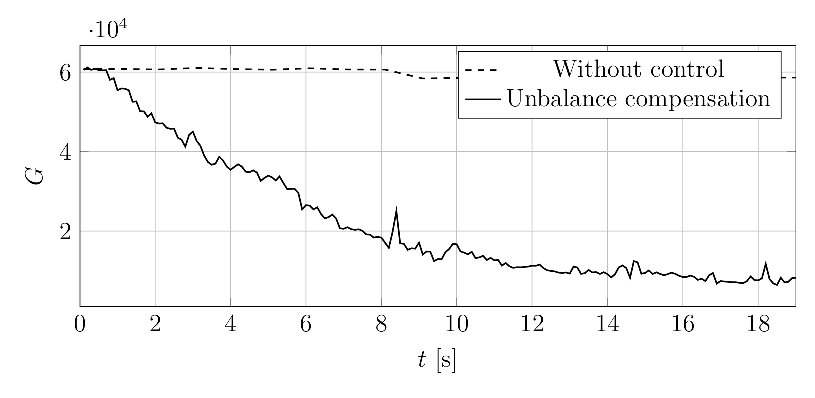
\includegraphics[width=0.95\textwidth]{Unblance_EPS_Pics/UnbalRedComp_JCP-figure3.eps}
%%                 %\pgfplotsset{every tick label/.append style={font=\tiny},legend style={at={(1,1)},anchor=north east}}
%%                 \pgfplotsset{every tick label/.append style={font=\normalsize}}
%%                 \begin{tikzpicture}
%%                 \begin{axis}[
%%                     width=\textwidth,
%%                     height=6cm,
%%                     xlabel = {$t$~[s]},
%%                     ylabel = {$G$},
%%                     grid=major,
%%                     xmin=0,
%%                     xmax=19,
%%                     %ymax=900,
%%                     %ymin=200,
%%                     ]
%%                     \addplot[dashed,thick] table {withPV/GEO_nocont_orig.dat};
%%                     \addplot[thick] table {withPV/GEO_orig.dat};
%%                     \legend{Without control, Unbalance compensation}
%%                     \end{axis}
%%                  \end{tikzpicture}
%                 \caption{Unbalance reduction control system performance with half charged battery and photovoltaic power source available. The underlying unbalance norm is the geometrical one ($G$) in this experiment. After starting the controller at $t=0.1s$ the unbalance measure $G$ of the network significantly decrease.}
%                 \label{fig:compare_asym_PV}
%                \end{figure*}
%
%                % G ========================== -PV
%            \begin{figure*}[ht]
%            \centering
%            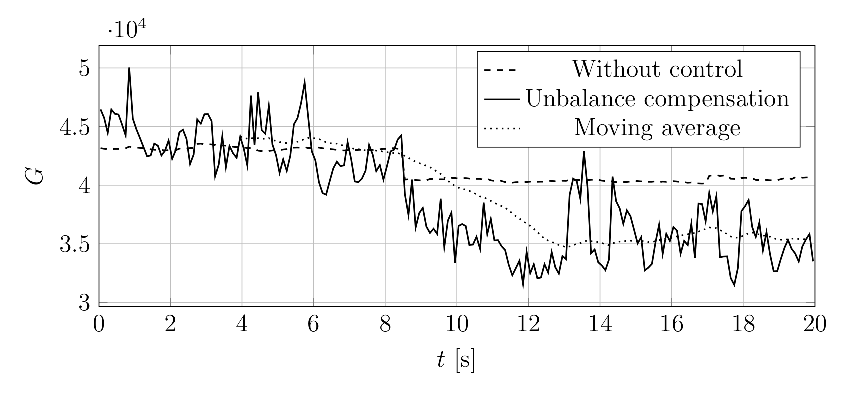
\includegraphics[width=0.95\textwidth]{Unblance_EPS_Pics/UnbalRedComp_JCP-figure4.eps}
%%                  %\pgfplotsset{every tick label/.append style={font=\tiny},legend style={at={(1,1)},anchor=north east}}
%%                 \pgfplotsset{every tick label/.append style={font=\normalsize}}
%%                 \begin{tikzpicture}
%%                 \begin{axis}[
%%                     width=\textwidth,
%%                     height=6cm,
%%                     xlabel = {$t$~[s]},
%%                     ylabel = {$G$},
%%                     grid=major,
%%                     xmin=0,
%%                     xmax=20,
%%                     %ymax=600,
%%                     %ymin=200,
%%                     ]
%%                     \addplot[dashed,thick] table {netw_plot_nocont/GEO_nocont_orig.dat};
%%                     \addplot[thick] table {netw_plot/GEO_orig.dat};
%%                     \addplot[dotted,thick] table {netw_plot/GEO_orig_mean.dat};
%%                     \legend{Without control, Unbalance compensation, Moving average}
%%                     \end{axis}
%%                  \end{tikzpicture}
%                 \caption{Unbalance reduction control system performance without battery and renewable source (zero energy balance operation). The performance reduction is clearly observable compared to the case when external power source is available (Figure \ref{fig:compare_asym_PV}), but as result the voltage unbalance indicator $G$ reduced by the average value of 14.78\%.}
%                 \label{fig:compare_asym}
%                \end{figure*}
%
%            A slightly more challangeing situation is investigated in Figure \ref{fig:compare_asym} where the controller had had to operate without photovoltaic source and batteries. This is called zero balance operation mode when the energy obtained from the network is reinjected in such a way that the unbalance indicators decrease. It can be seen that the performance of the controller is modest than that of Figure \ref{fig:compare_asym_PV}, but it is still acceptable.
%
%      \paragraph{Robustness analysis}
%
%            %\textcolor{magenta}{MACI}\\
%            %\textcolor{blue}{Robosztuss\'agi vizsg\'alat mind norm\'al mind zero balance esetre.}
%            The robustness of the proposed control structure is an important qualitative property with respect to the time dependent loads present on the network. The robustness of the proposed controller had to be tested via simulation when different types of loads (inductive, capacitive, resistive) had been varied in step changes representing represnting the on/off switching the different types of household appliances (motors, switching mode power supplies, electric heaters, stc.). In the experiment depicted in Figure \ref{fig:robustness}, a load change has been introduced to the network in every 15 seconds causing the voltage unbalance to jump to a different value (measured in the geometrical norm (\ref{equ:geom})). As it can be seen in the figure the controller successfully compensates the unbalance after each transient.
%
%              \begin{figure*}[ht]
%            \centering
%            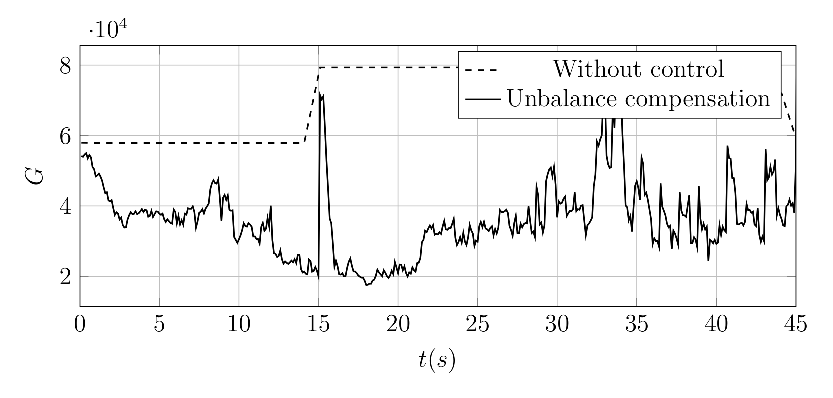
\includegraphics[width=0.95\textwidth]{Unblance_EPS_Pics/UnbalRedComp_JCP-figure5.eps}
%%             %\pgfplotsset{every tick label/.append style={font=\tiny},legend style={at={(1,1)},anchor=north east}}
%%             \pgfplotsset{every tick label/.append style={font=\normalsize}}
%%             \begin{tikzpicture}
%%             \begin{axis}[
%%             width=\textwidth,
%%             height=6cm,
%%             xlabel = {${t(s)}$},
%%             ylabel = {${G}$},
%%             grid=major,
%%             xmin=0,
%%             xmax=45,
%%             %ymax=140,
%%             ]
%%             \addplot[thick, dashed] table {robustness_nocont/GEO_nocont_orig.dat};
%%             \addplot[thick] table {robustness_regular/GEO_orig.dat};
%%             \legend{Without control, Unbalance compensation}
%%             \end{axis}
%%             \end{tikzpicture}
%            \caption{Robustness analysis with respect to step type changes in the network load (and voltage unbalance). The unbalance reduction controller successfully compensates the changes in the network voltage unbalance norm ($G$) value.}
%            \label{fig:robustness}
%            \end{figure*}
%
%
%
%    \subsubsection{Environmental effect}
%            favorable effects of the proposed unbalance reduction control algorithm , i.e. increase power quality not only at the connection point but in the whole low voltage transformer area, which causes a reduction of the effective power loss and the reduction in the CO${}_2$ emission.
%
%        \paragraph{Power loss reduction on the network}
%
%             Network loss reduction due to the unbalance reduction compensation control is investigated on Figure \ref{fig:compare_power} where the simulation experiment was carried out in the circumstance when the renewable source was not shut down (e.g. insufficient amount of sunlight) and additionally the battery was drained completely  \cite{Neukirchner2015}, \cite{neukirchner2015examination}.
%            \begin{figure*}[ht]
%            \centering
%            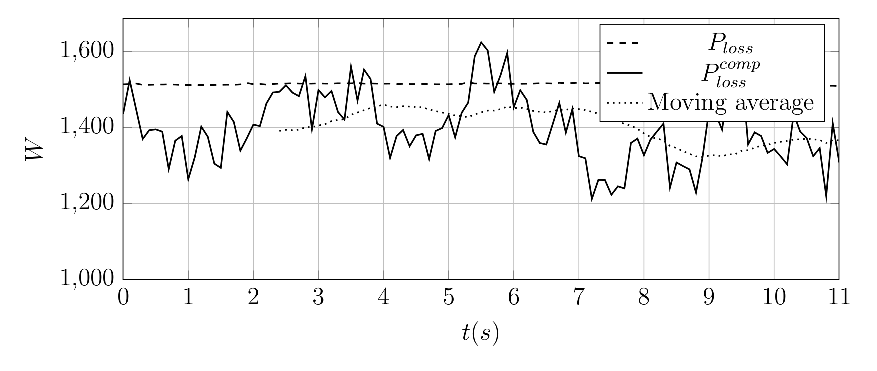
\includegraphics[width=0.95\textwidth]{Unblance_EPS_Pics/UnbalRedComp_JCP-figure6.eps}
%%             %\pgfplotsset{every tick label/.append style={font=\tiny},legend style={at={(1,1)},anchor=north east}}
%%             \pgfplotsset{every tick label/.append style={font=\normalsize}}
%%             \begin{tikzpicture}
%%             \begin{axis}[
%%             width=\textwidth,
%%             height=6cm,
%%             xlabel = {${t(s)}$},
%%             ylabel = {${W}$},
%%             grid=major,
%%             xmin=0,
%%             xmax=20,
%%             ymin=1000,
%%             ]
%%             \addplot[dashed,thick] table {netw_plot_nocont/P_loss.dat};
%%             \addplot[thick] table {netw_plot/P_loss.dat};
%%             \addplot[dotted,thick] table {netw_plot/P_loss_mean.dat};
%%             \legend{$P_{loss}$,$P^{comp}_{loss}$,Moving average}
%%             \end{axis}
%%             \end{tikzpicture}
%            \caption{Compensation control's loss reduction during zero energy balance operation on the modeled network, where $P_{loss}$ indicates the effective power losses and $P^{comp}_{loss}$ effective power losses during control of the network. As result the network losses reduced by mean $6.5\%$.}
%            \label{fig:compare_power}
%            \end{figure*}
%            The results show that despite of the negative cross effects of the intermediate voltage controller and the unbalance reduction controller it was possible to find the trade-off between the control goals of the different controllers (maintain zero energy balance for the inverter and decrease the unbalance on the network). The estimated loss reduction in the experimental setup is 6.5\%.
%            \begin{figure*}[ht]
%            \centering
%            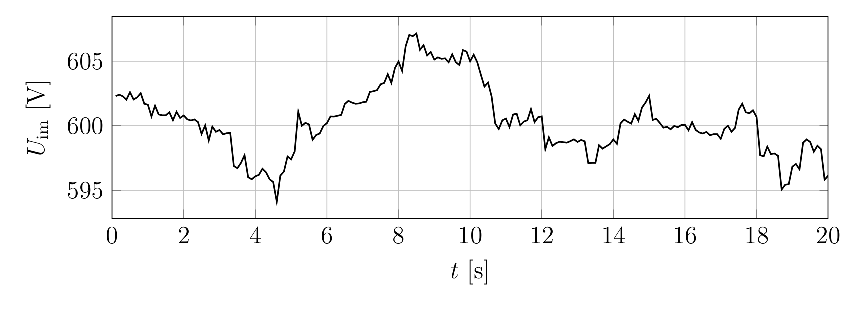
\includegraphics[width=0.95\textwidth]{Unblance_EPS_Pics/UnbalRedComp_JCP-figure7.eps}
%%                  %\pgfplotsset{every tick label/.append style={font=\tiny},legend style={at={(1,1)},anchor=north east}}
%%                 \pgfplotsset{every tick label/.append style={font=\normalsize}}
%%                 \begin{tikzpicture}
%%                 \begin{axis}[
%%                     width=\textwidth,
%%                     height=5cm,
%%                     xlabel = {$t$~[s]},
%%                     ylabel = {$U_{\textnormal{im}}$~[V]},
%%                     grid=major,
%%                     xmin=0,
%%                     xmax=20,
%%                     %ymin=0,
%%                     ]
%%                     \addplot[thick] table {netw_plot/U_inter.dat};
%%                     %\legend{\scriptsize$U_{intermediate}$}
%%                     \end{axis}
%%                  \end{tikzpicture}
%                 \caption{Intermediate puffer capacitance's voltage within boundaries ($600\pm10$\,V), during zero energy balance operation mode of the voltage unbalance compensation controller. $U_{\textnormal{im}}$ indicates intermediate the capacitance's voltage.}
%                 \label{fig:u_inter}
%                \end{figure*}
%
%        \paragraph[CO2 footprint]{CO$_2$ footprint}
%
%            The fact that this controller enables the reactive power reduction has a favourable consequence, i.e. the power loss or equivalently CO$_2$ emission and the carbon footprint can also be decreased. The estimated environmental effects of voltage asymmetry compensation can be calculated. Let us assume 3000\,kWh for the yearly electric energy consumption an average household and $9.173\%$ for the loss of the distribution network \cite{MVM2013}. With the controller the losses on the simulated network are reduced by 6.5\%. The calculation follows (\ref{eqn:co_emission})
%
%            \begin{equation}
%                \label{eqn:co_emission}
%                \begin{array}{rcl}
%                 P_{loss}&=&3000\,\textnormal{kWh}\cdot9.173\%\\
%                P^{comp}_{loss}&=&3000\,\textnormal{kWh}\cdot(9.173\cdot0.93)\%\\
%                 \Delta P_{loss}&=&P_{loss}-P^{comp}_{loss}\\
%                 \end{array}
%                \end{equation}
%
%            where $P_{loss}$ is the assumed network loss per household and $P^{comp}_{loss}$ is s the assumed network loss with unbalance compensation control and $\Delta P_{loss}$ is the saved energy. According to (\ref{eqn:co_emission}), unbalance compensation results in an energy savings of 19.26 kWh. Taking into account the proportion of power currently generated by fossil fuels (coal 17.3\,\%, gas 38.3\% \cite{MVM2013}, \cite{gorbe2012reduction}) and the rate of $\textnormal{CO}_2$ emission during electric energy production (1,000\,g/kWh from coal and 430\,g/kWh from gas), it can be concluded that voltage unbalance compensation could reduce $\textnormal{CO}_2$ emissions by 6504.9\,g a year, in an average household. %Note that this result reflect only the proof of concept, due the neglected power losses of the inverter and the artificial load of the network.
%
%
%\subsection{Conclusion}
%
%    The currently used measures of voltage unbalance has been extended in this work with a norm candidate. It is more demanding from the computational point of view but has an interesting feature namely it checks electrical asymmetry, i.e. the norm of a $\pm120$ degree  rotated version of the ideal three-phase phasor is zero in the geometrical sense.\\
%    The defined norm is applied as a cost function in the asymmetry reducing controller structure also presented in the paper. Simulations show that the geometrical based unbalance indicator can serve as a basis of further research. The suggested controller structure enables the residential users owning a grid synchronized domestic power plant to reduce voltage unbalance measurable at the connection point. The fundamental element of the system is a modified three phase inverter that is capable of the asymmetric injection of any current waveforms to the network. The optimization based control algorithm injects the available energy (as current waveform) in such a way, that the voltage unbalance decreases. This optimization problem is usually constrained by the available renewable energy supplied by the power plant.\\
%    The control structure has been tested on a low voltage network model in a dynamical simulation environment consisting of the models of the electrical grid, a domestic power plant,  asymmetrical inverter circuit, and different types of loads. Different simulation experiments has been run for each norm and for both the power constrained and unconstrained case. The preliminary results show that this structure can serve as a residential level voltage quality improvement method for the three phase low voltage network.



%% Explicit MPC
\section{Explicit predictive control for current source buck-type rectifiers.}

First half with MPC goodies!

\subsection{Mathematical Modeling of the CSR}

    The structure of the classical three phase buck-type current source rectifier (CSR) is presented in \ref{EMPC:fig:network}. In continuous current mode, the differential equations corresponding to the CRS’s inductor currents and capacitor voltages are the following:

    \begin{figure}[!ht]
        \centering
        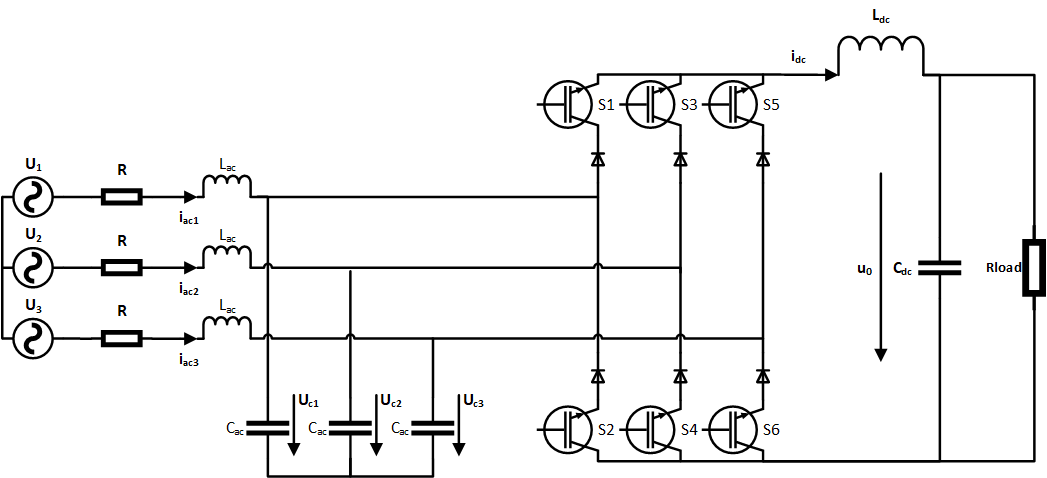
\includegraphics[width=\textwidth]{EMPC_PNG_Pics/circuit.png}
        \caption{Circuit diagram of the three-phase buck-type rectifier with insulated gate bipolar transistors (IGBTs).}
        \label{EMPC:fig:network}
    \end{figure}
        \begin{equation}
        \begin{array}{rcl}
            L_{ac}\dot{i_{ac_p}}&=&u_p-u_{c_p}-Ri_{ac_p}\\
            C_{ac}\dot{u_{c_p}}&=&i_{ac_p}-\delta_pi_{dc}\\
            L_{dc}\dot{i_{dc}}&=&(\sum_{p=1}^{3}\delta_pu_{c_p})-u_0\\
            C_{dc}\dot{u_0}&=&i_{dc}-\frac{u_0}{R_{load}}\\
        \end{array}
        \label{EMPC:equ:abc_eqn}
    \end{equation}

    where $p\in\{1,2,3\}$ is the index of three phases and $\delta_p$ describes the conduction state of the rectifier leg p \ref{EMPC:equ:delta_set}.

    \begin{equation}
        \begin{array}{rcl}
            \delta_p&=&\begin{Bmatrix}
                \textrm{1 if the upper transitor is ON}\\
                \textrm{-1 if the lower transistor is ON}\\
                \textrm{0 if both are ON or OFF}
            \end{Bmatrix}
        \end{array}
        \label{EMPC:equ:delta_set}
    \end{equation}

    Using the components in the stationary frame of the space phasors of the three-phase quantities, from \ref{EMPC:equ:abc_eqn} it results:

    \begin{equation}
        \begin{array}{rcl}
            L_{ac}\dot{i_{ac_\alpha}}&=&u_\alpha-u_{c_\alpha}-Ri_{ac_\alpha}\\
            L_{ac}\dot{i_{ac_\beta}}&=&u_\beta-u_{c_\beta}-Ri_{ac_\beta}\\
            C_{ac}\dot{u_{c_\alpha}}&=&i_{ac_\alpha}-\delta_\alpha i_{dc}\\
            C_{ac}\dot{u_{c_\beta}}&=&i_{ac_\beta}-\delta_\beta i_{dc}\\
            L_{dc}\dot{i_{dc}}&=&1.5(\delta_\alpha u_{c_\alpha}+\delta_\beta u_{c_\beta})-u_0\\
            C_{dc}\dot{u_0}&=&i_{dc}-\frac{u_0}{R_{load}}\\
        \end{array}
        \label{EMPC:equ:abc_alfabeta}
    \end{equation}

    Equation \ref{EMPC:equ:abc_alfabeta} is transformed to the synchronous reference frame rotating with the $u_{c_d}$ capacitor voltage space vector. The resulting mathematical model is thus:

    \begin{equation}
        \begin{array}{rcl}
            L_{ac}\dot{i_{ac_d}}&=&u_d-u_{c_d}-Ri_{ac_d}+\omega L_{ac}i_{ac_q}\\
            L_{ac}\dot{i_{ac_q}}&=&u_d-u_{c_q}-Ri_{ac_q}-\omega L_{ac}i_{ac_d}\\
            C_{ac}\dot{u_{c_d}}&=&i_{ac_d}-\delta_di_{dc}+\omega C_{ac}u_{c_q}\\
            C_{ac}\dot{u_{c_q}}&=&i_{ac_q}-\delta_qi_{dc}-\omega C_{ac}u_{c_d}\\
            L_{dc}\dot{i_{dc}}&=&1.5(\delta_d u_{c_d}+\delta_q u_{c_q})-u_0\\
            C_{dc}\dot{u_0}&=&i_{dc}-\frac{u_0}{R_{load}}\\
        \end{array}
        \label{EMPC:equ:abc_dq}
    \end{equation}

    where $\omega_s$ represents the network voltage vector’s angular velocity.

    \subsection{Model simplification}

    Notice, that the sixth-order ODE model (4) is bilinear in its states and
    inputs because of the product terms (e.g.: $\delta_di_{dc}$). As such, using design methods for linear systems is not straightforward. The high complexity given by the system’s order is another problem to tackle. For designing classic MPC, linear, low-order equation systems are favorable. Hence simplification of the model would bring noteworthy benefits, making the MPC design more straightforward, when a linear system resulted.
    Since the AC and DC side’s time constants differ significantly (as in the AC: $\omega_{ac}=\frac{1}{\sqrt{L_ac C_ac}}\cong5.7\cdot10^3$ [rad/s], and on the DC: $\omega_{dc}=\frac{1}{\sqrt{L_dc C_dc}}\cong2.8\cdot10^2$ [rad/s], see Table X. for reference). Thus, the differential equations can be separated into two sets, and the control of the AC and DC sides can be decoupled as described in \cite{ahmed2014model}. The AC side model results as follows:


    \begin{equation}
        \begin{array}{rcl}
            \begin{bmatrix}
                \dot{i_{ac_d}}\\
                \dot{i_{ac_q}}\\
                \dot{u_{c_d}}\\
                \dot{u_{c_q}}
            \end{bmatrix}&=&
            \begin{bmatrix}
                -\frac{R}{L_{ac}}   &\omega &-\frac{1}{L_{ac}}  &0\\
                -\omega   &-\frac{R}{L_{ac}} &0  &-\frac{1}{L_{ac}}\\
                \frac{1}{C_{ac}}   &0 &0  &\omega\\
                0   &\frac{1}{C_{ac}} &-\omega  &0
            \end{bmatrix}
            \begin{bmatrix}
                i_{ac_d}\\
                i_{ac_q}\\
                u_{c_d}\\
                u_{c_q}
            \end{bmatrix}+
            \begin{bmatrix}
                \frac{u_d}{L_{ac}}\\
                \frac{u_q}{L_{ac}}\\
                -\frac{\delta_di_{dc}}{C_{ac}}\\
                -\frac{\delta_qi_{dc}}{C_{ac}}
            \end{bmatrix}
        \end{array}
        \label{EMPC:equ:mtx_AC}
    \end{equation}

    Looking at the state matrix it can be further stated that there are only weak couplings between the $d$ and $q$ components. This allows to handle them separately, and later to design separate control for each.
    The equation system describing the DC side dynamics is the following:

    \begin{equation}
        \begin{array}{rcl}
            \begin{bmatrix}
                \dot{i_{dc}}\\
                \dot{u_{0}}
            \end{bmatrix}&=&
            \begin{bmatrix}
                0&  -\frac{1}{L_{dc}}\\
                \frac{1}{C_{dc}}&   -\frac{1}{R_{load}C_{dc}}
            \end{bmatrix}
            \begin{bmatrix}
                i_{dc}\\
                u_0
            \end{bmatrix}+
            \begin{bmatrix}
                \frac{1.5}{L_{dc}}(\delta_du_{c_d}+\delta_qu_{c_q})\\
                0
            \end{bmatrix}
        \end{array}
        \label{EMPC:equ:mtx_DC}
    \end{equation}

    It can be noticed that, with the AC and DC model separation, bilinearity disappears, since the binding coefficients are present only in the input $(\boldsymbol{u})$ of the DC state space model. Consequently, all equations are linear and with a considerably lower order, making control design much easier and allowing for the application of linear design methods. For the DC side dynamics, the linear time invariant differential equation system’s matrices can be identified for predictive control design purposes:

    \begin{equation}
        \begin{array}{rcl}
            \boldsymbol{x}&=&\begin{bmatrix}
                i_{dc}\\
                u_0
            \end{bmatrix},\\
            \boldsymbol{u}&=&(\delta_d u_{c_d}+\delta_q u_{c_d}),\\
            \boldsymbol{y}&=&u_0,\\
            \boldsymbol{A}&=&\begin{bmatrix}
                0&  -\frac{1}{L_{dc}}\\
                \frac{1}{C_{dc}}&   -\frac{1}{R_{load}C_{dc}}
            \end{bmatrix},\\
            \boldsymbol{B}&=&\begin{bmatrix}
                i_{dc}\\
                u_0
            \end{bmatrix},\\
            \boldsymbol{C}&=&\begin{bmatrix}0 &1\end{bmatrix}.
        \end{array}
        \label{EMPC:equ:mtx_ctrl}
    \end{equation}

    where \textbf{x}, \textbf{u} and \textbf{y} are the state, input and output vectors of the DC-side system, and \textbf{A}, \textbf{B} and \textbf{C} are the state, input and output matrices.
    The circuit parameters used for the implementation of the control structure based on this model are presented in Table \ref{EMPC:tbl:params}.

    \begin{table}[]
    \center
        \begin{tabular}{|l|l|}
        \hline
        PARAMETER      & VALUE  \\ \hline
        \textbf{R}     & 0.3ohm \\ \hline
        \textbf{Rload} & 10ohm  \\ \hline
        \textbf{Lac}   & 1mH    \\ \hline
        \textbf{Ldc}   & 30mH   \\ \hline
        \textbf{Cac}   & 30uF   \\ \hline
        \textbf{Cdc}   & 400uF  \\ \hline
        \textbf{f}     & 50Hz   \\ \hline
        \textbf{fpwm}  & 20kHz  \\ \hline
        \textbf{Un}    & 400V   \\ \hline
        \end{tabular}
        \caption{The applied parameters in model and controller design}
        \label{EMPC:tbl:params}
    \end{table}

\subsection{Control structure}

    Relying on the possibility of separation of the AC-side and DC-side controllers, the control structure from Fig. \ref{EMPC:fig:ControlStruct}. is proposed.

    \begin{figure}[!ht]
        \centering
        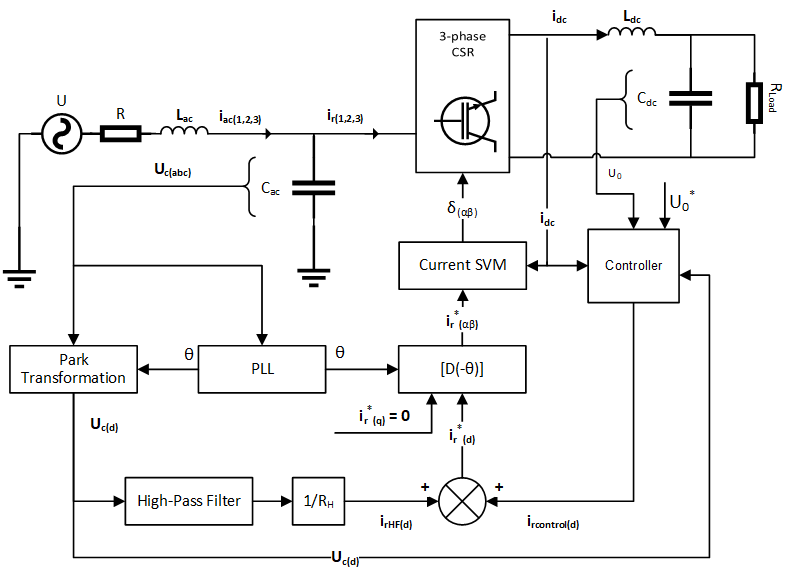
\includegraphics[width=\textwidth]{EMPC_PNG_Pics/ControlStructure.png}
        \caption{Block diagram of the control structure.}
        \label{EMPC:fig:ControlStruct}
    \end{figure}

    The controllers operate in the synchronous frame of the AC filter capacitor voltages $u_{c_{(1,2,3)}}$, and the rectifier input currents $i_{r_{(1,2,3)}}$ are in phase with the capacitor voltages.
    The current reference $i^*_{\alpha\beta}$ supplied to the space vector modulation unit in the stationary frame, is obtained by coordinate transformation $[D(-\Theta)]$ of the current reference \ref{EMPC:equ:sync_ctrl} delivered by the current controllers in the synchronous frame.

    \begin{equation}
        \begin{array}{rcl}
            \begin{Bmatrix}
                i^*_{r_d}=i_{rcontrol_d}+i_{rHF_d}\\
                i^*_{r_q}=0
            \end{Bmatrix}
        \end{array}
        \label{EMPC:equ:sync_ctrl}
    \end{equation}

    In \ref{EMPC:equ:sync_ctrl}, $i_{rcontrol_d}$ represents the output of the DC voltage controller, while $i_{rHF_d}$ represents the damping current, proportional with the high frequency component of the filter capacitor voltage (the fundamental component of the capacitor voltage in the stationary frame becomes a DC component in the synchronous frame). The DC and AC side control units are explained in more detail in the following sections, and the performance of the control structure is evaluated.

\subsection{DC-side explicit model predictive control}

    Model predictive control (MPC) is an efficient and systematic method for solving complex multi-variable constrained optimal control problems \cite{vajda2017limiting}. The MPC control law is based on the “receding horizon formulation”, where the model’s assumed behavior is calculated for a number of N steps, where N stands for the horizon’s length. Only the first step of the computed optimal input is applied in each iteration. The remaining steps of the optimal control input are discarded and a new optimal control problem is solved at the next sample time. Using this approach, the receding horizon policy provides the controller with the desired feedback characteristics, although with high order systems the computational effort is considerably demanding since all the steps should be taken in to account on the specified horizon in every iteration. With Explicit MPC (EMPC), the discrete time constrained optimal control problem is reformulated as multi-parametric linear or quadratic programming. Using this approach, the problem of optimization can be solved offline, making it much more feasible from the perspective of the optimal control task. The optimum control law is a piecewise affine function of the states, and the resulting solution is stored in a pre-calculated lookup table. The parameter space, or the state-space is partitioned into critical regions. The real-time implementation consists in searching for the active critical region, where the measured state variables lie, and in applying the corresponding piecewise affine control law to achieve the desired dynamics.
    In order to introduce the MPC implementation from this paper, let us consider a linear discrete time system \ref{EMPC:equ:DiscreteStateSpace} derived with the discretisation of system \ref{EMPC:equ:mtx_DC} with zero-order hold method, where control inputs are assumed piecewise constant over the simulation sample time $T_s=\frac{1}{f_s}$ :

    \begin{equation}
        \begin{array}{rcl}
            \boldsymbol{x}(t+1)&=&\boldsymbol{A}_d\boldsymbol{x}(t)+\boldsymbol{B}_d\boldsymbol{u}(t)\\
            \boldsymbol{y}(t)&=&\boldsymbol{C}_d\boldsymbol{x}(t)
        \end{array}
        \label{EMPC:equ:DiscreteStateSpace}
    \end{equation}

    where $\textbf{A}_d$, $\textbf{B}_d$, $\textbf{C}_d$ ere the matrices of the discretised system derived from \ref{EMPC:equ:mtx_ctrl}. With system \ref{EMPC:equ:DiscreteStateSpace} appears to be linear time invariant, MPC design can be followed. The following constraints have to be satisfied:

    \begin{equation}
        \begin{array}{r}
            \boldsymbol{y}_{min}\leq\boldsymbol{y}(t)\leq\boldsymbol{y}_{max},\\
            \boldsymbol{u}_{min}\leq\boldsymbol{u}(t)\leq\boldsymbol{u}_{max}
        \end{array}
        \label{EMPC:equ:contraint_desc}
    \end{equation}

    where $t>0$, $\textbf{x}\in \mathbb{R}^n$, $\textbf{u}\in \mathbb{R}^m$, $\textbf{y}\in \mathbb{R}^p$. The MPC solves the following constrained optimization problem \cite{rivera2013predictive}:

    \begin{equation}
        \begin{array}{rcl}
           \displaystyle \min_{U=\{u_t\dots u_t+N_u-1\}}J(\boldsymbol{u},\boldsymbol{x}(t))&=&\sum^{N_y-1}_{k=0}(\boldsymbol{x}^T_{t+N_y|t}\boldsymbol{Q_w}\boldsymbol{x}_{t+N_y|t}+
           \boldsymbol{u}^T_{t+k}\boldsymbol{R_w}\boldsymbol{u}_{t+k})\\
        \end{array}
        \label{EMPC:equ:optim_problem}
    \end{equation}

    subject to:

    \begin{equation}
        \begin{array}{l}
            \boldsymbol{x}_{min}\leq\boldsymbol{x}_{t+k|t}\leq\boldsymbol{x}_{max},\,k=1,\dots,N_c-1\\
            \boldsymbol{u}_{min}\leq\boldsymbol{u}_{t+k|t}\leq\boldsymbol{u}_{max},\,k=1,\dots,N_c-1\\
            \boldsymbol{x}_{t|t}=\boldsymbol{x}(t),\,\boldsymbol{u}_{t|t}=\boldsymbol{u}(t)\\
            \boldsymbol{x}_{t+k+1|t}=\boldsymbol{A}_d\boldsymbol{x}_{t+k|t}+\boldsymbol{B}_d\boldsymbol{u}_{t+k|t}\\
            \boldsymbol{y}_{t+k|t}=\boldsymbol{C}_d\boldsymbol{x}_{t+k|t}\\
            \boldsymbol{u}_{t+k|t}=-K\boldsymbol{x}_{t+k|t},\,k\geq0\\
        \end{array}
        \label{EMPC:equ:optim_problem_constr}
    \end{equation}

    This problem is solved at each time instant $t$, where $\textbf{x}_{t+k\vert t}$ denotes the state vector predicted at time $t+k$, obtained by applying the input sequence $\textbf{u}_{t|t}...\textbf{u}_{t|t+1}$ to model \ref{EMPC:equ:quadratic_regions}, starting from the state $\textbf{x}_{t|t}$. Further, it is assumed that $Q$ and $R$, are symmetric positive semidefinite $(Q_w=Q_w^t\geq0,\_R_w=R_w^t>0)$ and $K$ is a feedback gain. Further, $N_y,N_u,N_c$ are the output, input and constraint horizons, respectively.
    Using the model for predicting the future behavior of the system and with some appropriate substitution and variable manipulation, the problem \ref{EMPC:equ:optim_problem},\ref{EMPC:equ:optim_problem_constr} can be transformed to the standard multi parametric quadratic programming (mp-QP) form, as described in \cite{rivera2013predictive}:

    \begin{equation}
        \begin{array}{rcl}
            V_z&=&min\frac{1}{2}z^tHz
        \end{array}
        \label{EMPC:equ:quadratic_program}
    \end{equation}

    subject to:

    \begin{equation}
        \begin{array}{rcl}
            Gz&\leq&W+S\boldsymbol{x}(t)
        \end{array}
        \label{EMPC:equ:quadratic_inequality}
    \end{equation}

    where the matrices $H$, $G$, $W$, $S$ result directly from the coordinate transformations and variable manipulations. The solution of the mp-QP problem for each critical region has the form:

    \begin{equation}
        \begin{array}{rcl}
            \boldsymbol{u}^*&=&f_i\boldsymbol{x}+g_i
        \end{array}
        \label{EMPC:equ:quadratic_regions}
    \end{equation}

    and the critical region is described by:

    \begin{equation}
        \begin{array}{rcl}
            \mathcal{C}_{reg_i}&=&\{\boldsymbol{x}\in R^n|H_i\boldsymbol{x}\leq K_i\}
        \end{array}
        \label{EMPC:equ:quadratic_critical}
    \end{equation}

    Thus, the explicit MPC controller is completely characterized by the set of parameters:

    \begin{equation}
        \begin{array}{l}
            \{f_i,g_i,H_i,K_i\}^{i=1\dots N}
        \end{array}
        \label{EMPC:equ:quadratic_set}
    \end{equation}

    In case of the discrete time system resulting from \ref{EMPC:equ:mtx_ctrl}, for sampling time equal with the switching period $T_s=5\cdot10^{-5}$  s, the problem defined to be solved by MPC is the minimization of the quadratic cost function \ref{EMPC:equ:DiscreteStateSpace} for:

    \begin{equation}
        \begin{array}{l}
            \boldsymbol{R}_w=\begin{bmatrix}
                1& 0\\
                0& 1\\
            \end{bmatrix},
            \boldsymbol{Q}_w=\begin{bmatrix}
                10^{-6}& 0\\
                0& 10^{-6}\\
            \end{bmatrix},
            N_y=N_u=N_c=2
        \end{array}
        \label{EMPC:equ:quadratic_mtx_set}
    \end{equation}

    Since $N_y,N_u,N_c$ take the same value, they will be substituted by $N$.
    The constraints defined based on the rated power of the CSR $P_n=2500$ W, are:

    \begin{equation}
        \begin{array}{rcl}
            0\leq&i_{dc}&\leq 50A\\
            0\leq&u_{0}&\leq 500V
        \end{array}
        \label{EMPC:equ:numeric_constraints}
    \end{equation}

    The state space partition resulting from this problem has 13 critical regions, which can be observed in Fig. \ref{EMPC:fig:regions}.

    \begin{figure}[!ht]
        \centering
        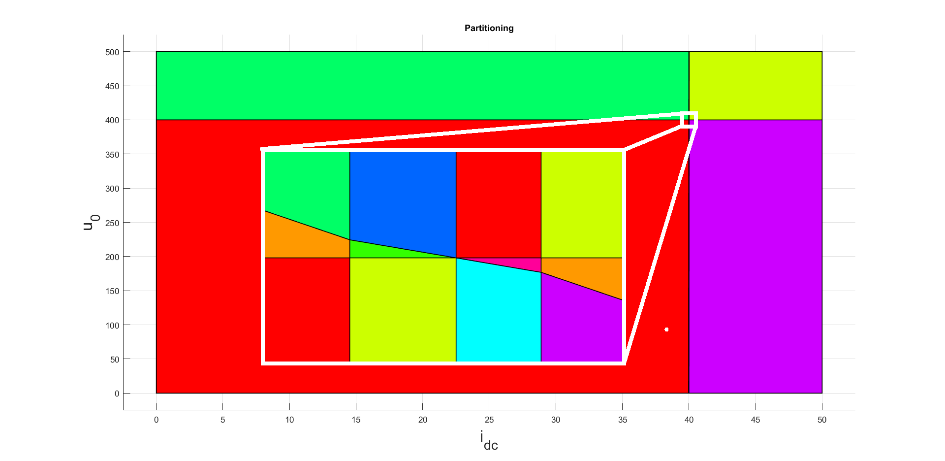
\includegraphics[width=\textwidth]{EMPC_PNG_Pics/Regions.png}
        \caption{State space partitioning.}
        \label{EMPC:fig:regions}
    \end{figure}

    From the basis of the discredited model \ref{EMPC:equ:DiscreteStateSpace}, the given constraints, and horizon \ref{EMPC:equ:numeric_constraints} the cost function \ref{EMPC:equ:optim_problem} is established via the MPT toolbox [30] and used in the generated controller for the EMPC design [29], [31]. The controller is created as a compliable S-function in the Matlab/Simulink environment and its place in the control structure can be observed in Fig. \ref{EMPC:fig:MPCStructure}. as the EMPC controller.
    The output of the MPC controller is the control variable obtained via solving \ref{EMPC:equ:optim_problem_constr} and
    $u_{MPC}=(\delta_du_{c_d}+\delta_qu_{c_q})$, from which the current reference can be calculated using \ref{EMPC:equ:numeric_constraints}. The quadrature component $u_{c_q}$ is zero in the synchronous frame of the filter capacitor voltage.


    \begin{equation}
        \begin{array}{rcl}
            i_{rMPC_{d}}&=&\frac{u_{MPC}}{u_{c_d}}\cdot i_{dc}
        \end{array}
        \label{EMPC:equ:direct_controlval}
    \end{equation}

    \begin{figure}[!ht]
        \centering
        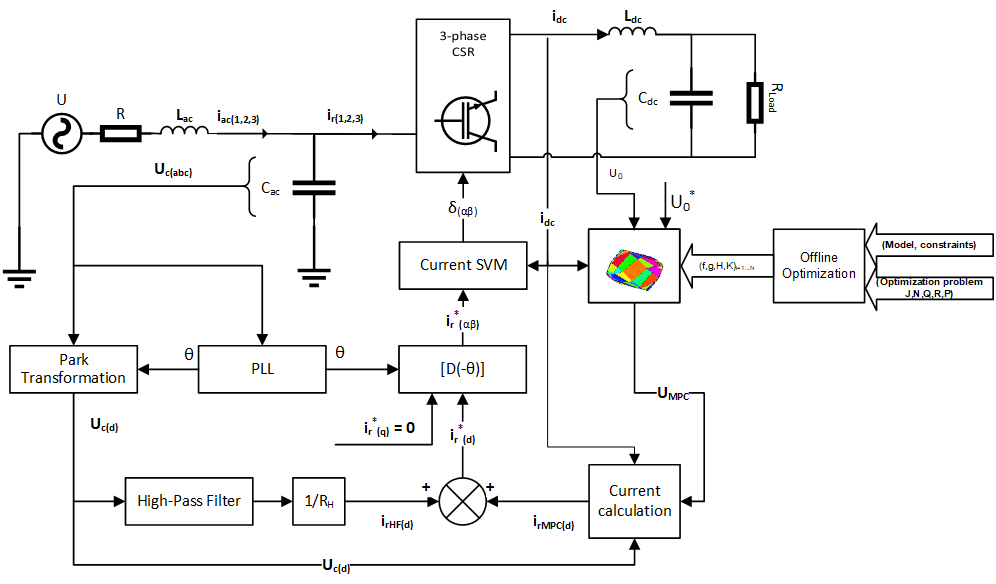
\includegraphics[width=\textwidth]{EMPC_PNG_Pics/MPCStructure.png}
        \caption{The control structure of the CSR, with MPC controller on the DC side.}
        \label{EMPC:fig:MPCStructure}
    \end{figure}

\subsection{Active AC-side damping}

    The CSR requires a voltage supply on the AC side. Taking into consideration the inductive character of the mains, the presence of a three-phase capacitor tank at the input of the CSR is a must. The most convenient is to use three-phase LC filtering with inductors on the lines and star connected capacitors resembling those in Fig. \ref{EMPC:fig:network}, although the resonance phenomena between these components can still cause difficult problems. The simplest way to dampen the resonance on the AC side LC filter is to add a damping resistor across the capacitor \cite{regaya2014new}. Because these resistors result in high losses, active damping methods have been proposed, which emulate damping resistors by control. This makes the CSR bridge produce an additional high frequency current, equivalent to the presence of virtual damping resistors connected in parallel with the AC capacitors. The resonance of the AC side LC filter produces harmonics in the capacitor voltage with frequency close to $\omega_{ac}=\frac{1}{\sqrt{L_{ac}C_{ac}}}$, which appears as $\omega_{ac}-\omega$ component in $u_{c_d}$, where $\omega=2\pi f$. The fundamental component of the capacitor voltage represents a DC component in the synchronous reference frame. Therefore, a high-pass filter (HPF) is applied to filter out this DC component, with the transfer function:

    \begin{equation}
        \begin{array}{rcl}
            HPF(s)&=&\frac{s}{s+0.1\cdot(\omega_{ac}-\omega}
        \end{array}
        \label{EMPC:equ:AC_HPF}
    \end{equation}

    A virtual damping resistance $R_H$ has been defined for calculation of the damping current component $i_{HPF}$ from the HPF component of the capacitor voltage.

\subsection{Space vector modulation strategy}

    The chosen modulation strategy is developed in the $"\alpha\beta"$ stationary reference frame. The structure requires simultaneous conduction of the upper and lower transistors of the bridge, since the current of the $L_{dc}$  choke must not be interrupted. Additionally, the switching devices are considered as ideal.

    \begin{figure}[!ht]
        \centering
        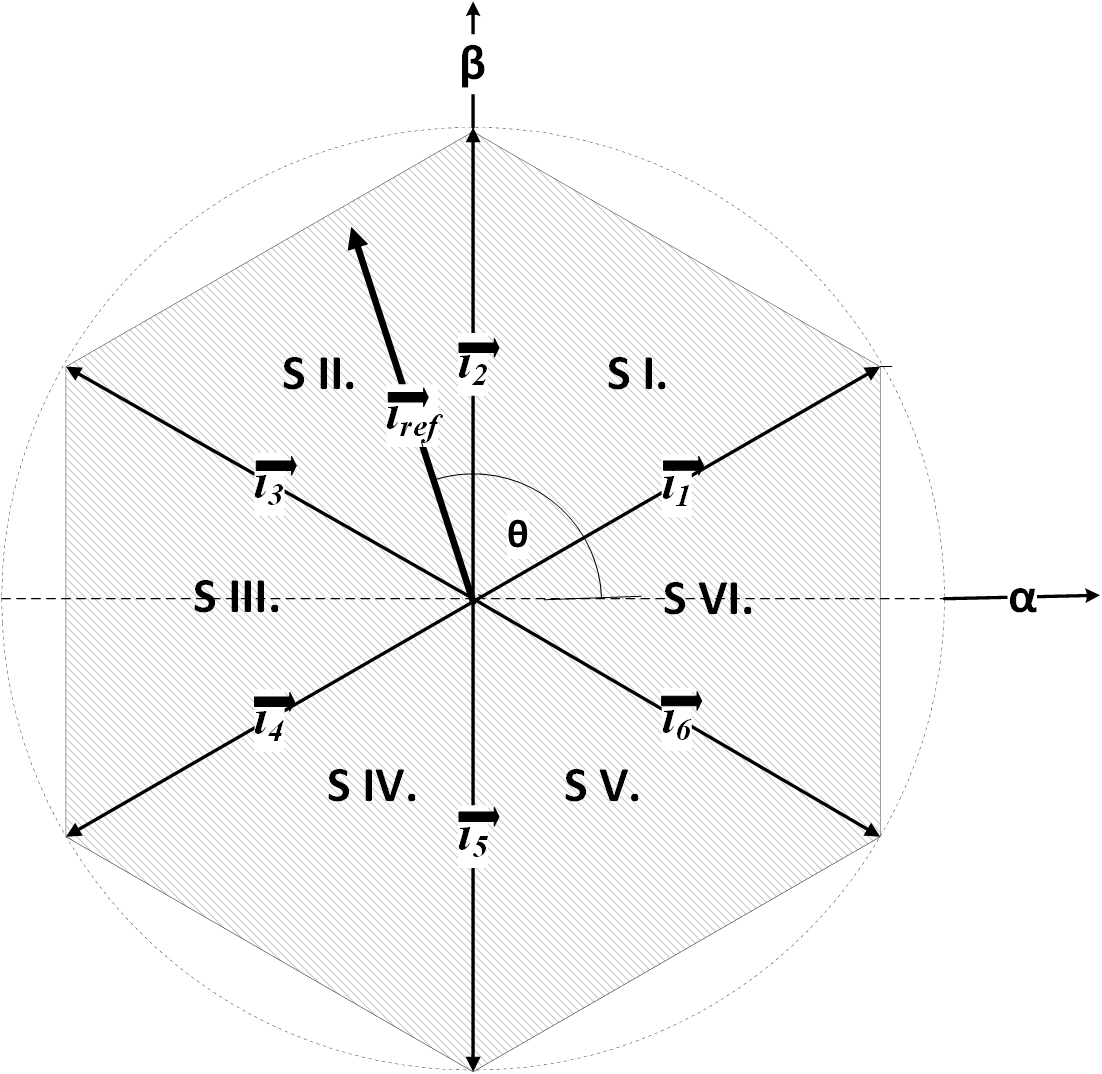
\includegraphics[width=\textwidth]{EMPC_PNG_Pics/VectorPhasor.png}
        \caption{The fundamental input current vectors corresponding to the active switching states of the CSR.}
        \label{EMPC:fig:VectorPhasor}
    \end{figure}

    According to this, one of the upper and one of the lower switches must be closed at all times. This allows nine states, six of which are active. There are three "zero" vectors, corresponding to the switching states, when both devices of one of the bridge legs are in conduction. These current vectors are shown in Table \ref{EMPC:tbl:fundamental_vect}.


% Please add the following required packages to your document preamble:
% \usepackage{multirow}
% \usepackage[table,xcdraw]{xcolor}
% If you use beamer only pass "xcolor=table" option, i.e. \documentclass[xcolor=table]{beamer}

\begin{table}[]

    \begin{tabular}{|l|l|l|l|l|l|l|l|l|l|l|}
    \hline
    \rowcolor[HTML]{EFEFEF}
    \multicolumn{1}{|c|}{\cellcolor[HTML]{EFEFEF}}                                & \multicolumn{6}{c|}{\cellcolor[HTML]{EFEFEF}\textbf{Switching State}}       & \multicolumn{3}{l|}{\cellcolor[HTML]{EFEFEF}\textbf{Phase currents}} & \multicolumn{1}{c|}{\cellcolor[HTML]{EFEFEF}}                                                 \\ \cline{2-10}
    \rowcolor[HTML]{EFEFEF}
    \multicolumn{1}{|c|}{\multirow{-2}{*}{\cellcolor[HTML]{EFEFEF}\textbf{Name}}} & \textbf{1} & \textbf{2} & \textbf{3} & \textbf{4} & \textbf{5} & \textbf{6} & \textbf{ia}           & \textbf{ib}           & \textbf{ic}          & \multicolumn{1}{c|}{\multirow{-2}{*}{\cellcolor[HTML]{EFEFEF}\textbf{Vector representation}}} \\ \hline
    $\vec{i}_1$                                                                           & 1          & 0          & 0          & 0          & 0          & 1          & $i_{dc}$                   & 0                     & -$i_{dc}$                 & $2i_{dc}e^{j\pi/6}/\sqrt{3}$                                                                                           \\ \hline
    $\vec{i}_2$                                                                            & 0          & 0          & 1          & 0          & 0          & 1          & 0                     & $i_{dc}$                   & -$i_{dc}$                 & $2i_{dc}e^{j\pi/2}/\sqrt{3}$                                                                                           \\ \hline
    $\vec{i}_3$                                                                            & 0          & 1          & 1          & 0          & 0          & 0          & -$i_{dc}$                  & $i_{dc}$                   & 0                    & $2i_{dc}e^{j5\pi/6}/\sqrt{3}$                                                                                          \\ \hline
    $\vec{i}_4$                                                                            & 0          & 1          & 0          & 0          & 1          & 0          & -$i_{dc}$                  & 0                     & $i_{dc}$                  & $2i_{dc}e^{j7\pi/6}/\sqrt{3}$                                                                                          \\ \hline
    $\vec{i}_5$                                                                           & 0          & 0          & 0          & 1          & 1          & 0          & 0                     & -$i_{dc}$                  & $i_{dc}$                  & $2i_{dc}e^{j3\pi/2}/\sqrt{3}$                                                                                           \\ \hline
    $\vec{i}_6$                                                                            & 1          & 0          & 0          & 1          & 0          & 0          & $i_{dc}$                   & -$i_{dc}$                  & 0                    & $2i_{dc}e^{j11\pi/6}/\sqrt{3}$                                                                                           \\ \hline
    $\vec{i}_7$                                                                            & 1          & 1          & 0          & 0          & 0          & 0          & 0                     & 0                     & 0                    & 0                                                                                             \\ \hline
    $\vec{i}_8$                                                                            & 0          & 0          & 1          & 1          & 0          & 0          & 0                     & 0                     & 0                    & 0                                                                                             \\ \hline
    $\vec{i}_9$                                                                            & 0          & 0          & 0          & 0          & 1          & 1          & 0                     & 0                     & 0                    & 0                                                                                             \\ \hline
    \end{tabular}
        \caption{The fundamental input current vectors corresponding to the active switching states of the CSR.}
        \label{EMPC:tbl:fundamental_vect}

\end{table}

    The neighboring space phasors can be formulated as:

    \begin{equation}
        \begin{array}{rcl}
            \vec{i}_n&=&\frac{2}{\sqrt{3}}i_{dc}e^{j(\frac{n\pi}{3}-\frac{\pi}{6})}\\
            \vec{i}_{n+1}&=&\frac{2}{\sqrt{3}}i_{dc}e^{j(\frac{n\pi}{3}+\frac{\pi}{6})}\\
            n&=&1,2,\dots,6
        \end{array}
        \label{EMPC:equ:neighbor}
    \end{equation}

    The reference current vector is sampled with fixed sampling period $T_s$. The sampled value of $\overrightarrow{i_{ref}}$ is synthesized as the time average of two neighbouring space phasors adjacent to the reference current:

    \begin{equation}
        \begin{array}{rcl}
            T_n\vec{i}_n+T_{n+1}\vec{i}_{n+1}&=&T_s\vec{i}_{ref}
        \end{array}
        \label{EMPC:equ:i_ref}
    \end{equation}

    $T_n$ and $T_{n+1}$ represent the individual durations of the switching states corresponding to the neighboring vectors. For example, in case of a current reference vector situated in the first sector, $T_1$, $T_2$ and $T_0$ can be calculated using \ref{EMPC:equ:dwelltime}.

    \begin{equation}
        \begin{array}{rcl}
            T_1&=&T_s\frac{i_{ref_\alpha}}{i_{dc}}\\
            T_2&=&T_s\frac{\sqrt{3}}{2i_{dc}}(i_{ref_\beta}-\frac{i_{ref_\alpha}}{\sqrt{3}})\\
            t_0&=&T_s-T_n-T_{n-1}=T_{7,8,9}
        \end{array}
        \label{EMPC:equ:dwelltime}
    \end{equation}

    \begin{figure}[!ht]
        \centering
        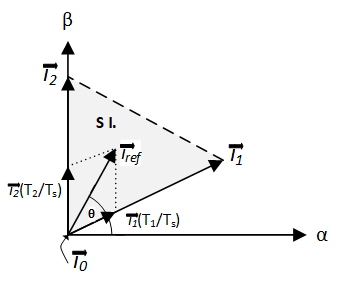
\includegraphics[width=0.8\textwidth]{EMPC_PNG_Pics/OnePhasor.png}
        \caption{Synthesis of $\protect\overrightarrow{i_{ref}}$ by $\protect\overrightarrow{i_{1}}$, $\protect\overrightarrow{i_{2}}$, and $\protect\overrightarrow{i_{0}}$}
        \label{EMPC:fig:OnePhasor}
    \end{figure}

    The complex plane is naturally divided by the fundamental space vectors into six areas, named "sectors".

    \begin{equation}
        \begin{array}{l}
            x\frac{\pi}{6}+\frac{(n-1)\pi}{3}\leq\theta_n\leq\frac{\pi}{6}+\frac{n\pi}{3}\\
            n=1,2,\dots,6
        \end{array}
        \label{EMPC:equ:angle}
    \end{equation}

    The non-zero space vectors are selected based on the phase angle $\theta$ between $\overrightarrow{i_{ref}}$ and the real axis.
    Table \ref{EMPC:tbl:sequence} presents an example of switching pattern in case of a current reference vector situated in Sector I.

    \begin{table}[]
    \centering
        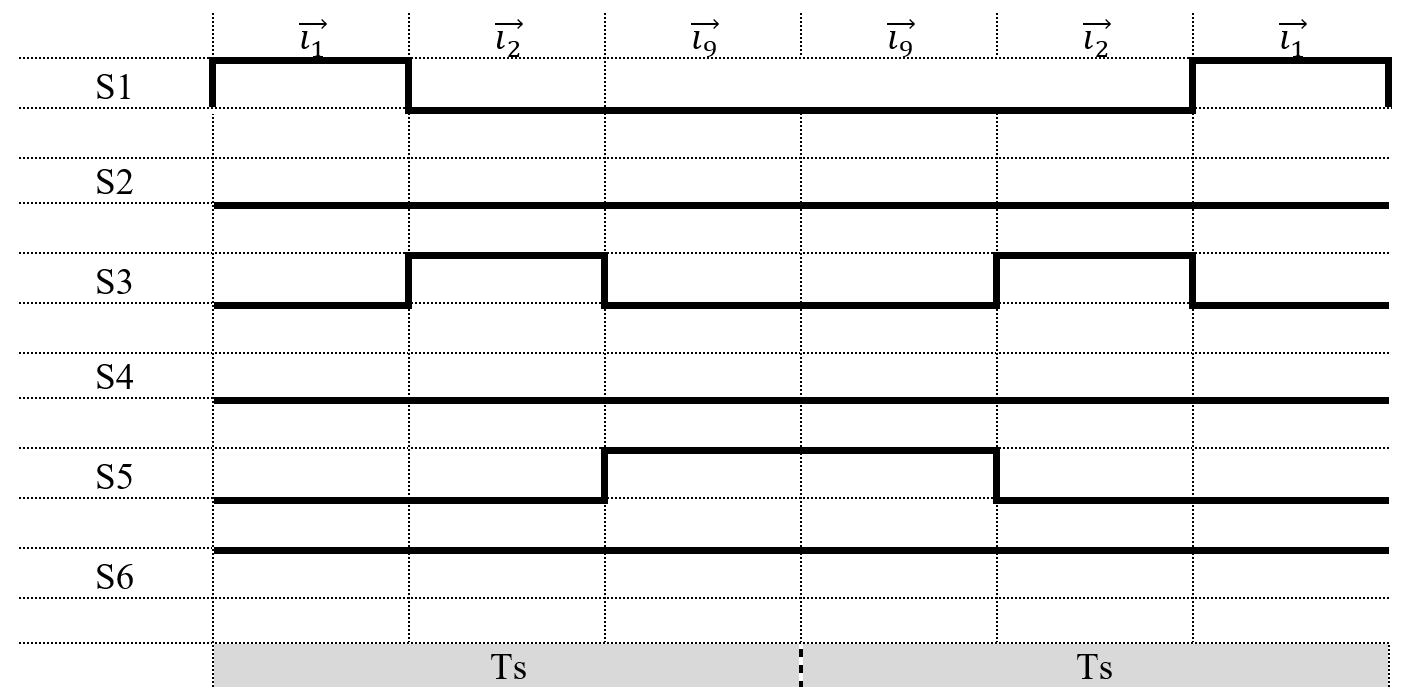
\includegraphics[width=0.8\textwidth]{EMPC_PNG_Pics/Sequence.png}
        \caption{Representation of switching sequences for SECTOR I.}
        \label{EMPC:tbl:sequence}
    \end{table}

    The switching scheme represented in Table \ref{EMPC:tbl:fundamental_vect}. is aimed at reducing the number of commutations in a switching cycle, resulting in the reduction of the switching losses [32].
    Additionally, the constraint (\ref{EMPC:equ:refconstraint}) resulting from the available magnitudes of the current vectors, is applied to the current reference.

    \begin{equation}
        \begin{array}{l}
            0\leq|i_{ref}|\leq\frac{\sqrt{6}i_{dc}}{cos\theta+\sqrt{3}sin\theta}
        \end{array}
        \label{EMPC:equ:refconstraint}
    \end{equation}

\subsection{Performance evaluation}

    From the continuous AC \ref{EMPC:equ:mtx_AC}, and DC \ref{EMPC:equ:mtx_DC} model equations described in Ch.X., the controller is formulated form discretised system \ref{EMPC:equ:DiscreteStateSpace}, and it is described via the cost function and control problem of \ref{EMPC:equ:optim_problem}, and \ref{EMPC:equ:optim_problem_constr} in Ch.X$+$1. The evaluated model and control structure are shown on Fig.4. In the following section said EMPC’s computational requirements are evaluated, and the Matlab/Simulink simulation results are compared to a classic state feedback controller’s dynamic performance.

    \subsubsection{Computational effort}

    The binary search tree generated for the control problem presented in Fig. \ref{EMPC:fig:SearchTree}. The depth of the search tree is 5 and it has a total number of 29 nodes. It is utilized with the MPT toolbox \cite{muthukumar2016adaptive}, \cite{kutasi2010constrained}, and it can be used for the computationally optimal real-time implementation of the proposed algorithm on low-cost hardware.

    \begin{figure}[!ht]
        \centering
        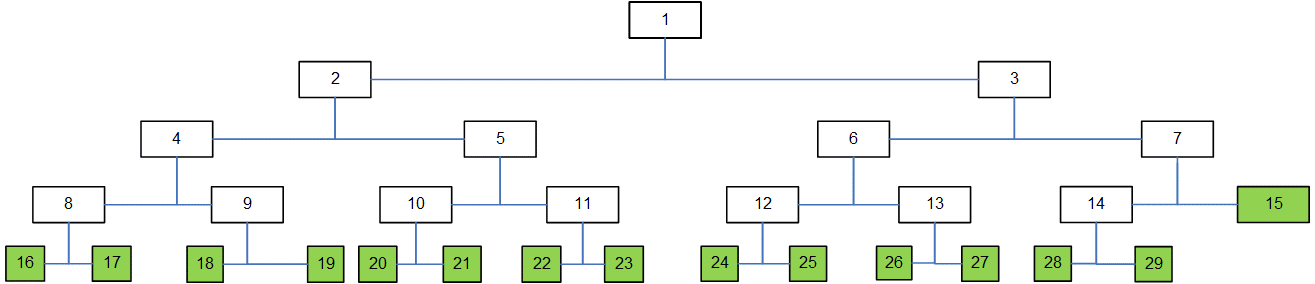
\includegraphics[width=\textwidth]{EMPC_PNG_Pics/SearchTree.png}
        \caption{Binary search tree of the controller for a horizon of N = 4. The leaf nodes are depicted with filled squares. The depth of the tree is 5.}
        \label{EMPC:fig:SearchTree}
    \end{figure}

    The search for an active critical region starts from the first level and represents the evaluation in each adjacent node of an inequality of the form: $x\leq K$. Thus, in this case a maximum number of 4 inequalities have to be evaluated to reach the active critical region. Implementing the presented algorithm is straightforward on a DSP processor, for instance from the dsPIC33 family by Microchip. Using the mac (multiply and accumulate) instruction the inequality is evaluated for each node using 4 instructions, thus in 80ns on a 50MIPS processor (Fig. \ref{EMPC:fig:Memory}). The active critical region can be reached in a maximum of 400ns. Compared to the typical sample rate of 10us in the case of a CSR, the real-time implementation on a DSP processor is possible.

    \begin{figure}[!ht]
        \centering
        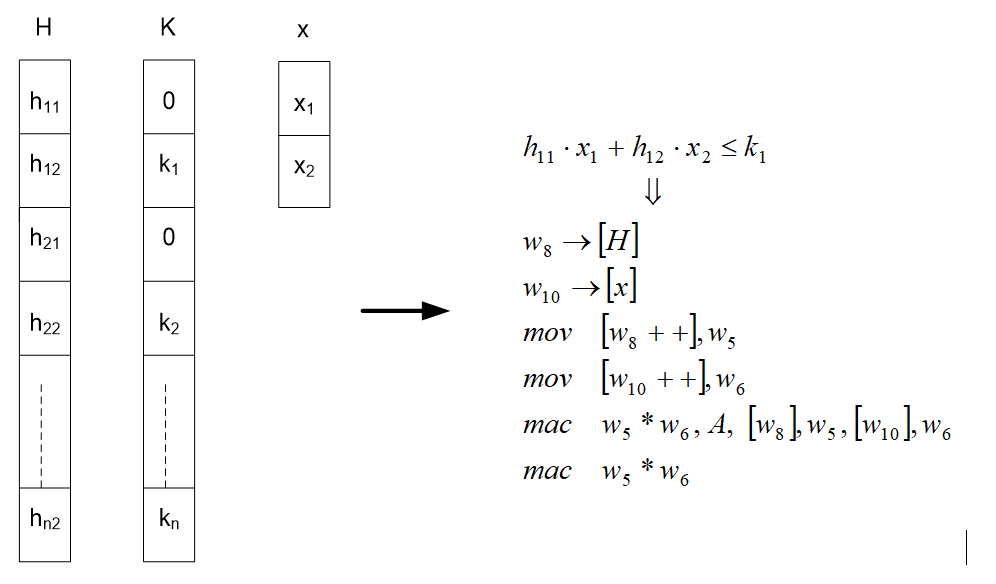
\includegraphics[width=\textwidth]{EMPC_PNG_Pics/Memory.png}
        \caption{Data organization in the data memory of a single core DSP and the evaluation of a 2-dimensional inequality}
        \label{EMPC:fig:Memory}
    \end{figure}

    \subsubsection{Horizon performance}

    With the cost function (\ref{EMPC:equ:optim_problem}) employed using (\ref{EMPC:equ:quadratic_mtx_set}), changing the length of the horizon ($N$) affects the system's complexity illustrated by the partition in the state space shown in Fig. \ref{EMPC:fig:regions}., and Fig. \ref{EMPC:fig:MultiHorizon} presents the step response of the controlled system for different lengths of the horizon. It shows, that the response is not affected by the increase of the horizon above $N=2$, supporting the choice of this value for Matlab Simulink implementation.

    \begin{figure}[!ht]
        \centering
        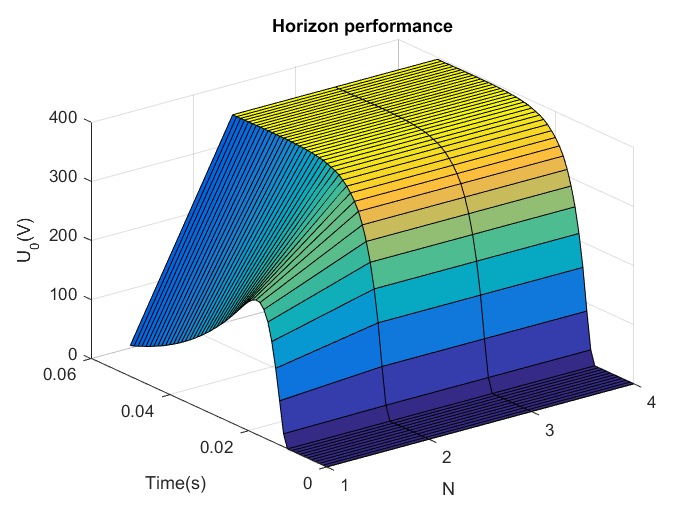
\includegraphics[width=\textwidth]{EMPC_PNG_Pics/MultiHorizon.png}
        \caption{Step response of the system as a function of the horizon length (N).}
        \label{EMPC:fig:MultiHorizon}
    \end{figure}

    \subsubsection{Simulation results}

    The simulation results are produced with Matlab/Simulik. The discrete model's (\ref{EMPC:equ:DiscreteStateSpace}) simulation frequency was 1 MHz, with the model parameters represented in Table \ref{EMPC:tbl:params}., and with the control structure shown on Fig. \ref{EMPC:fig:ControlStruct}. The EMPC performance is shown below:

    \begin{figure}[!ht]
        \centering
        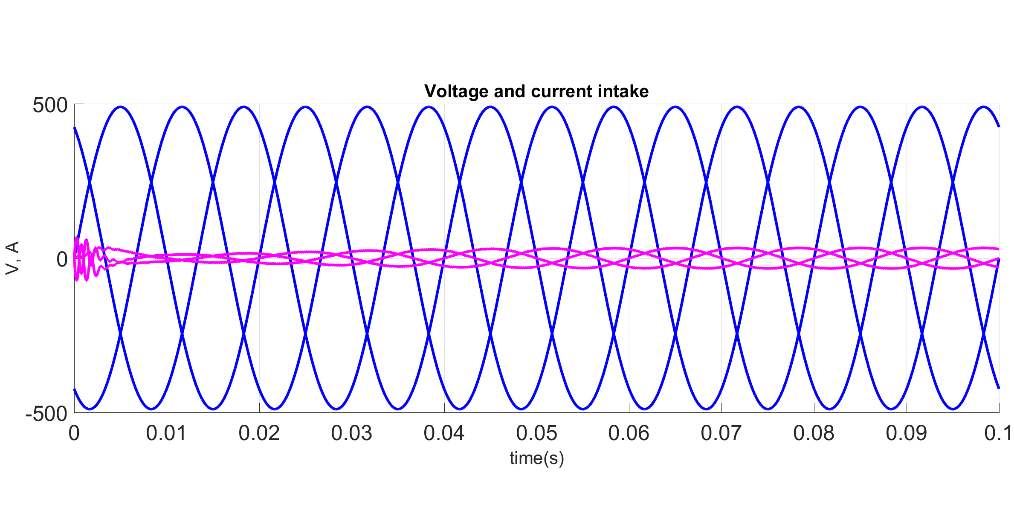
\includegraphics[width=\textwidth]{EMPC_PNG_Pics/Result_3fEMPC.png}
        \caption{Three-phase voltage and current intake of the CSR with EMPC}
        \label{EMPC:fig:Result_3fEMPC}
    \end{figure}

    \begin{figure}[!ht]
        \centering
        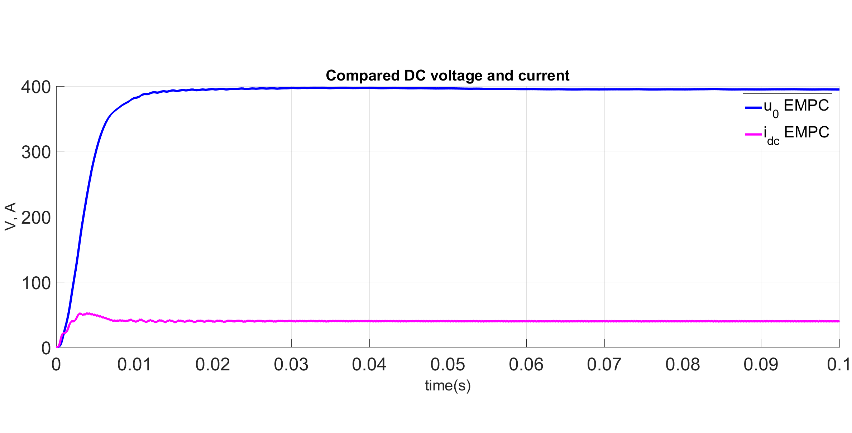
\includegraphics[width=\textwidth]{EMPC_PNG_Pics/Result_PerformanceEMPC.png}
        \caption{Resulting current and voltage trajectories of the CSR with (EMPC).}
        \label{EMPC:fig:Result_PerformanceEMPC}
    \end{figure}

    More details about the Matlab simulation are presented in \cite{neukirchner2019linkedmodel}.

    \subsubsection{Comparison with a state feedback control}

    On the DC side, not only the output voltage $u_0$ but also the inductor current $i_{dc}$ needs to be controlled. Described in [28], a state feedback control with optimal parameters can be used as a reference based on the model properties listed in Table \ref{EMPC:tbl:params}, with output voltage $u_0$ and DC bus current $i_{dc}$ chosen as the state variables. Since $u_0$ is a DC quantity in steady state, an integrator signal is introduced to diminish the steady-state error. The structure of the controller is represented in Fig. \ref{EMPC:fig:SFeedbackDC}.

    \begin{figure}[!ht]
        \centering
        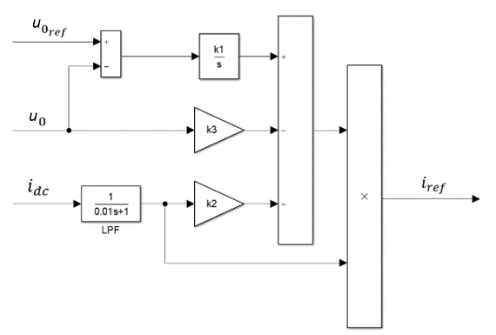
\includegraphics[width=\textwidth]{EMPC_PNG_Pics/SFeedbackDC.png}
        \caption{Simple DC side state feedback control structure.}
        \label{EMPC:fig:SFeedbackDC}
    \end{figure}

    The tuning constants applied and calculated according to \cite{godlewska2015predictive} are:

    \begin{equation}
        \begin{array}{l}
            k1=\frac{\omega^3_n}{1.5U_n\omega^2_{dc}},\,k2=\frac{1.9\omega_n L_{dc}}{1.5U_n},\,k3=\frac{2.2\omega^2_n}{1.5U_n(\omega^2_{dc}-1)},\\
            where,\\
            \omega_n=1.1,\,\omega_{ac}=\frac{1}{\sqrt{L_{ac}C_{ac}}},\,\omega_{dc}=\frac{1}{\sqrt{L_{dc}C_{dc}}}
        \end{array}
        \label{EMPC:equ:tuning}
    \end{equation}

    The state feedback controllers block on the diagram is taking the controller's place, shown on Fig. \ref{EMPC:fig:ControlStruct}. The independent outputs are the high pass filter's output  $i_{rHPF(d)}$ and the controller's output $i_{rcontrol(d)}$. The sum of the independent current values is converted to Clarke frame to be able to govern the switching states of the IGBT's. This can be done because $i_{rHF(d)}$ has only high frequency components and $i_{rcontrol(d)}$ has low frequency components due to the differences in LC time constants, as discussed in the second section. Then the control signal governing the switches is applied in the same manner, described at the start of Section 3.
    The state feedback control's performance in comparison with the EMPC is shown in Fig. \ref{EMPC:fig:Result_EMPCfinal}.

    \begin{figure}[!ht]
        \centering
        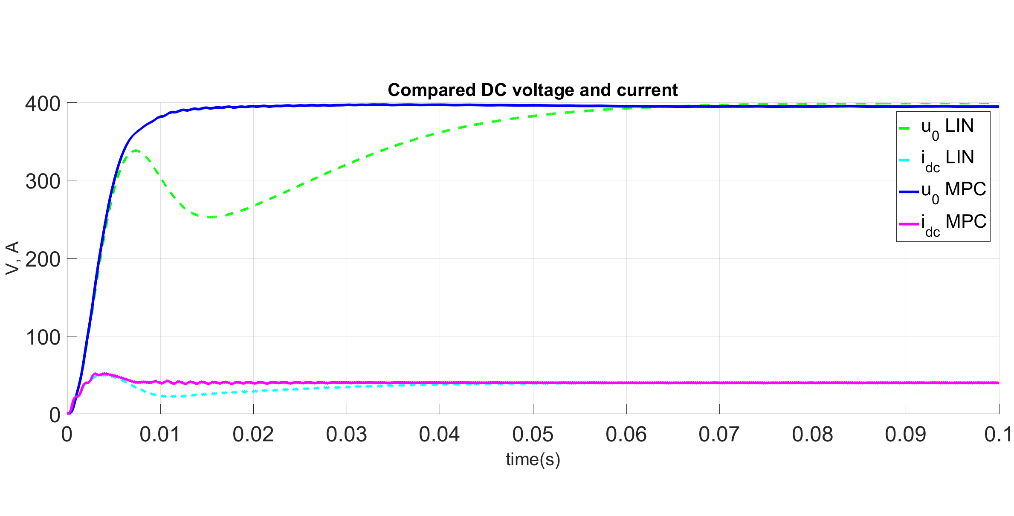
\includegraphics[width=\textwidth]{EMPC_PNG_Pics/Result_EMPCfinal.png}
        \caption{Resulting current and voltage trajectories of the CSR with explicit model predictive control (MPC) compared state feedback control (LIN).}
        \label{EMPC:fig:Result_EMPCfinal}
    \end{figure}

\subsection{Conclusion}

    The constrained, model-based optimal control of a current source rectifier has been presented in this paper. The dynamic model of a three-phase current source rectifier has been developed in Park frame. The proposed model has been examined from the design and implementation points of view with the purpose of explicit model-based predictive control. It proved to be the case that the regular set of differential equations of the CSR appears to be too complex, and contains non-linearity for such a design approach. To address this issue the usage of separated AC and DC equation sets was suggested to avoid linearization and complexity reduction. This solution eliminates bilinearity and enables the application of linear control design techniques. Current-based SVPWM of the three-phase converter has been used with an emphasis on the reduction of switching losses. Throughout the article the explicit model predictive control method is described and the method's effectiveness compared to conventional state feedback control is show. The implementation and simulation experiments have been performed in Matlab/Simulink environment. Moreover, the proper implementation of the system in a modern DSP chip will result in real-time operation. 

%% Summary
\chapter{Thesis and Summary}

\section{Summary}

The topic of this PhD. dissertation is optimal current control. The aim of the research was to apply and simulate high frequency controllers with optimization purpose of cost functions with the presence of constraints and circumstances, on controlled switch based power electronic devices.\\
In chapter \oldref{VUB:sec:Main}, a current controlled inverter structure was presented, connected to a small, domestic grid, representing the connection of a household with possible renewable (or other) generators, to balance consumption. The examined grid, the phenomena of voltage unbalance was assumed to be present, as the main problem, of which this device was ought to not only handle, but mitigate within the limit of its physical capabilities. For this reason, first an indicator was established, based on a proposed geometrical operation, as a voltage unbalance norm candidate (section \oldref{VUB:sec:Geom}). This norm was calculated from the symmetrical difference between the convex hull of voltage phasor vectors, always present on a three phase network. The idea was, that any deviation from the ideal phasor, (which first vector assumed in phase with the ideal one) introduces sub-optimal behavior, or fault of appliances connected. This way the already present indicators of voltage unbalance was examined (section \oldref{VUB:sec:AdditionalContent}). Afterwards found that not only, they vary in result, but ignore phase differences, or the zero-sequence component (based on the Fortescue method), or its ponderous to serve as a cost function need to be minimize. The proposed geometrical norm however considers all of the above, with the addition that since it calculates area, instead of vector length differences, the result is a square-like function, serves as an excellent candidate. The downside is the yet unresolved computational overload, that is method introduces.\\
In the next phase, the network's unbalance was attempted to be mitigated by designing a power electronic converter for a household, which utilizes an external power source (a photo voltaic source in this case) for counter balance (section \oldref{VUB:sec:Compensation}). This way some obstacles needed to be dealt with, first and foremost, the highly stochastic nature of the network. It was assumed, that the device has no external information, rather than the voltage, measured at the network connection point. This way a non-model based asynchronous parallel pattern search (APPS) controller was designed and applied based on the said geometrical norm, which decreases the cost regardless of unknown circumstances. Furthermore, the device needed various subunits, to efficiently handle the power flow in all three phases, namely power-point-tracking, intermediate voltage control, and per-phase current injection was required. The results were tested in Matlab/Simulink environment with simulating the actual device via Simscape, and the unbalanced network, also with experimental measurements. The result was, that the controller could reduce the network's voltage unbalance, based on the network's robustness (how large is the impedance, which created the unbalance), how much control reserve is present as energy source, and physical boundaries (the device can not supply infinite current). Based on this the household's normal operation can withheld even in with unbalanced loads.\\
Lastly in chapter \oldref{EMPC:sec:main} in-depth modeling and predictive control task has been performed, on one power electric component, namely on a buck-type rectifier. This rectifier uses current source operation to supply the load it is connected to. The main goal was to create on the Kirchhoff's law based differential equations a model based predictive controller, suited to reach the reference point with the best dynamics. It was also taken in mind, that an implicit MPC would not be up to the task, sice every control rule was to be re-calculated from scratch, implying a very expensive CPU. This gap could be bridged by reaching out for the explicit MPC method, by partitioning the state space, on a pre-defined rule set. This way the control demand could be reduced significantly, however, this is not suited for high rank systems. As such the system's bi-linearity was eliminated by applying on the premise that two dynamics which have highly different fundamental frequencies can operate in superposition. This way the problem was simplified, and explicit MPC could be implemented in DC-side, whilst active damping at the AC-side. The method's efficiency was tested in Matlab/Simulink environment against a conventional state-feedback controller, with good results. Additionally the computational demand was evaluated, with assumed binary search algorithm.\\

\section{New scientific results}

\begin{enumerate}[I.)]

\item\textbf{Thesis}: \emph{Geometrical indicator for voltage unbalance in three phase networks}\\
    \textbf{Related publications:} \cite{neukirchner2015examination}, \cite{Neukirchner2015}.\\
    I extended the currently used measures of voltage unbalance with a new norm candidate. I found out that it is more demanding from the computational point of view, but has a new feature namely it checks electrical asymmetry, i.e. the norm of a $\pm120$ degree rotated version of the ideal three phase phasor is zero in the geometrical sense. I compared my geometrical approach to the standard wide-spread use of voltage unbalance factor (VUF) and found out it carries additional information, whilst retaining it's original purpose.\\
		
\item\textbf{Thesis}: \emph{Voltage unbalance compensation with optimization based control algorithm and asymmetrical inverter structure}\\
    \textbf{Related publications:} \cite{Neukirchner2015}, \cite{neukirchner2016voltage}, \cite{neukirchner2017voltage}.\\
     I found out that the regular current controlling applications would not fit to the purpose for reducing voltage unbalance whilst only relying on the voltage measurement. As such I developed an asymmetrical current source inverter (ACSI) circuit with combined asynchronous parallel pattern search (APPS) control structure, in Matlab/Simulink environment, and I applied the my geometrical norm as a cost function. I showed with validating simulations, that the geometrical based unbalance indicator can serve as a basis of further research. \\
		The fundamental element of the system is a modified three phase inverter that is capable of the asymmetric injection of any current waveforms to the network. The optimization based control algorithm injects the available energy (as current waveform) in such a way, that the voltage unbalance decreases. The structure enables to show that any point the inverter is connected, could restore power quality with a certain degree such unbalance compensation. This optimization problem is usually constrained by the available renewable energy supplied by the power plant. This suggested controller with combined inverter structure enables the residential users owning a grid synchronized domestic power plant to reduce voltage unbalance measurable at any low voltage domestic the connection point. \\
    I also tested the control structure on a real low voltage network model in a dynamical simulation environment consisting of the models of the electrical grid, a domestic power plant, ACSI, and different types of loads. Different simulation experiments has been run for each norm and for both the power constrained and unconstrained case. I showed with the evaluation that this structure can serve as a residential level voltage quality improvement method for the three phase low voltage network.\\
		
		\item\textbf{Thesis}: \emph{Constrained, explicit predictive control for current source buck-type rectifiers}\\
        \textbf{Related publications:} \cite{neukirchner2020constrained}.\\
    I proposed a simplified CSR model, which was derived from the well known CSR structure and was examined from design and implementation points of view with the purpose of explicit model-based predictive control. The regular set of differential equations of the CSR appeared to be too complex for my a design approach, for applying explicit predictive control. \\
		I adressed this issue with the separation AC and DC equation sets was of the CSR to decrease complexity and easy controller design. With this solution I eliminated bi-linearity and enabled the application of linear control design techniques. I used current-based SVPWM the modulation, what has been used with an emphasis on the reduction of switching losses. \\
		For DC side control I implemented explicit model predictive control (EMPC) and I compared this method's effectiveness to conventional state feedback control. I implemented the CSR structure and the proposed controller with EMPC on DC and active damping on the AC side in Matlab/Simulink environment and tested by simulation. Additionally, I tested the proper implementation's computational requirements in a modern DSP chip, which would serve in real-time operation.\\
	
\end{enumerate}

Publications not related to the thesis:  \cite{neukirchner2011modeling}, \cite{neukirchner2014quasi}, \cite{gollei2014measurement}, \cite{neukirchner2016modelling}.


		\section{Applications and future work}
		
		In this section the possible applications shall be described based on my thesis. These are not yet scope of current research activities, but can serve as a potential direction and evolution for these results.
		
		\subsection{Geometrical voltage unbalance norm}
		
		As mentioned the geometrical norm's largest weakness is the computational demand. The required areas, computed from the voltage phasors realized with the corresponding Matlab functions, which are not designed for continuous calculation, especially not for time constants for power electronic devices. This can be resolved, via replacing the calculation of the symmetrical difference (difference between the two polygon's union and intersection) with finite-element method, with scalability, where the segmentation's resolution would be adjustable and based on the corresponding simulation's (or system's) time constant and the simulator machine's calculation capabilities. After this, the calculation method shall be phrased in an traditional equation form, using the toolset of set theory, and linear algebra. This way, the norm's calculation could be further reduced, and could be implemented on a cheaper embedded system.\\
		The geometrical norm's usefulness was already proven compared o the regular $VUF$ method. However the robustness of the method seems implicitly proven, is shall be tested on real conditions, even in extreme (faulty) situations, and with such hard constrains could be defined, where the algorithm outlives its usefulness. This way, instead of just a resulting number, a full formulation of an optimization problem could be utilized, presented in section \ref{BASICCSR:sec:OptimalControl}, with model based predictive capabilities. This can be further enhanced, with recognizing different scenarios, form general inefficiency, to fault prediction, or handling (like graceful degradation).
		
		\subsection{Voltage unbalance reducing inverter structure}
		
		The inverter structure employ a variety of subsystems, which shall work together in harmony. A global optimum shall be defined (with weighting the various factors) based on external circumstances, and the customers needs. This way, the individual Kirchhoff equations based differential equations shall be established, and controller designed.\\
		The APPS method, however fulfills its optimizing responsibilities very well in such an environment, where changes are expected to be highly stochastic, based on network knowledge, a network- and/or device model based optimal control shall be established, where various current and voltage inertias can be taken into account, giving a leverage for prediction.\\
        \hlc[KP]{The setup of the subsidiary network is is using a very basic network setup. The controller needs to be tested on real world low voltage network models with multiple topologies, and circumstances, established by other research groups and companies, to have a good representation of the system's capabilities.}\\
        \hlc[KP]{The total harmonic distortion (THD) was not in the scope of the research, as such, there was no counter measure implemented in the control cycle, to prevent increasing the system's THD. In an experimental setup this needs to be addressed.}\\
        \hlc[KP]{The controller is not handling reactive power well, means the reactive power evolution was not in the scope of the research, as such due to the unpredictable nature of the network, the injected reactive power could be an issue.}\\
        This way the system's physical properties shall be scalable (based on a household's needs and its energy producing and storing capabilities), as in designing a real power electric system for implementation. Next actual implementation shall be proceeded, with prototype realization on a test bench, with a simulated domestic network connection. Further step to test the presence of multiple of such devices on the network, and how they could mitigate unbalance in synchronous or asynchronous operation. \\
        
		
		\subsection{Explicit model predictive control for buck-type rectifier}
		
		From mathematical perspective it is an alternative possibility to take the harder route and take the inherent bilinearity into account. This way, the devices equations should not be partitioned, and a hybrid design can be commenced. This has been performed in the literature, but seldom on three phase systems, for complexity reasons.\\ The topology could be altered, by removing (or greatly decreasing) some of the device's filtering  capabilities, in inductive or capacitive terms (some inductors, like the choke $L_{dc}$ are non-removable), and try to outsource this problems to the controller itself to some degree.\\
		Try the cost function from Euclidean norm to an infinity norm, and also give stricter constrains. The optimum could be power throughput based instead of a specified current. The types of loads can be extended, and merged with the current equation system. This enables to expand the research on electric machinery, where starting/ breaking dynamics can be tested. On the other side, the effects on the supplying network can be taken into consideration, further reducing harmonics, and test conditions in the presence of unbalance.
		Lastly, experimental results shall be performed on a device, further validating its usefulness, and implement the used S-function from Simulink to an embedded system.
 %--> List of thesis and own publications moved here <=====

%% Nomenclature
%\chapter*{List of notations}



%$\boldsymbol{\Temp{air}{2}}$


%% Abbreviations
\begin{longtable}{r l}
  % after \\: \hline or \cline{col1-col2} \cline{col3-col4} ...
  VSR:      & Voltage source rectifier \\
  CSR:      & Current source rectifier \\
  MPC:      & Model predictive coltrol\\
  MPT:      & Model predictive control toolbox\\
  EMPC:     & Explicit model predictive control\\
  HPF:      & High pass filter\\
  SVPWM     & Space vector pulse width modulated\\
  SFC:      & State feedback control\\
  MDV:      & ?\\
  VUF:      & Voltage unblance factor (i.e. TDV)\\
	CVUF:			& Complex voltage unbalance factor\\
  THD:      & Total harmonic distortion\\
  IGBT:     & Insulated gate bipolar transistor\\
  MPPT:     & Maximum power point tracking\\
	ACSI:			& Asymmetrical current source inverter\\

\end{longtable} 

%% Appendix
%\chapter*{Appendix}
Stuff that is less relevant, or enhance understanding.


%%% Citations
 \newpage
 \pagestyle{plain}
 %\bibliographystyle{plain}
 %% \bibliography{dolgozat_own}
 %\bibliography{dolgozat}

 \boldname{Neukirchner}{L{\'a}szl{\'o}}{L.}   %%%% félkövér kiemeléshez NEM MINDEGY PL. HOGY á VAGY \'a VAN A BIB-BEN !!!!!!!!!!!!
    %\boldname{}{}{}
		\printbibheading
\section*{Publications}
    \begin{refcontext}[labelprefix={P}]
        \printbibliography[keyword=sajat, heading=none, title={asd}]        %% keyword alapján szűr, azaz bele kell tenni a bib-be
    \end{refcontext}

    \section*{Literature}
    %\boldname{}{}{}
    \printbibliography[notkeyword=sajat,resetnumbers=true, heading=none, title={veryasd}] % ha egybe kell a másikkal akkor "heading=none," és nincs title



\end{document}
